\documentclass[12pt,a4paper,final,twoside]{stylevk}
% \usepackage[dvips]{graphicx}
\usepackage{times} 
\usepackage[pdftex]{graphicx}
%
% FDS version  6.7.6
% Evac version 2.6.0
% May 2021
%
\usepackage[T1]{fontenc}
\usepackage[latin1]{inputenc}
\usepackage[english]{babel}
\usepackage{fancyhdr}
\usepackage{upquote}
% upquote works only for verbatim. \char"0D gives correct quote character elsewhere.
%
\usepackage{amsmath}
\usepackage{amssymb}
\usepackage{amsfonts}
\usepackage{array,eqnarray}

\usepackage{hyperref}
%
% \usepackage{color}
% \definecolor{linknavy}{rgb}{0,0,0.50196}
% \definecolor{linkred}{rgb}{1,0,0}
% \definecolor{linkblue}{rgb}{0,0,1}

% \usepackage{caption}
% \usepackage{graphpap}
% \usepackage{rotating}
%%% \usepackage{epsfig,psfrag}
%\usepackage{wrapfig}
%\usepackage{picins}
\usepackage{geometry}
\usepackage{tabularx}
\usepackage{longtable}
\usepackage{lscape}
\usepackage{makeidx} % Create index at end of document
% \usepackage[nottoc,notlof,notlot]{tocbibind} % Put the bibliography and index in the ToC 
\usepackage{float}
\usepackage{lastpage} % Automatic last page number reference.


\IfFileExists{gitrevision.tex}
{\input{gitrevision}}
{\newcommand{\gitrevision}{unknown} }
%
% \usepackage{indentfirst} 
%

% Page layout for the VTT Working Papers (A4 paper)
% top margin 3.0 cm (including top header 1.0 cm)
% bottom margin 3.0 cm + page number (4.0 cm)
% left + right margins 3.0 cm 
%
% Beginning of 2009: VTT Working Papers is in A4 format:
% Main chapters:
% Top margin 5.2 cm, top header 3.5 cm
% Bottom margin 4.8 cm, bottom label 3.5 cm, page number at center
% Header:  Bold Arial 10 pt, 12 pt line height
% Main text: 12 pt Times New Roman, 16 pt line height
% Body text first indent 0.37 cm
%
\setlength{\paperheight}{297mm}
\setlength{\paperwidth}{210mm}
\setlength{\hoffset}{0mm}
\setlength{\voffset}{0mm}

\setlength{\topmargin}{0.0cm}
\setlength{\headheight}{12pt}
\setlength{\headsep}{16pt}
\setlength{\textheight}{227mm}
\setlength{\footskip}{22mm}

\setlength{\textwidth}{150mm}
\setlength{\oddsidemargin}{4.6mm}
\setlength{\evensidemargin}{4.6mm}

\setlength{\parindent}{3.7mm}
\setlength{\parskip}{0pt}
% \setlength{\parskip}{16.0pt plus 3.5pt minus 1.0pt}
\setlength{\baselineskip}{16.0pt plus 3.5pt minus 1.0pt}

% Heading styles for the VTT Working Papers (A4 paper)
% These are (re)defined in stylevk.
% Next are for the new A4 Working Papers 2009
% Heading 1: Arial 18pt bold (large) (Arial ==> textsf Sans Serif)
%            riviväli 20 pt, 130pt tyhjää tilaa ennen otsikkoa
%            otsikon jälkeen 16pt tyhjää
% Heading 2: Arial 14pt bold, 16pt riviväli, 20pt tyhjää ennen, 14pt jälkeen
% Heading 3: Arial 12pt bold, 16pt riviväli, 18pt tyhjää ennen, 14pt jälkeen
% Heading 4: Arial 12pt, 16pt riviväli, 18pt tyhjää ennen, 12pt jälkeen
% Contents: Arial 18pt bold
% Abstract: Arial 18pt bold, riviväli 20pt, 60pt tyhjää ennen, 12pt
%           jälkeen (sis.luetteloon 1. tason otsikkona)
% alkusanojen otsikko: kuten 1. tason otsikko
% sis.luettelon otsikko: kuten 1. tason otsikko, sen jälkeen 24pt tyhjää
% Acknowledgements: Heading 1
% References: Heading 1, text: 10pt, 13pt riviväli, 1.5 cm riippuva
%             sisennys, kappaleen jälkeen 13pt tyhjää
% Captions: Arial 10pt, 13pt riviväli, 12pt tyhjää ennen, 16pt jälkeen


% \renewcommand{\refname}{\textbf{\normalsize REFERENCES}}
% \renewcommand{\figurename}{\normalsize FIGURE}
% \renewcommand{\tablename}{\normalsize TABLE}
% \renewcommand{\refname}{\normalsize REFERENCES}

%% The maximum number of floats on a page
\setcounter{totalnumber}{3}
%% The level of section numbering
\setcounter{secnumdepth}{3}

% How to use the low level font commands:
% Title: Bold, 14 pt, Times Roman
% {\fontsize{14}{17} \selectfont \bf FDS+Evac: Model}

% \pagestyle{plain}
\pagestyle{headings}

\begin{document}

%% % \bibliographystyle{unsrt}


\newcommand{\Timts}[1]{\textnormal{\texttt{\textsl{#1}}}}
\newcommand{\Timtt}[1]{{\tt{#1}}}
%% % \newcommand{\Timtt}[1]{\textnormal{\texttt{#1}}}
%% % \renewcommand\Large{\@setfontsize\Large\@xxxviiipt{23}}
%% %\let`\textasciigrave
%% %\let'\textquotesingle
\newcommand{\QS}{\hbox{\textquotesingle}}

\fancyhead{}
\fancyfoot[C]{\today}
\renewcommand{\headrulewidth}{0.0pt}
\renewcommand{\footrulewidth}{0.0pt}

\begin{titlepage}

  \thispagestyle{fancy}

  \begin{center}

    VTT Technical Research Centre of Finland

    \vspace{20mm}
   \centerline{\includegraphics[clip=true, angle=90, width=150mm
   ]{FIGURES/KansikuvaAtrium}}  
    \vspace{10mm}

    { \normalfont\fontsize{28}{42}\selectfont\bfseries\sffamily
      Fire Dynamics Simulator with Evacuation: FDS+Evac
    }

    \vspace{6mm}

    { \normalfont\fontsize{22}{28}\selectfont\bfseries\sffamily
      Technical Reference and User's Guide }

    { \normalfont\fontsize{14}{18}\selectfont\sffamily
      FDS: \gitrevision \\
      Evac: 2.6.0-draft 
    }

    \vspace{15mm}

    { \normalfont\fontsize{14}{18}\selectfont\sffamily
      Timo Korhonen }

    \vspace{3mm}

    { \normalfont\fontsize{12}{16}\selectfont\sffamily
      VTT}

  \end{center}


\vspace{2cm}
    

\end{titlepage}

\setcounter{page}{4}

\newpage


\chapter*{Preface}
\addcontentsline{toc}{chapter}{Preface}

\noindent This document describes how to simulate human egress using
the evacuation module, FDS+Evac, developed at VTT Technical Research
Centre of Finland, which is fully embedded in Fire Dynamics Simulator
(FDS).  This manual applies to the FDS+Evac version 2.6.0, which is
embedded in the current FDS version (\gitrevision).

% The most up to date version of this manual can be obtained from the FDS+Evac web page at \texttt{http://www.vtt.fi/}\linebreak[4]\texttt{fdsevac/}.

This FDS+Evac Technical Reference and User's Guide does not contain
information on how to operate FDS nor Smokeview, the companion
visualisation programme for FDS.  Their full capabilities are
described in the ``Fire Dynamics Simulator: User's
Guide''~\cite{FDS_UserGuide} and the ''Smokeview, A Tool for
Visualizing Fire Dynamics Simulation Data,  Volume I: User's
Guide''~\cite{SV_UserGuide}.


Certain commercial entities, equipment, or materials may be identified
in this document in order to describe an experimental procedure or
concept adequately.  Such identification is not intended to imply
recommendation or endorsement by VTT Technical Research Centre of
Finland, nor is it intended to imply that the entities, materials, or
equipment are necessarily the best available for the purpose.

\newpage


\chapter*{Disclaimer}
\addcontentsline{toc}{chapter}{Disclaimer}

\noindent VTT Technical Research Centre of Finland makes no warranty,
expressed or implied, to users of FDS+Evac, and accepts no
responsibility for its use.  Users of FDS+Evac assume sole
responsibility for determining the appropriateness of its use in any
particular application; for any conclusions drawn from the results of
its use; and for any actions taken or not taken as a result of
analyses performed using this tool.


Users are warned that FDS+Evac is intended for use only by those
competent in the fields of fire and evacuation simulation, and is
intended only to supplement the informed judgement of the qualified
user.  The software package is a computer model that may or may not
have predictive capability when applied to a specific set of factual
circumstances.  Lack of accurate predictions by the model could lead
to erroneous conclusions with regard to life safety.  All results
should be evaluated by an informed user.


\clearpage

\newpage


\tableofcontents

\newpage

\chapter{Introduction}\label{Sec_Intro}

\noindent This document describes how to simulate human egress using
the Fire Dynamics Simulator (FDS)~\cite{FDS_Manual, FDS_UserGuide,
  FDS_VVGuide1, FDS_VVGuide2}, and in particular, the evacuation
module~\cite{Korhonen05, Korhonen07a, Korhonen07b, Korhonen08a,
  Korhonen08b}.  This combined fire and evacuation simulation
programme is called FDS+Evac in this document.  FDS+Evac allows
simultaneous simulation of fire and evacuation processes.  It can also
be used to simulate only the human egress process without any fire
effects, \emph{e.g.}, a fire drill.


FDS+Evac treats each evacuee as a separate entity, or an 'agent',
which has its own personal properties and escape strategies.  The
movement of the agents is simulated using two-dimensional planes
representing the floors of buildings.  The basic algorithm behind the
egress movement solves an equation of motion for each agent in a
continuous two dimensional space (e.g., a horizontal $xy$-plane) and
time, \emph{i.e.}, FDS+Evac is doing some kind of an artificial
molecular dynamics for the agents.  In this document the two
dimensional spaces are the horizontal $xy$-planes representing the
floors of the considered building and the positive $z$ direction is
taken to point upwards.  The forces acting on the agents consist of
both physical forces, such as contact forces and psychological forces
exerted by the environment and other agents.  The model behind the
movement algorithm is the social force model introduced by Helbing's
group~\cite{Helbing95, Helbing00, Helbing02, Werner03}.  A
modification of the model to describe better the shape of the human
body was introduced by Langston \emph{et al.}~\cite{Langston06}.


This chapter contains some general information on FDS+Evac.  In
Chapter 2, the model documentation is summarised.  Chapter 3 presents
the theoretical model behind the agent movement algorithm and details
on the implementation.  Chapter 4 is dedicated to various verification
tests of the programme and Ch. 5 deals with the sensitivity of the
model to the model parameters.  In Chapter 6, FDS+Evac is validated by
comparing to other evacuation calculation methods and experimental
results.  Chapters 7--11 contain the user's guide, where the inputs of
FDS+Evac are explained.


The user of FDS+Evac should read carefully every chapter of this
manual before starting to use the programme.  The knowledge on the
theoretical method is needed in order to build up the model correctly.
It also helps making the judgement on the applicability and
reliability of the programme in the application in question.  Because
the evacuation calculation is implemented as a module of FDS, the
reader is recommended to read first the User's Guide of FDS and learn
how to do fire simulations.  Even if the user wants to use the
programme without fire, she/he should be acquainted with the FDS in
order to build up the simulation geometry and running the FDS
simulations.


\section{Getting Started}\label{Sec_GetStart}

\noindent The evacuation module is embedded inside the FDS.  Thus, the
running of FDS+Evac evacuation simulation is done similarly as an
ordinary FDS fire simulation.  See the FDS User's
Guide~\cite{FDS_UserGuide} for details.  FDS+Evac results can be
visualised using Smokeview~\cite{SV_UserGuide,SV_TechGuide,SV_VVGuide}
programme.  Also, the computer hardware requirements are similar with
FDS.  The FDS fire calculation can be run parallel by using the MPI
version of FDS, but the evacuation part is always calculated as a
single thread (process).


The evacuation module, FDS+Evac, is embedded in the latest released
version of FDS (FDS 6.5.3), which can be obtained from the URL
\begin{verbatim}
https://pages.nist.gov/fds-smv/
\end{verbatim}
Download the latest version of FDS-Smokeview installation package and
install it.  Check if there exists more recent maintenance releases of
the executables.  The resulting FDS executables are also the
executables of the evacuation calculation module.  The source codes
can also be obtained via the FDS-SMV web pages.  The results of the
FDS+Evac simulations can be visualized using the Smokeview programme
similarly as the fire results.


The home page of FDS+Evac is 
\begin{verbatim}
http://www.vtt.fi/fdsevac/
\end{verbatim}
This page contains the most recent version of this combined Technical
Reference and User's Guide of FDS+Evac and some examples on the use of
FDS+Evac.  This web site is also used to store the validation and
verification test cases including the input files.  This (printed)
manual refers to FDS 6.6.0 + Evac 2.5.2 (GIT FDS6.6.0-986-g47260e6).


\section{Features of Limited Functionality}\label{Sec_SpecFeatures}


\noindent All the intended features of FDS+Evac are not yet fully
functional.  For now, FDS+Evac is best suited for doing calculations
in buildings, whose floors are mainly horizontal.  Sports halls with
spectator stands or concert halls can also be modelled if their
geometry is not too complicated, but the user should note that
simulations in inclined geometries have not yet been validated.  It is
also assumed that the different floors of the building are separated
from each other, \emph{i.e.}, they are connected to each other by
stairs, escalators, doors, and similar objects.  Note, that FDS+Evac
does not fully support the use of elevators during evacuation process.
Wide stairs or inclines can also be used to connect different floors,
but this is not as straightforward as to use the simple staircase
model.


FDS approximates the building geometry on a rectilinear mesh.
Rectangular obstructions are forced to conform with the underlying
mesh.  It is possible to prescribe more than one rectangular mesh to
handle cases where the computational domain is not easily embedded
within a single mesh in the fire calculation.  The user should note
that the building description in the fire calculation meshes is
completely isolated from the building description in the evacuation
meshes.  The fire geometry and the evacuation geometry can be totally
different, but this is not, of course, usually the case.  The
evacuation geometry is described using two-dimensional planes that cut
the fire geometry at the heights representing best the floor
geometries.  The fire calculation obstacles show up in the evacuation
meshes, but one should not that the evacuation meshes have their own
rectilinear meshes that need not coincide with the fire meshes, so
that the actual positions of the obstacles might be a little bit
different due to the different spatial discretisations of the meshes.
Usually the user needs to fine tune the obstacles in the evacuation
meshes to represent the evacuation scenario correctly.  This is done
by adding or removing obstacles in the evacuation meshes as needed.
These changes do not affect the fire meshes.


The evacuation calculation needs, in addition to the fire calculation
meshes, its own two dimensional evacuation meshes describing the
different floors of buildings.  If no fire related data is needed in
the evacuation calculation then there are no need for fire meshes and
FDS+Evac can be run in a ``fire drill'' mode.  Evacuation meshes
should not be too fine, because then one might face problems with the
evacuation flow fields, which are used to guide the agents towards the
exits.  This difficulty can be addressed by an experience user, but an
easier way is always to use evacuation meshes, which are not too fine.
Usually mesh cell sizes 0.25~m or larger can be used without any
problems.  For example, if you have 1.2~m wide doors you could use
0.3~m, 0.6~m, or 1.2~m cell spacing depending on how detailed geometry
is needed.  Note, that Smokeview does not yet fully support the
evacuation calculation, \emph{e.g.}, the positions of some evacuation
objects are not shown by Smokeview.  Note also that the spaces, where
agents are allowed to move, should be at least about 0.7~m wide,
because FDS+Evac is not able to move agents in narrower exit paths
correctly.  The user should check the evacuation geometry by using
Smokeview programme and make sure that the ``holes'' in the evacuation
geometry are not too narrow.  The best way of seeing the evacuation
geometry is to do a calculation without any fire mesh definitions (in
a ``fire drill'' mode).  Then Smokeview shows just the evacuation
geometry.  It is a good practice to construct first the FDS fire
calculation input file and do a short test run.  After this one can
add the evacuation meshes to the calculation and run the code in a
``fire drill'' mode, \emph{i.e.,} simulate and see just the evacuation
part of the calculation.  When the evacuation part of the input file
seems to be working as it should then a full fire + evacuation
calculation could be done.


Note that while the FDS fire simulations can use time dependent
geometry elements, such as obstacles and holes, which are created and
removed by special control devices, the evacuation geometry does not
support time dependent geometries.  For evacuation, the initial
geometry is always used for the whole duration of the simulation, but
the user can give time dependent information on the usability of the
doors/exits.


For now, the number of agents placed in the same evacuation mesh is
limited by a default amount.  The programme stops and writes out an
error message if more than 10~000 agents are tried to place on the
same evacuation mesh.  This can be overridden by a user given keyword
but the user should note that the CPU time needed for large crowds
might be quite long.  Usually, one evacuation mesh extends over a
whole floor of a building.  Several evacuation meshes may coexist,
\emph{e.g.}, the different floors of the building, and the total
number of agents is not restricted by the programme.  The available
computer memory is the only factor limiting the total number of
agents.  However, the calculation is going to be very CPU expensive if
there are more than a few thousands agents in the same evacuation
mesh.


The initial density of agents cannot be much larger than 4 persons per
square metre.  In cases of high human density, the simulation may
require a couple of initialisation trials, because the initial
positions of agents are generated randomly.  If FDS+Evac cannot place
agents on their initial positions, an error message ``\texttt{ERROR:
  FDS improperly set up.}'' is printed on the standard error channel
and more information is printed on the diagnostic output file of the
evacuation calculation.  If higher densities are needed, then the
option for ordered placements of the initial agents should be used.
Here the user can place the agents as close to each other as
possible (agents should not overlap too much). 


FDS+Evac enables coupled fire and evacuation simulations.  The smoke
and gas concentrations from the fire calculation affect the movement
and decision making of the evacuating humans.  In principle, the
coupling could also be made to the other direction, \emph{i.e.},
humans could influence the fire calculation, \emph{e.g.}, by opening
doors, but this feature is not yet implemented in FDS+Evac.  The gas
phase concentrations of $\mathrm{O_2}$, $\mathrm{CO_2}$, and
$\mathrm{CO}$ are used by default to calculate Purser's Fractional
Effective Dose (FED) index~\cite{Purser03}, indicating the human
incapacitation.  The effects of some other gases, (NO, NO${}_2$, CN,
HCl, HBr, HF, SO${}_2$, C${}_3$H${}_4$O, CH${}_2$O) are also
considered, if the user gives corresponding inputs.  Smoke density is
used both to slow down the walking speeds of the agents and to affect
the exit selection algorithm of the agents.  Smoke density can also be
used to speed up the detection the fire, but it should be kept in mind
that human nose is a very delicate instrument and the levels of smoke
concentration needed for a smoke sensing may be below the accuracy of
the current FDS predictions.  Note that the effects of radiation and
gas temperature on agents are not yet implemented in the programme, so
agents do not try to avoid a fire if the user does not explicitly
define the evacuation geometry to take this in to account
(\emph{e.g.}, by giving reasonable opening and closing times for doors
and exits).


The evacuation part of the FDS+Evac is stochastic, \emph{i.e.}, it
uses random numbers to generate the initial positions and properties
of the agents.  In addition, there are small random forces and torques
on each agent's equation of motion.  Thus, same results are not
obtained for a given input file if multiple simulations are done.  For
this reason, one should always do a dozen or so egress simulations to
see the variation of the results.  To speed up this process, several
egress calculation can be done per one fire simulation and the
calculation of the guiding door flow fields for evacuation movement
need to be calculated only once for each given geometry.  This is the
so called Monte Carlo mode dictated by the logical keyword
\Timts{EVACUATION\_MC\_MODE}.


The present version of FDS+Evac does not fully support parallel CPU
calculations for the evacuation part.  If a FDS+Evac calculation needs
too much computer memory, then the user must increase the amount of
available memory.  This may require switching from a 32 bit to a 64
bit operating system, because the evacuation meshes can not be
distributed over many different processors/computers unlike the FDS
fire meshes using the MPI version of the FDS executable.



\section{Most recent changes}\label{Sec_RecentChanges}

\noindent Below is a short description of the changes made to the
different versions of FDS+Evac.  For a full change log, the reader is
asked to consult the \Timtt{Readme.txt} file, which is on the FDS+Evac
web page.  Read these changes carefully if you have used older
versions of FDS+Evac and especially if you are using some old FDS+Evac
input files as templates for new input files.  Note that only the
latest changes are listed below, the changes that were done for the
FDS version 5 are not shown anymore.  Also this guide describes only
the ``new'' evacuation input style, but there is still some backward
capability in the code to read the ``old'' evacuation input style.


\subsection{Most recent changes, version 2.6.0 vs 2.5.2}
\label{Sec_260vs252}
\noindent A new fire+evacuation strategy are implemented where fire and evacuation meshes are separated.
 

\subsection{Most recent changes, version 2.5.2 vs 2.5.0}
\label{Sec_252vs250} 

\noindent The version 2.5.2 of the evacuation module does not differ
much from the version 2.5.0.  Just some bugs are corrected.

\subsection{Most recent changes, version 2.5.0 vs 2.4.1}
\label{Sec_250vs241} 

\noindent The version 2.5.0 of the evacuation module does not differ much from the version 2.4.1.  Just some bugs are corrected and some old user input are disabled.  This version does not support anymore FDS 5 style evacuation inputs, and \Timtt{EVAC\_FDS6=.FALSE.} is not supported anymore.  Now just the main evacuation meshes are defined by the user and no ``outflow'' vents are defined.  The \Timtt{STRS} namelist for the staircases is more automatic, it defines its own mesh(es) automatically.

The main evacuation meshes can have many separated (sealed) evacuation
zones, older versions had the constraint that the (main) evacuation
mesh should be one zone.

In short: The user needs just to define:
\begin{itemize}
  \item The main evacuation mesh (usually one per building floor)
  \item Final exits (\Timtt{EXIT} namelists)
  \item Internal door connections (\Timtt{DOOR} and \Timtt{ENTR}
    namelists) that move agents from one mesh (floor) to some other
    mesh (floor)
  \item Inclines, stairs, staircases, etc (\Timtt{EVSS} and
    \Timtt{STRS} namelists)
  \item Agent properties and initial positions (\Timtt{PERS} and
    \Timtt{EVAC} namelists)
\end{itemize}

\subsection{Most recent changes, version 2.4.1 vs 2.4.0}
\label{Sec_241vs240} 

Simple elevator model using \Timtt{CORR} namelist:
\Timtt{WAIT\_AT\_XYZ}, \Timtt{LOCKED\_WHEN\_CLOSED}, and
\Timtt{TARGET\_WHEN\_CLOSED} logical parameters in
\Timtt{EXIT}/\Timtt{DOOR} namelist.  The \Timtt{CORR} has parameters
\Timtt{ELEVATOR=.TRUE.}, \Timtt{TRAVEL\_TIME=10.0}.  If a door has an
elevator \Timtt{CORR} at its \Timtt{TO\_NODE} then the door open/close
is checking the position of the elevator car.

\subsection{Most recent changes, version 2.4.0 vs 2.3.1}
\label{Sec_240vs231} 

\noindent  The door algorithm uses different height for ``see or not''
than the main evacuation mesh that contains the obstacles for
movement.  The ``see or not'' mesh is at the height $z_\textrm{smoke}$
defined by \Timtt{HUMAN\_SMOKE\_HEIGHT} and the
\Timtt{EVAC\_Z\_OFFSET}.  The $z_1$ = $z_\textrm{smoke}$ -
\Timtt{EVAC\_DELTA\_SEE} and $z_2$ = $z_\textrm{smoke}$ +
\Timtt{EVAC\_DELTA\_SEE} are used for the $z$ range of this see or not
mesh.  The names of these additional meshes are like
\Timtt{ID='Emesh\_MESH\_ID'}, where \Timtt{MESH\_ID} is the name of the
corresponding main evacuation mesh.  One may have to use these mesh
\Timtt{ID}s to specify additional \Timtt{HOLE}s and \Timtt{OBST}s for these see-or-not meshes,
but usually just specifying \Timtt{EVACUATION=.TRUE.} is enough is
enough for these obstacles.

No need to specify \Timtt{STRS meshes}.  The \Timtt{XB} size hole is
generated automatically and also the core \Timtt{OBST} is generated
automatically.  The automatically generated mesh have
\Timtt{ID='Emesh\_STRS\_ID'}, where \Timtt{STRS\_ID} is the \Timtt{ID}
of the \Timtt{STRS} namelist.  This \Timtt{ID} may be used to put some
additional obstacles to the stairs, if needed.  Usually just
specifying \Timtt{EVACUATION=.TRUE.} is enough for these obstacles.

No need to specify the additional door flow fields.  No need to define
"outflow" vents.  No need to define additional \Timtt{OBST}s for the "outflow"
vents.  The user should only define the main evacuation meshes and the
\Timtt{EXIT}s and \Timtt{DOOR}s, all the above other things are
generated automatically.

If \Timtt{CORR} is used and its \Timtt{TO\_NODE} is an "dummy"
\Timtt{EXIT} then the exit should have \Timtt{COUNT\_ONLY=.TRUE.} so
that there will be no mesh (and flow field calculation) for this dummy
exit.  Also \Timtt{SHOW=.FALSE.} might be good, i.e., do not show the
dummy exit in Smokeview.

Added logical keyword \Timtt{LOCKED\_WHEN\_CLOSED} (default is false)
to the \Timtt{EXIT}/\Timtt{DOOR} namelists.  If it is set true then
the agents stop at the door line if the door/exit is closed.  In
normal mode the agents can go through closed doors, but they do not
use closed doors in the door selection algorithm.

Added logical keyword \Timtt{TARGET\_WHEN\_CLOSED} (default is false)
to the \Timtt{EXIT}/\Timtt{DOOR} namelists.  If it is set true then
the door/exit is included in the door selection algorithm even if it
is closed.  The agents will go towards closed doors and will go
through the closed doors if \Timtt{LOCKED\_WHEN\_CLOSED} is not set to
true.

Added a logical keyword to (some) \Timtt{PERS} namelist:
\Timtt{EVAC\_FDS6} is by default \Timtt{.FALSE.}  (Note: In version
2.4.1 it is set to true.)  If it is set to \Timtt{.TRUE.}  then the
agents aim straight towards the doors that they can see.  First they
aim towards \Timtt{XYZ} and when they are close enough then they start
to aim towards \Timtt{XB}.  ``Aim towards \Timtt{XB} or \Timtt{XYZ}''
does not mean straight to that point.  The agents aim between the door
posts (minus 30 cm for the body size effect) and the mid point of the
door (\Timtt{XYZ} is a point but the door width is also used here to
place ``door posts'' for this point).  If the agents are within the door
posts of the door (say, door has \Timtt{IOR=+1}, and $y_1$ = 4.0 m and
$y_2$ = 6.0 m, then if the agent has $y$ = 4.3 m to 5.7 m) then the
agent will (try to) move directly along the +$x$ direction.  If the
agent density is high around the agents (more than 2~p/$\textrm{m}^2$)
then the guiding flow field of the target door is used.  Same is true
when no \Timtt{XB} nor \Timtt{XYZ} are visible.  The left and right
side densities are checked separately (close to a wall or at the outer
boundary of a agent crowd).  If ``straight towards door'' would mean
turning towards a high left (or right) density then the flow field is
used instead.

When writing an input file for FDS6, the user should not give
any additional evacuation flow fields nor vents.  There are two basic
levels in the evacuation meshes.  One is the main evacuation mesh
location at the $z$-level given by the \Timtt{XB} on the mesh line.
The \Timtt{OBST}s (and \Timtt{HOLE}s) on this mesh will be used to the
movement of the agents.  These are also used to calculate the guiding
flow fields towards different exit doors.  The other $z$-level is
defined with the \Timtt{HUMAN\_SMOKE\_HEIGHT} parameter (measured from
the ``floor level'').  This gives its mid $z$-position, the $z$-range
is $\pm$\Timtt{EVAC\_DELTA\_SEE} (default 0.29~m), which can be given
on (some) \Timtt{PERS} namelist.  This new level is used with the door
selection algorithm to decide what the agents are able to see.  Also
the smoke information is at this level.


\section{Intended Use of FDS+Evac}
\label{Sec_IntUsers}


\noindent FDS+Evac is primarily a research tool for studying
evacuation processes in buildings.  While it seems to produce similar
egress flows as found in the literature (both experimental and other
simulation tools) it is not yet fully validated.  Thus, its use as an
engineering tool needs further considerations.  It is suggested that
FDS+Evac is used together with some other (well) validated egress
programme/method to study evacuation.  If the two (or more) methods
give similar results then the predictions of the computational
modelling should be quite good.  The user should read carefully
through this manual and see how well the presented validation cases
will cover the intended use of the programme.

It is not the purpose of this document to give instructions on how to
define the egress scenarios for the design purposes.  Fire regulators
and designers should agree on the relevant scenarios and acceptance
criteria before any design by the engineering methods.

\clearpage

\newpage

\chapter{Model Documentation}\label{Sec_ModelDef}

\noindent This chapter provides a short description of the evacuation
module of the Fire Dynamics Simulator (FDS).  Detailed information
about FDS can be found in its documentation~\cite{FDS_Manual,
  FDS_UserGuide, FDS_VVGuide1, FDS_VVGuide2} and more detailed
information about the evacuation algorithm and its features can be
found in the next chapters.  Smokeview, the companion programme of
FDS, is used to visualise the results of FDS and FDS+Evac calculations
and information on its properties and how to use it can be found on
its documentation~\cite{SV_UserGuide, SV_TechGuide, SV_VVGuide}.


\section{Name and Development Environment}


\noindent The underlying fire simulation programme, Fire Dynamics
Simulator (FDS), is a computational fluid dynamics (CFD) model of
fire-driven fluid flow.  FDS is written using Fortran 2003 programming
language.  The companion programme Smokeview, written in C/OpenGL
programming languages, is used for graphical presentation of the
simulation results.  The evacuation calculation module developed at
VTT Technical Research Centre of Finland (VTT) is implemented as
subroutines of FDS and these subroutines together with the FDS are
called as FDS+Evac.  Since the version 5 of FDS, the development and
maintenance of the programme has utilised a version control system.
The source code is maintained at a public domain server.\footnote{The
  server is hosted by GitHub (https://github.com/firemodels/fds)}
Changes in the version numbers correspond to major changes in the
physical models or input parameters.  For minor changes and bug fixes,
incremental versions are released, referenced according to fractions
of the integer version numbers.  In addition, day-to-day bug fixes
made in response to user feedback are referenced by a compilation date
and a SVN revision number that are printed at the top of the
diagnostic output file.  The latest official release version of FDS is
obtainable on the web site {\tt https://pages.nist.gov/fds-smv/}.  The
latest documentation on the evacuation part of FDS+Evac can be found
on the web page {\tt http://www.vtt.fi/fdsevac/}.


\section{Type of the Model}

\noindent FDS+Evac is a fire simulation tool combined with an evacuation module.  
The fire simulation is based on a well-established Computational Fluid Dynamics 
(CFD) model of fire-driven fluid flow, and the evacuation simulation is based on multi=agent modelling of pedestrian crowd.  The fire and evacuation components are interacting in several aspects, while each component can also be run independently.  In other words, FDS+Evac can also be used just to calculate the egress problem without any fire-driven fluid flow calculation, \emph{e.g.}, it can be used to
simulate fire drills.  FDS+Evac models the egress of the agents using
continuous space and time, but the building geometry is fitted to the
underlying rectilinear mesh.  FDS+Evac uses simple rules and
artificial intelligence to model the exit selection processes of the
evacuees.


\section{Model Developers}

\noindent The evacuation module of FDS was developed and its currently
maintained by the VTT Technical Research Centre of Finland.  A
substantial contribution to the implementation of the evacuation
calculation as a module of FDS was made by the Fire Research Division
in the Building and Fire Research Laboratory (BFRL) at the National
Institute of Standards and Technology (NIST).  Additional contributors
and co-workers are cited in Acknowledgements.


\section{Relevant Publications}

\noindent Each version of FDS+Evac is documented by this publication
-- the FDS+Evac Technical Reference and User's Guide.  The User's
Guide part of the publication explains the mechanics of using the
computer programme.  The Technical Reference Guide part provides the
theory and the details of the algorithms, plus a description of the
verification and validation studies and details about the many
parameters of the evacuation model and their default values.  This
section contains also a throughout study of the effects of the model
parameters on the calculated egress flows.  Note that the most up to
date verification and validation results are on the FDS+Evac web page.
This manual is not updated as frequently as the web page and the web
page will contain more example cases than this manual.


The model behind the movement algorithm of FDS+Evac was introduced by
Helbing's group~\cite{Helbing95,Helbing00,Helbing02,Werner03}.  The
implementation of this algorithm inside the FDS programme environment
was introduced by Korhonen \emph{et al.}~\cite{Korhonen05}.  Later the
model was modified along the lines given in the paper by Langston
\emph{et al.}~\cite{Langston06} to a three circle representation of
agents by Korhonen \emph{et al.}~\cite{Korhonen07a, Korhonen07b,
  Korhonen08a, Korhonen08b}.  Later the model was enhanced to deal
better bi-directional flow situations by introducing a counterflow
algorithm~\cite{Heliovaara12}.


\section{Input Data Required to Run the Model}

\noindent All of the input parameters required by the evacuation part
of FDS+Evac to describe a particular scenario are conveyed via one
text file, which is the same one that is used for FDS, created by the
user.  For the fire-driven fluid flow related parameters, see the FDS
documentation~\cite{FDS_UserGuide}.  The input file of FDS+Evac is
such that it can be used with just a minor modification to run an
ordinary FDS calculation without evacuation calculation.  Usually the
user need just to set the keyword \Timtt{NO\_EVACUATION=.TRUE.} on the
\Timtt{MISC} namelist.  Same is true for the other way around,
\emph{i.e.}, by setting the keyword \Timtt{EVACUATION\_DRILL=.TRUE.}
on the \Timtt{MISC} namelist one can make easily do test runs to see
that the construction of the evacuation calculation part is done
correctly.


A complete description of the input parameters required by the
evacuation module of FDS can be found in the User's Guide part of this
document.


\section{Model Results}

\noindent FDS+Evac computes the position, the velocity, and the dose
of toxic gases of each agent inside the computational domain at each
discrete time step.  The movement of agents can be visualised using
Smokeview programme~\cite{SV_UserGuide}.  The number of agents gone
through different parts of the evacuation scenario as well as the
number of agents in different evacuation nodes are saved in simple,
comma-delimited text file, that can be plotted using a spreadsheet
programme.  Some additional, quite detailed, information are written
to the diagnostic evacuation text file including the initial positions
and properties of the agents.


\section{Uses and Limitations}\label{Sec_UsesAndLimit}

\noindent Although FDS+Evac can address many egress scenarios, there
are limitations in all of its algorithms.  The most prominent
limitations are listed below.


\textbf{Geometry:} The efficiency of FDS is due to the simplicity
of its rectilinear numerical mesh.  This can be a limitation in some
situations, where certain geometric features do not conform to the
rectangular mesh.  The numerical meshes used by the agent movement
algorithm of FDS+Evac are two-dimensional cut-offs of the FDS fire
meshes, thus the same limitations apply to the evacuation part of the
programme.  The present version of the evacuation module can also
treat inclines, like wide stairs and spectator stands, which are along
the $x$ or $y$ direction of the underlying rectangular mesh.  The grid
cell size determines the finest details of the building geometry,
which can be modelled by the programme, \emph{e.g.}, the widths of the
doors are integral multiples of the grid cell sizes.

\textbf{Reduced Visibility:} The smoke concentration calculated by the
FDS is used to slow down the walking speeds of the agents using the
results of the experiment by Frantzich and Nilsson~\cite{Frantzich03},
where larger smoke concentrations were used than in the experiments by
Jin~\cite{Jin78}.  This correlation is the default, but an experienced
user could give any other linear relationship as desired by using
correct values for the appropriate keywords.  The scatter of the
experimental results is wide and new experimental results would be
more than welcome.  Note also that in reality there are differences
between individuals in this respect, but the present version of the
programme uses average values for each agent.  The default model for
stairs does not include the option for agents to turn back when the
smoke concentration becomes too high.  The more sophisticated and
easier to use staircase model, \Timtt{STRS}, does not yet use any
smoke information, \emph{i.e.,} it models a staircase where no smoke
can enter.


\textbf{Incapacitation:} The incapacitation model is the FED concept
introduced by Purser~\cite{Purser03}, but the large scatter between
different humans is not taken into account in the current version of
the programme.  Whereas FDS is doing well for the smoke transport and
the prediction of O${}_2$ levels, it does much worse on the prediction
of the CO concentration.  In the standard mixture fraction model of
FDS, the amount of CO produced is mainly dictated by the user inputs.
Note also, that the effects of, \emph{e.g.}, HCN nor HCl, are not
modelled by default and that the toxic effects of CO${}_2$ are not
modelled; only its hyperventilation factor is included.


\textbf{Exit Route Selection:} The exit door selection algorithm is
still a relatively simple one.  Users specify the agent type and
initialize how agents are familiar with each door and exit (i.e.,
KNOWN_DOOR_PROB), and the algorithm will assign the proper door and
exit for each agent.  The target door and exit are dynamically changed
in egress simulation while the smoke condition in fire simulation is also
taken into account.  This feature can be listed as a benefit of the model,
but the requirements for user's responsibility and expertise should be
recognised.  The present version of the programme includes some new models 
to characterize herding and following type behaviours of agents.  Users 
can partly control the model and algorithm by usng parameters in PERS namelist 
(i.e., I_HERDING_TYPE, AGENT_TYPE), but these new models of social type 
behaviours are not yet validated.


\textbf{Detection and Reaction Times:} The pre-movement time of the
evacuating agents is decided by the user input by giving distributions
for the detection and reaction times.  In addition to the detection
time given by the user, the local smoke concentration can be used to
trigger the detection of a fire.  Currently, the fire detection can
also be connected to the control logic of FDS, \emph{e.g.}  the
smoke/heat detectors in FDS fire calculation can also be used to
trigger the movement of the agents.


\textbf{Applications:} There is no feasible model for elevators in the
current version of the FDS+Evac.  There is a really simple elevator
model implemented in the programme, but it is mostly there for
illustrative purposes only.  There is no specific objects relevant to
maritime applications, just the person types listed in the IMO
document~\cite{IMO07} are defined so that the user can define these
person types easily.  Concert halls and sport facilities may be
difficult to model due to the limitations dictated by the rectangular
computational mesh.  Also the lack of validation studies of seat rows
etc.\ are hinder the use of the programme to model these types of
buildings.  There are in principle no limitation on the number of
agents that can be modelled but if there are more than a couple of
thousand agents in an evacuation mesh then the calculation will take
long time.  The present version of FDS+Evac supports parallel
calculation only for the fire meshes, the evacuation meshes are always
treated as a single thread.  Thus, it is not possible to divide the
evacuation calculation to different processors using the parallel
version of FDS (the MPI parallelization).  This sets the upper limit
on the complexity of geometry, which can be modelled due to the
available computer RAM memory.  Memory problems may be avoided by
changing to a 64 bit operating system and downloading the 64 bit
versions of the FDS executables.

\clearpage

\newpage


\chapter{Theoretical Basis for the Evacuation
  Model}\label{Sec_BasisModel} 


\section{Introduction}

\noindent FDS+Evac treats each escaping person as an individual agent,
whose movement is treated by an equation of motion.  This approach
allows each agent to have its own personal properties and escape
strategies.  Agents experience contact forces and moments as well as
psychological and motive forces and moments.  The resulting equations
of motions for the translational and rotational degrees of freedom are
solved using the methods of dissipative particle dynamics.  Thus, the
model uses continuous time and space to track the trajectories of the
agents.  FDS+Evac allows the modelling of high crowd density
situations and the interaction between evacuation simulations and fire
simulations.  Some social interactions among the agents are introduced
in the model.  A reaction function model is used to select the exit
routes.


Humans are modelled as agents, which are moving in a two dimensional
horizontal geometries representing the floors of buildings.  The size
of each agent is represented by three circles approximating the
elliptical cross sectional shape of the human body, see
Fig.~\ref{Fig_HumanBody}, just like in the Simulex
programme~\cite{Simulex96, Thompson95a, Thompson95b, Thompson03}, in
the MASSEgress programme~\cite{Pan06}, and in the CrowdDMX
model~\cite{Langston06, Langston09}.  The body dimensions and the
unimpeded moving speeds of the default population types in FDS+Evac
are shown in Table~\ref{Table_DefaultHumans}.  The body diameters and
walking speeds are by default drawn randomly for each generated agent
from uniform distributions, whose widths are also given in the table.
The body diameter and moving speed distributions are taken to be same
as in the Simulex programme for the Male, Female, Child, and Elderly
categories.  The category Adult is just a simple superposition of the
Male and Female categories.

%
\begin{figure}[tb]
  \centerline{\includegraphics[clip=true, width=30mm]{FIGURES/body_shape}} 
  \caption{The shape of the human body is approximated by a
    combination of three overlapping circles.  Shown are also the
    definitions of the body size variables.}\label{Fig_HumanBody}
\end{figure}
%

The existing fire simulation environment of FDS is used to minimise
the programming effort to write an egress programme.  For
visualisation, the existing Smokeview programme~\cite{SV_UserGuide}
developed at NIST is used.  Additional benefit of using FDS as the
platform of an egress model is the direct and easy access to the fire
related properties, like gas temperatures, smoke and gas densities,
and radiation levels at each point in the computational grid.  These
quantities can be used to model the behaviour of evacuating humans.
The integration of the evacuation calculation in to the fire
calculation would easily allow the evacuation calculation to change
the flow of the fire calculation, \emph{e.g.}, by allowing the
evacuees to open or close doors and windows, but this is not yet
possible with the present version of the FDS+Evac programme.


\section{Agent Movement Model}\label{Sec_MoveModel}

\noindent The method of Helbing's group is used as the starting point
of the agent movement algorithm of FDS+Evac, where a so-called
``social force'' is introduced to keep reasonable distances to walls
and other agents, see Fig.~\ref{Fig_SocForce}.  This model is
shortly described below.  For a longer description, see the papers by
Helbing's group~\cite{Helbing95, Helbing00, Helbing02, Werner03} and
references therein.  For the modification of the one-circle
representation of an agent to a three-circle one, see the papers by
Langston {\em et al.}~\cite{Langston06} and Korhonen {\em et
  al.}~\cite{Korhonen07a, Korhonen07b, Korhonen08a, Korhonen08b}.

%
\begin{table}[b!]
\begin{center}
\caption{Unimpeded walking velocities and body dimensions in FDS+Evac.
   The offset of shoulder circles is given by $d_s = R_d - R_s$, for the
   definition of the other body size variables, $R_d$, $R_t$, $R_s$,
   see Fig.~\protect\ref{Fig_HumanBody}.  The body sizes and walking
   velocities of the agents are personalised by using them from uniform
   distributions, whose rages are also given.}\label{Table_DefaultHumans}  
\vspace{12pt}
\begin{tabular}{l c c c c c}\hline\hline 
Body type & $R_d$& $R_t/R_d$ & $R_s/R_d$  & $d_s/R_d$ & Speed \\
          & (m)  & (-)   &  (-)    & (-)    & (m/s) \\ \hline
Adult     & 0.255$\pm$0.035 & 0.5882 & 0.3725 & 0.6275 & 
          1.25$\pm$0.30 \\  % +- 0.07m 0.30m/s 
Male      & 0.270$\pm$0.020 & 0.5926 & 0.3704 & 0.6296 &
          1.35$\pm$0.20 \\  % +- 0.04m 0.20m/s 
Female    & 0.240$\pm$0.020 & 0.5833 & 0.3750 & 0.6250 & 
          1.15$\pm$0.20 \\  % +- 0.04m 0.20m/s 
Child     & 0.210$\pm$0.015 & 0.5714 & 0.3333 & 0.6667 & 
          0.90$\pm$0.30 \\  % +- 0.03m 0.30m/s 
Elderly   & 0.250$\pm$0.020 & 0.6000 & 0.3600 & 0.6400 & 
          0.80$\pm$0.30 \\ \hline\hline  % +- 0.04m 0.30m/s 
\end{tabular}
\end{center}
\end{table}
%

FDS+Evac uses the laws of mechanics to follow the trajectories of the
agents during the calculation.  Each agent follows its own equation of
motion:
%
\begin{equation}\label{Eq_motion}
   m_i \frac{d^2 \mathbf{x}_i (t)}{dt^2} = \mathbf{f}_i (t)  +
  {\boldsymbol  \xi}_i (t) ~,  
\end{equation}
%
where $\mathbf{x}_i (t)$ is the position of agent $i$ at time $t$,
$\mathbf{f}_i (t)$ is the force exerted on agent $i$ by the
surroundings, $m_i$ is the mass, and the last term, ${\boldsymbol
  \xi}_i (t)$, is a small random fluctuation force.  The velocity of
agent $i$ is given by $\mathbf{v}_i (t) = d\mathbf{x}_i/dt$.

%
\begin{figure}[tb]
  \centerline{\includegraphics[clip=true, width=120mm]{FIGURES/voimakuvat_Poster}}
  \caption{The concept of the social force.}\label{Fig_SocForce}
\end{figure}
%

The force on the agent $i$ has many components:
%
\begin{equation}\label{Eq_force}
  \mathbf{f}_i = \frac{m_i}{\tau_i} \left( \mathbf{v}_i^0 -
    \mathbf{v}_i\right) + \sum_{j \ne i} \left( \mathbf{f}_{ij}^{soc}
    + \mathbf{f}_{ij}^{c} + \mathbf{f}_{ij}^{att} \right) + \sum_{w}
  \left( \mathbf{f}^{soc}_{iw} + \mathbf{f}^{c}_{iw} \right) + \sum_{k}
  \mathbf{f}_{ik}^{att} ~,
\end{equation}
%
where the first sum describes agent--agent interactions, the sum over
$w$ describes agent--wall interactions, and the terms in the last sum,
$\mathbf{f}_{ik}^{att}$, may be used for other agent--environment
interactions, like the fire--agent repulsion.  The first term on the
right hand side describes the motive force on the evacuating agent.
Each agent tries to walk with its own specific walking speed, $v^0_i =
\vert \mathbf{v}_i^0 \vert$, towards an exit or some other target,
whose direction is given by the direction of the field $
\mathbf{v}_i^0 $.  The relaxation time parameter $\tau_i$ sets the
strength of the motive force, which makes an agent to accelerate
towards the preferred walking speed.

The agent--agent interaction force in Eq.~(\ref{Eq_force}) has three
parts.  For the social force term, $\mathbf{f}_{ij}^{soc}$, the
anisotropic formula proposed by Helbing {\em et al.}~\cite{Helbing02}
is used
%
\begin{equation}\label{Eq_socialforce}
 \mathbf{f}_{ij}^{soc} = A_i e^{-(d_{ij}-r_{ij})/B_i }
 \left ( \lambda_i + (1-\lambda_i) \frac{1 + \cos \varphi_{ij}}{2}
 \right )  \mathbf{n}_{ij} ~, 
\end{equation}
%
where $d_{ij}$ is the distance between the centres of the circles
describing the agents, $r_{ij}$ is the sum of the radii of the
circles, and the vector $\mathbf{n}_{ij}$ is the unit vector pointing
from agent $j$ to agent $i$.  For a three circle representation of
agents, the circles used in Eq.~(\ref{Eq_socialforce}) are those
circles of the two agents, which are closest to each other.  The angle
$\varphi_{ij}$ is the angle between the direction of the motion of
agent $i$ feeling the force and the direction to agent $j$, which is
exerting the repulsive force on agent $i$.  The parameters $A_i$ and
$B_i$ describe the strength and spatial extent of the force,
respectively.  The parameter $\lambda_i$ controls the anisotropy of
the social force.  If $\lambda_i=1$, then the force is symmetric and
if it is $ 0 < \lambda_i <1$, the force is larger in front of an agent
than behind.  The psychological wall--agent interaction,
$\mathbf{f}_{iw}^{soc}$, is treated similarly, but values $A_w$,
$B_w$, and $\lambda_w$ are used for the force constants.


The physical contact force between the agents, $\mathbf{f}_{ij}^{c}$,
is given by
%
\begin{equation}\label{Eq_contactforce}
  \mathbf{f}_{ij}^{c} = \left( k_{ij} (r_{ij}-d_{ij}) + c_d \Delta
    v_{ij}^{n} \right) \mathbf{n}_{ij} + \kappa_{ij} (r_{ij}-d_{ij})\Delta
  v_{ij}^{t} \, \mathbf{t}_{ij} ~,
\end{equation}
%
where $\Delta v_{ij}^{t}$ is the difference of the tangential
velocities of the circles in contact, $\Delta v_{ij}^{n}$ is the
difference of their normal velocities, and vector $\mathbf{t}_{ij}$ is
the unit tangential vector of the contacting circles.  This force
applies only when the circles are in contact, \emph{i.e.},
$r_{ij}-d_{ij} \ge 0$.  The radial elastic force strength is given by
the force constant $k_{ij}$ and the strength of the frictional force
by the force constant $\kappa_{ij}$.  Note, that
Eq.~(\ref{Eq_contactforce}) contains also a physical damping force with
a damping parameter $c_d$ that was added by Langston \emph{et
  al.}~\cite{Langston06}.  The original model by Helbing {\em et al.}
did not have this force.  This parameter reflects the fact that the
collision of two humans is not an elastic one.  The physical
wall--agent interaction, $ \mathbf{f}^{c}_{iw}$, is treated similarly
and same force constants are used.


The term $\mathbf{f}_{ij}^{att}$ can be used to describe attraction
(or repulsion) between agents, like a herding behaviour or an
adult--children interaction.  It could also be used to form pairs of
agents, \emph{e.g.}, describing a fire fighter pair entering the
building, but these kind of interactions are not yet implemented in
FDS+Evac.  All of the force terms in Eq.~(\ref{Eq_force}) are
relatively short ranged and they need a line-of-sight connection.
Longer ranged forces could be taken in to account by changing the
preferred walking velocity field $ \mathbf{v}_i^0 $ of the agents.

%
\begin{figure}[!bt]
  \centerline{\includegraphics[clip=true, width=100mm]{FIGURES/body_shape_forces} }
\caption{Definitions of the radial vectors $\mathbf{R}^c$ and
  $\mathbf{R}^{soc}$. }\label{Fig_BodySize} 
\end{figure}
%

Equations~\ref{Eq_motion}--\ref{Eq_contactforce} describe the
translational degrees of freedom of the evacuating agents.  The
rotational degrees of freedom are treated similarly, \emph{i.e.}, each
agent has its own rotational equation of motion:
%
\begin{equation}\label{Eq_rotmotion}
   I^z_{i} \frac{d^2 \varphi_i (t)}{dt^2} = {M}^z_{i} (t)  +
  {\eta}^z_{i} (t) ~,  
\end{equation}
%
where $\varphi_i(t)$ is the angle of agent $i$ at time $t$,
$I^z_{i}$ is the moment of inertia, ${\eta}^z_{i} (t)$ is a small
random fluctuation torque, and ${M}^z_{i} (t)$ is the total torque
exerted on the agent by its surroundings
%
\begin{equation}\label{Eq_total_torque}
  {M}^z_{i} (t) =  {M}^c_{i} (t) + {M}^{soc}_{i} (t) +  {M}^{\tau}_{i}
  (t) ~,
\end{equation}
%
where ${M}^c_{i}$, ${M}^{soc}_{i}$, and ${M}^{\tau}_{i}$ are the
torques of the contact, social, and motive forces, respectively.


The torque of the contact forces is calculated as
%
\begin{equation}\label{Eq_fc_torque}
  \mathbf{M}^c_{i} = \sum_{j \ne i} \left( \mathbf{R}^c_{i} \times
  \mathbf{f}_{ij}^{c} \right) ~, 
\end{equation}
%
where $\mathbf{R}^c_{i}$ is the radial vector, which points from the
centre of agent $i$ to the point of contact, see
Fig.~\ref{Fig_BodySize}.  In FDS+Evac, also the social forces exert
torques on the agents and these are given by the formula
%
\begin{equation}\label{Eq_soc_torque}
  \mathbf{M}^{soc}_{i} =  \sum_{j \ne i} \left( \mathbf{R}^{soc}_{i}
  \times \mathbf{f}_{ij}^{soc} \right) ~,
\end{equation}
%
where only the circles, which are closest to each other, are
considered.  The vector $\mathbf{R}^{soc}_{i}$ points from the centre
of agent $i$ to the fictitious contact point of the social force, see
Fig.~\ref{Fig_BodySize}.


Analogous to the motive force, the first term on the right hand
side of Eq.~(\ref{Eq_force}), a motive torque is defined as
%
\begin{equation}\label{Eq_motive_torque}
  {M}^{\tau}_{i}  (t) = \frac{ I^z_{i} }{ \tau^z_{i} } \left(
  \frac{ \varphi_i(t) - \varphi^0_{i} }{\pi} \omega^0 - \omega_i(t)
  \right) = \frac{ I^z_{i} }{ \tau^z_{i} } \left( \tilde \omega^0_i
  (t) -  \omega_i (t) \right) ~, 
\end{equation}
%
where $\omega^0 $ is the maximum target angular velocity of a turning
agent, $\omega_i (t) = d\varphi_i/dt$ is the angular velocity of agent
$i$, $\varphi_i(t)$ is the current body angle, and $\varphi^0_{i}$ is
the target angle, \emph{i.e.}, where the vector $ \mathbf{v}_i^0 $ is
pointing.  The target angular speed, $\tilde \omega^0_i$, defined in
Eq.~(\ref{Eq_motive_torque}) is larger when the body angle differs
much from the desired movement direction.  Langston {\em et
  al.}~\cite{Langston06} used a different formula for the motive
torque, which had a form of a spring force.  During this work, it was
noticed that a force like that will make agents to rotate around their
axis like harmonic oscillators and, thus, some angular velocity
dependent torque should be used.


In FDS+Evac method, agents are guided to exit doors by the preferred
walking direction vector field, $ \mathbf{v}_i^0$, and this field is
obtained using the flow solver of the FDS.  This vector field is
obtained as an approximate solution to a potential flow problem of a
two-dimensional incompressible fluid to the given boundary conditions,
where all walls are inert and the chosen exit door acts as a fan,
which extracts fluid out of the domain.  This method, or rather a
trick, produces a nice directional field for egress towards the chosen
exit door, see Fig.~\ref{Fig_EvacFlowField}.  A field of this kind
will always guide agents to the chosen exit door.  This route will not
be the shortest one, but usually it is quite close to it.  This field
will guide more agents to the wider escape routes than on the narrower
ones due to the fact that the field is a solution to an incompressible
flow.  The analogy to an incompressible fluid flow is not a bad
starting point to find the movement directions of large human crowds.
For example, when humans are leaving a large sports or entertainment
event, they usually just follow the egress flow to the outside of the
building without much control on the process.  If the target exit door
is visible to an agent then it aims directly toward the door and does
not follow the guiding vector field if the density of the agents is
not too high towards the door.
% Timo: Lisää tänne, että mitein eli jostakin kokouspaperista kuvaus eli
% ovien xyz ja xb:n reunat.

%
\begin{figure}[!tb]
  \centerline{\includegraphics[clip=true,width=120mm]{FIGURES/evac_ffield}}
  \caption{An example of the 2-dimensional flow fields that are used
    to guide the agents towards the exit doors.}\label{Fig_EvacFlowField}
\end{figure}
%

The agent movement method presented in
Eqs.~(\ref{Eq_motion})--(\ref{Eq_motive_torque}) has many parameters.
Some of these parameters are related to physical dimensions of humans,
like $m_i$ and $I^z_{i}$, but many parameters are related to the
chosen model.  Some of these parameters are chosen to be the same as
found in the literature~\cite{Helbing00,Langston06} and some are
estimated from test calculations.  The parameters of the social force
were chosen such that the specific flows through doors and corridors
were appropriate.  The parameters of the contact forces and the
rotational degrees of freedom for the three circle representation of
the agents were selected mainly by trial and error in order to obtain
reasonably realistic looking movement.  Monte Carlo simulations were
performed to see, which are the most important model parameters and
further analysis was focused on those parameters.


The first choice for the social force parameters of the agent--agent
interaction was $A_i = 2000~\textrm{N}$, $B_i = 0.04~\textrm{m}$, and
$\lambda_i = 0.5$.  For the agent--wall interaction values $A_w =
2000~\textrm{N}$, $B_w = 0.08~\textrm{m}$, and $\lambda_w = 0.2$ were
used.  It was noticed that these values are not good for congested
situations if three circles are used to describe the human body.
These parameters were modified such that the interaction strength
parameter $A_i$ was made velocity dependent, $A_i(v_i) = 2000\,
\mathrm{Max}(0.5, v_i/v^0_i)~\textrm{N}$, and the anisotropy parameter
value was decreased to $\lambda_i = 0.3$.


For the contact force parameters, values $k_{ij} = 12 \times 10^4
~\mathrm{ \textrm{kg} \, \textrm{m}^\textrm{-2} }$, $\kappa_{ij} = 4
\times 10^4 ~\mathrm{ \textrm{kg} \, \textrm{s}^\textrm{-1}
  \textrm{m}^\textrm{-1} } $, and $c_d = 500 ~\mathrm{\textrm{kg} \,
  \textrm{s}^\textrm{-1} } $ are used both for the agent--agent and
for the agent--wall interactions.  Note that in
Eq.~(\ref{Eq_contactforce}) the effective elastic constant between two
agents is calculated as $k_{ij} = (k_i k_j)/(k_i+k_j)$, where $k_i$
and $k_i$ are the elastic constants of the agents, \emph{i.e.}, if the
agents have same elastic constants then $k_{i} = 2 k_{ij}$.  The
friction coefficient between two agents is simply assumed to be
independent of the agents in contact, $\kappa_{ij} = \kappa_i$.


The mass of a default male agent is $m_i = 80$~kg and its moment of
inertia was chosen to be $I^z_{i} = 4.0 ~\mathrm{ \textrm{kg} \,
  \textrm{m}^\textrm{2} }$.  For other agents, the mass and the moment
of inertia are obtained by scaling.  For the angular relaxation time
parameter, $\tau_z$, a value of 0.2~s is used.  The angular velocity
parameter $\omega^0$ has a value of $4\pi~\mathrm{
  \textrm{s}^\textrm{-1} } $, \emph{i.e.}, two rounds per second.  The
random force in Eq.~(\ref{Eq_motion}) is taken to be a truncated
Gaussian with mean zero, standard deviation of $ {\xi}_i/m_i = 0.1
~\mathrm{ \textrm{m} \, \textrm{s}^\textrm{-2}}$, and it is truncated
at three times of the standard deviation.  The random torque in
Eq.~(\ref{Eq_rotmotion}) is treated similarly and its standard deviation
is $ {\eta}^z_{i}/ I^z_{i} = 0.1 ~\mathrm{ \textrm{s}^\textrm{-2}}$.

%!Timo: BUG:  8.10.2008: Nyt evss-tasoissa random force on skaalattu paremmin,
%!Timo: OK    eli ottaa huomioon tämän hetken target-v0:llan. Samalla myöskin
%!Timo:       random forcea skaalattu henkilön v0:n mukaan, vertailukohtana
%!Timo:       1.3 m/s menevä henkilö.
%!Timo: 8 AUG 2006: VELOCITY DEPENDENT RANDOM NOISE: V > 0.9V0, THETA=THETA_INPUT
%!Timo: V=0, THETA=100*THETA_INPUT, 0<V<0.9V0 LINEAR INTERPOLATION.
%          EVEL = SQRT(UBAR**2 + VBAR**2)
%                IF (EVEL<0.001_EB) GATH=GATH/100._EB  ! No preferred direction, stand still
%                GATH = GATH*(HR_SPEED/1.3_EB)**2
%                ! GATH is found to be more or less nice for speeds about 1.3 m/s
%                EVEL = SQRT(HR%U**2 + HR%V**2)
%                HR%KSI = ABS(HR%KSI)
%                HR%KSI = MAX(HR%KSI, HR%KSI*10.0_EB*(1.0_EB-MIN(0.9_EB,EVEL/HR_SPEED)))
%Timo: No preferred direction => ksi is close to zero (100 times
%      smaller), stand still.
%      sigma is for v0=1.3 agents, for others, scale sigma linearly
%      with v0 (gath=sigma^2 => (v0/1.3)^2 scaling)
%      ksi: v_i=0    ksi_i(v)=10*ksi_i
%           v_i=v0_i ksi_i(v)=   ksi_i
%           v_i=0.9*v0_i ksi_i(v)=ksi_i eli 0-0.9v0_i lineaarisesti
%           10=>1 factor

In principle, all the above parameters may be dependent on the person
in question.  But in FDS+Evac, only the body sizes, walking
velocities, and the motive force parameter $\tau_i$ are personalised
by choosing them from random distributions.  A uniform distribution
ranging from 0.8~s to 1.2~s is used for $\tau_i$ and the used uniform
distributions for the body dimensions and for the unimpeded walking
speeds are shown in Table~\ref{Table_DefaultHumans}.


\section{Counterflow Collision Avoidance Model}\label{Sec_CF_Model}

\noindent The original model of Helbing \emph{et al.}\ is not well
suited for situations, where there are agents going to different
directions and their paths are crossing or opposite to each other.
The agents do not react to the oncoming agents explicitly.  There is
just a small implicit action by the social forces, but this is not
large enough to hinder the agents from colliding.  To overcome this
deficiency, a short range counterflow model~\cite{Heliovaara12} was
introduced in FDS+Evac version 2.2.0.


In the counterflow model, the area in front of agent $i$ is divided
into three overlapping sectors, $S^{\theta}_i = \lbrace S^{-\theta}_i
, S^{0}_i , S^{+\theta}_i \rbrace$, which are pointing to the left,
$\mathbf{u}^{-\theta}_i$, straight ahead, $\mathbf{u}^{0}_i$, and to
the right, $\mathbf{u}^{+\theta}_i$, see
Fig.~\ref{Fig_CFsectors}.  Straight ahead means always the
preferred direction, $\mathbf{v}_i^0$ in Eq.~(\ref{Eq_force}), where
the agent would go without the effect of the counterflow model, e.g.,
the direction towards an exit door.  The basic idea of the counterflow
model is to choose the sector with least counterflow.  This is
formulated as an optimisation problem, where each agent lying within a
sector either increases or decreases the score of the sector depending
on its location and moving velocity.


If the front sector of agent $i$ is non-empty, it selects the movement
direction $\mathbf{u}^*_i$ with the highest score among the directions
of the sectors, $\mathbf{U}^\theta_i = \lbrace \mathbf{u}^{-\theta}_i
, \mathbf{u}^{0}_i, \mathbf{u}^{+\theta}_i \rbrace$, ten times in every
second, on the average.  Agent $i$ maximises the following expression
%
\begin{multline}\label{Eq_CF}
  \mathbf{u}^*_i  =  \underset{\mathbf{u}^\theta_i \in
  \mathbf{U}^\theta_i} {\arg\max} \left\lbrace \sum_{j \in
  S^\theta_{i,\upuparrows}} \frac{ c_\mathrm{df}  + d_\mathrm{df}
  \langle \mathbf{v}_j - \mathbf{v}_i , \mathbf{u}^0_i \rangle
  }{\max(0.2, D_{ij})} - \sum_{j \in S^\theta_{i,\downarrow\uparrow}}
  \frac{ c_\mathrm{cf}  - d_\mathrm{cf}  \langle \mathbf{v}_j ,
  \mathbf{u}^0_i \rangle }{\max(0.2, D_{ij})} + \right. \\
  \left.  \vphantom{ \sum_{j \in
  S^\theta_{i,\upuparrows}} \frac{ c_\mathrm{df}  + d_\mathrm{df}
  \langle \mathbf{v}_j - \mathbf{v}_i , \mathbf{u}^0_i \rangle
  }{\max(0.2, D_{ij})} }
  + c_{v_0} \left( \delta_{\theta > 0}  - \delta_{\theta < 0}
  \right) + \vert c_{v_0} \vert v_i  \delta_{\theta = 0} + N_0 (
  c_\mathrm{ncf} + d_{v_0} v_i )\delta_{\theta =
  0}\delta_{N^\mathrm{cf}_0 = 0}  \right\rbrace   ~,
\end{multline}
%
where $\mathbf{u}^0_i = \mathbf{v}^0_i / |\mathbf{v}^0_i|$ is the
original direction towards the target door of agent $i$.  $D_{ij}$ is
the skin-skin distance between the agents $j$ and $i$, and
$\mathbf{v}_j$ and $\mathbf{v}_i$ are their velocities.  The angle
brackets express inner products of the arguments and $c_\mathrm{df}$,
$d_\mathrm{df}$, $c_\mathrm{cf}$, and $d_\mathrm{cf}$ are constants.
The maxima in the denominators are used to avoid divisions by zero.
The agents inside the sectors $S^\theta_i$ are divided to counterflow
($\downarrow\uparrow$) and non-counterflow ($\upuparrows$) agents by
projecting their desired moving direction, $\mathbf{u}^0_j$, along the
desired moving direction of the current agent, $\mathbf{u}^0_i$.  The
symbol $\delta_{\theta > 0}$ is equal to one if $\theta > 0$ and zero
otherwise and similarly for the other ones.


There are terms in the above maximisation problem that prefer the
right (and straight ahead) to the left to produce observed right
handed traffic~\cite{Duisburg06}.  The right (left) sector gets an
additional weight $c_{v_0}$ ($-c_{v_0}$) and the front sector a weight
$|c_{v_0}|v_i$.  Note, that by giving a negative value for the
parameter $c_{v_0}$ one could prefer the left to the right.  If there
are no counterflow agents inside the front sector, $N^\mathrm{cf}_0 =
0$, then this sector is preferred by a term $N_0(c_\mathrm{ncf} +
d_{v_0} v_i)$, where $c_\mathrm{ncf}$ and $d_{v_0}$ are constants and
the number of agents in the front sector is $N_0$.  Without this term
the agents could start to move sideways around the end of a queue at a
door, which seems not a realistic behaviour.


Equation~(\ref{Eq_CF}) describes the avoidance of counterflow agents
in the absence of walls.  If a sector touches a wall then some
additional relatively large negative weights are given to that sector
using parameters $c_\mathrm{1w}$ and $c_\mathrm{2w}$.  The first
parameter is used to give a negative weight that depends on the agent
speed and the distance to the wall measured along the direction of the
sector, $\mathbf{u}^\theta_i$.  Sectors with walls are disliked more
when the agent moves fast and the closer a wall is the more negative
weight is given to that sector.  The second parameter is used to give
a large negative weight for a sector which is more or less totally
inside a wall, \emph{i.e.}, the agent is already as close to that wall
as it can be.


The social force parameters $A_i$, $A_w$, $B_i$, and the motive force
parameters $\tau_i$ and $\tau^z_i$ in Eqs.~(\ref{Eq_force}),
(\ref{Eq_socialforce}), and (\ref{Eq_motive_torque}) are changed when
an agent faces strong counterflow and the speed of the agent is slow,
as it usually is in such situations.  The social force strength is
reduced by a factor $a_\mathrm{min,cf}$ ($a_\mathrm{w,cf}$ for walls)
at most and the range of the social force is reduced by a factor
$b_\mathrm{min,cf}$ at most.  This allows higher densities for
counterflow situations.  Reducing the agent-wall social force takes
into account the behaviour that one is willing to move closer to walls
when bypassing other people.  The translational and rotational motive
forces are increased by reducing the relaxation time constants by a
factor $c_\tau$ up to $\tau_\mathrm{min}$ and $\tau_\mathrm{min}^z$ at
most, respectively.  At the same time, the target motive angle of the
body is also changed so that the agent tries to move shoulder first.
Similar rotation of the body angle is done if the agent is close to a
wall and it finds it difficult to move ahead.


The presented counterflow model is designed for dense crowds and thus,
the extents of the sectors are not very large.  The range of the
sectors extends maximally to three metres ahead of an agent and on the
sides the sectors extend up to 1.5~m.  If the speed of the agent is
low then the maximal range straight ahead is approaching 1.5~m and the
sectors form a semi circle as the angle of the sectors, $\theta$, is
increased from 40 degrees to 45 degrees, when the speed goes towards
zero.  The origin of the sectors, the point $P$ in
Fig.~\ref{Fig_CFsectors}, is little bit in front the torso circle if
the agent is moving freely and it is moved continuously to little bit
behind the torso circle when the walking speed goes towards zero.
This shift is at most $\pm R_d$, see Table~\ref{Table_DefaultHumans}.
It is important to include the agents at the sides to the optimization
problem, when the speed is low.  When the speed is large the agent
looks more forward and the agents at the sides are considered already
to be bypassed.


%
\begin{figure}[!tb]
  \centerline{ \includegraphics[clip=true, width=50mm]{FIGURES/CF_Sectors}} 
  \caption{The definition of the sectors used in the short range
    collision avoidance model.}\label{Fig_CFsectors}
\end{figure}


There are many parameters in the model so these were carefully
investigated.  The values of some parameters could be just found by
trial-and-error.  It was seen that the movement of the agents was
reasonable and that the movement of the agents did not seem to much
different than the old version of the programme when all the agents
were mainly going towards the same direction, because the good results
of the existing programme was not wanted to be thrown away.  Also a
Monte Carlo study was made to see how much the parameters were
affecting the results and for some parameters a further study on their
effect on the results were made.  See the Sec.~\ref{Sec_CFSensi}
below.


\section{Fire and Human Interaction}\label{Sec_FireHumanInt}

\noindent By using FDS as the platform of the evacuation calculation
we have direct and easy access to all local fire related properties,
like gas temperature, smoke and gas densities, and radiation levels.
Fire influences evacuation conditions; it may incapacitate humans and
in extreme cases block major exit routes.  On the other hand, humans
may influence the fire by opening doors or actuating various fire
protection devices.  For now, the effect of smoke on the movement
speeds of agents and the toxic influence of the smoke are implemented
in movement algorithm of FDS+Evac.  The exit selection algorithm of
the agents uses smoke density to calculate the visibility of the exit
doors and to categorise the doors to different preference groups.
The smoke density can also be used to trigger the detection of fire in
addition to the user given detection time distribution.


Smoke reduces the walking speed of humans due to the reduced
visibility, its irritating and asphyxiant effects.  Recently,
Frantzich and Nilsson~\cite{Frantzich03} made experiments on the
effect of smoke concentration on the walking speeds of humans.  They
used larger smoke concentrations than Jin~\cite{Jin78} and they found
the walking speed decreasing with increasing smoke concentration
according to the formula $v (K_s) = \alpha + \beta K_s $ to the
experimental values, where $K_s$ is the extinction coefficient ($[K_s]
\!\! = \!\!  \mathrm{ \textrm{m}^\textrm{-1} } $) and the values of
the coefficients $\alpha$ and $\beta$ are 0.706~$\mathrm{ \textrm{m}
  \, \textrm{s}^\textrm{-1} } $ and -0.057~$\mathrm{
  \textrm{m}^\textrm{2} \textrm{s}^\textrm{-1} } $, respectively.


The walking speed in smoke is reduced in FDS+Evac along the lines
given by these experiments conducted by Frantzich and Nilsson.  It is
assumed that the walking speed in smoke compared to the walking speed
without smoke is same for all agents regardless of their different
unimpeded walking speeds.  Thus, FDS+Evac reduces the walking speed of
agent $i$ in smoke, $v^0_i (K_s)$ , using the formula
%
\begin{equation}\label{Eq_SpeedSmoke}
  v^0_i (K_s) = \mathrm{Max} \left \{ v^0_{i,\mathrm{min}} ,~
  v^0_i \left ( 1 + \frac{\beta}{\alpha} K_s \right ) \right \} ~,
\end{equation}
%
where the minimum walking speed of agent $i$ is $ v^0_{i,\mathrm{min}}
= 0.1 \cdot v^0_i$ by default, \emph{i.e.}, the agents are not
stopping due to a thick smoke, they continue to move with a slow speed
until they are incapacitated by the toxic effects of the fire
products.  The standard deviations of the experimental parameters
$\alpha$ and $\beta$ are reported to be $\sigma_\alpha =
0.069~\mathrm{ \textrm{m} \, \textrm{s}^\textrm{-1} } $ and
$\sigma_\beta = 0.015~ \mathrm{ \textrm{m}^\textrm{2}
  \textrm{s}^\textrm{-1} } $, but only the mean values are used in
FDS+Evac, \emph{i.e.}, there is no variation between the agents.

% TODO: Add here the different options for the smoke vs speed, well
% refer to the users guide. Say, that above is the default and 
% it can be changed by user inputs. Well, say the different modes and
% which parameters could be changed.

The toxic effects of gaseous fire products are treated by using
Purser's Fractional Effective Dose (FED) concept~\cite{Purser03}.  
The FED value is calculated as
%
\begin{equation}
  \mathrm{FED}_\mathrm{tot} = (\mathrm{FED}_\mathrm{CO} +
  \mathrm{FED}_\mathrm{CN} + \mathrm{FED}_\mathrm{NO_x} +
  \mathrm{FLD}_\mathrm{irr}) \times \mathrm{HV}_\mathrm{CO_2} +
  \mathrm{FED}_\mathrm{O_2}
\end{equation}
%
The fraction of an incapacitating dose of CO is calculated as
%
\begin{equation}
  \mathrm{FED}_\mathrm{CO} = \int_0^t 2.764 \times 10^{-5} \,
  (C_\mathrm{CO}(t))^{1.036} \, dt
\end{equation}
%
where $t$ is time in minutes and $C_\mathrm{CO}$ is the CO
concentration (ppm).  The fraction of an incapacitating dose of CN is
calculated as
%
\begin{equation}
  \mathrm{FED}_\mathrm{CN} = \int_0^t \left( \frac{\exp\left(
        \frac{C_\mathrm{CN}(t)}{43} \right)}{220} - 0.0045 \right) \,
  dt
\end{equation}
%
where $t$ is time in minutes and $C_\mathrm{CN}$ is the concentration
(ppm) of HCN corrected for the protective effect of NO$_\mathrm{2}$.
$C_\mathrm{CN}$ is calculated as
%
\begin{equation}
  C_\mathrm{CN} = C_\mathrm{HCN} - C_\mathrm{NO_2}
\end{equation}
%
The fraction of an incapacitating dose of NO$_x$ is calculated as
%
\begin{equation}
\mathrm{FED}_\mathrm{NO_x} = \int_0^t \frac{C_\mathrm{NO_x}(t)}{1500} \, dt
\end{equation}
%
where $t$ is time in minutes and $C_\mathrm{NO_x}$ is the sum of NO
and NO$_\mathrm{2}$ concentrations (ppm).

The Fractional Lethal Dose (FLD) of irritants is calculated as
%
\begin{equation}
  \mathrm{FLD}_\mathrm{irr} = \int_0^t \left(
    \frac{C_\mathrm{HCl}(t)}    {F_\mathrm{FLD,HCl}} +
    \frac{C_\mathrm{HBr}(t)}    {F_\mathrm{FLD,HBr}} +
    \frac{C_\mathrm{HF}(t)}     {F_\mathrm{FLD,HF}} +
    \frac{C_\mathrm{SO_2}(t)}   {F_\mathrm{FLD,SO_2}} +
    \frac{C_\mathrm{NO_2}(t)}   {F_\mathrm{FLD,NO_2}} +
    \frac{C_\mathrm{C_3H_4O}(t)}{F_\mathrm{FLD,C_3H_4O}} +
    \frac{C_\mathrm{CH_2O}(t)}  {F_\mathrm{FLD,CH_2O}}
    \right) \, dt
\end{equation}
%
where $t$ is time in minutes, the nominators are the instantaneous
concentrations (ppm) of each irritant and the denominators the
exposure doses of respective irritants predicted to be lethal to half
the population.  The lethal exposure doses~\cite{Purser03} are given
in the table~\ref{tbl:FIC}.  To include the effect of an irritant gas
not listed in the table, the user should specify $\mathrm{F_{FLD}}$ in
ppm$\times$min using the \Timtt{FLD\_LETHAL\_DOSE} property of the
corresponding \Timtt{SPEC} line.

\begin{table}[ht]
\caption{Coefficients used for the computation of irritant effects of
  gases.}\label{tbl:FIC} 
\begin{center}
\begin{tabular}{|l|l|l|l|l|l|l|l|}
\hline 
& HCl & HBr & HF & $\textrm{SO}_2$ & $\textrm{NO}_2$ &
 $ \textrm{C}_3 \textrm{H}_4 O $ & $\textrm{CH}_2\textrm{O}$  \\ \hline \hline 
F${}_\mathrm{FLD}$ (ppm $\times$ min) & 114000 & 114000 & 87000 &
12000 & 1900 & 4500 & 22500 \\ 
F${}_\mathrm{FIC}$ (ppm) & 900 & 900 & 900 & 120 & 350 & 20 & 30 \\
\hline 
\end{tabular}
\end{center}
\end{table}

The fraction of an incapacitating dose of low O${}_2$ hypoxia is
calculated as
%
\begin{equation}
  \mathrm{FED}_\mathrm{O_2} = \int_0^t \frac{dt}{60 \exp \left [ 8.13
      - 0.54 \, (20.9 - C_\mathrm{O_2}(t)) \right ] }
\end{equation}
%
where $t$ is time in minutes and $C_\mathrm{O_2}$ is the O${}_2$
concentration (volume per cent).  The hyperventilation factor induced
by carbon dioxide is calculated as
%
\begin{equation}
  \mathrm{HV}_\mathrm{CO_2} = \frac{ \exp( 0.1903 \,
    C_\mathrm{CO_2}(t) + 2.0004 ) }{7.1} \label{co2hyp}
\end{equation}
%
where $t$ is time in minutes and $C_\mathrm{CO_2}$ is the CO${}_2$
concentration (percent).  Note that the effect of CO${}_2$ is only due
to the hyperventilation, \emph{i.e.}, it is assumed that the
concentration of CO${}_2$ is such low that it does not have direct
narcotic effects.

% TODO: Add the fed activity: rest, light work, heavy work parameters
% here

%% The
%% present version of FDS+Evac uses only the concentrations of the
%% narcotic gases CO, CO${}_2$, and O${}_2$ to calculate the FED value
%% %
%% \begin{equation}
%% \mathrm{FED}_\mathrm{tot} = \mathrm{FED}_\mathrm{CO} \times
%% \mathrm{HV}_\mathrm{CO_2} + \mathrm{FED}_\mathrm{O_2} 
%% \end{equation}
%% %
%% Note, that the above equation does not contain the effect of HCN,
%% which is also narcotic, and the effect of CO${}_2$ is only due to the
%% hyperventilation, \emph{i.e.}, it is assumed that the concentration of
%% CO${}_2$ is such low that it does not have narcotic effects.  Carbon
%% dioxide does not have toxic effects at concentrations of up to 5
%% per cent, but it stimulates breathing which increases the rate at which
%% the other fire products are taken up.  The fraction of an
%% incapacitating dose of CO is calculated as
%% %
%% \begin{equation}
%% \mathrm{FED}_\mathrm{CO} = 4.607 \cdot 10^{-7} (C_\mathrm{CO})^{1.036}
%% \ t ~,
%% \end{equation}
%% %
%% where $t$ is time in seconds and $C_\mathrm{CO}$ is the CO
%% concentration (ppm).  The fraction of an incapacitating dose of low
%% O${}_2$ hypoxia is calculated as
%% %
%% \begin{equation}
%% \mathrm{FED}_\mathrm{O_2} =  \frac{t}{60 \exp \left [ 8.13-0.54 (20.9 -
%%   C_\mathrm{O_2}) \right ] } ~, 
%% \end{equation}
%% %
%% where $t$ is time in seconds and $C_\mathrm{O_2}$ is the O${}_2$
%% concentration (volume per cent).  The carbon dioxide induced
%% hyperventilation factor is calculated as
%% %
%% \begin{equation}
%% \mathrm{HV}_\mathrm{CO_2} = \frac{ \exp( 0.1930 \, C_\mathrm{CO_2} +
%%   2.0004 ) }{7.1} ~, 
%% \end{equation}
%% %
%% where $C_\mathrm{CO_2}$ is the CO${}_2$ concentration (percent).


An agent is considered to be incapacitated when the FED value exceeds
unity.  An incapacitated agent is modelled as an agent, which does not
experience any social forces from the other agents and walls and whose
target movement speed, $v^0_i$, is set to zero.  The size of an
incapacitated agent is not changed, \emph{i.e.}, it remains on its
feet.  This is a very crude model and it needs to be modified in later
versions of FDS+Evac.


\section{Exit Selection}\label{Sec_ExitSel}

\noindent According to socio-psychological
literature~\cite{Pan06,Proulx1993}, familiarity of exit routes is
an essential factor influencing decision making of evacuees.  Because the
unknown factors in unfamiliar paths are considered to increase the risk of safe egress, 
evacuees usually prefer familiar exit routes even if there are faster unfamiliar routes available. 
For this reason, emergency exits are used rarely in many of real-life evacuation 
events because they are unfamiliar choices to evacuees.  


Also a common observation from real life evacuations has been that
many occupants tend to select the exit where the majority of the
others are heading.  Such behavior seems to occur even if shorter and
faster routes were available and clearly visible. This behavior is
usually called herding. Recent observations on different egress
situations (Rinne \emph{et al.}~\cite{Rinne10}) give many examples
where the exit usage during egress is not optimal.  In almost all
cases studied in that work, occupants used the exits of the buildings
inefficiently.  In some cases just one leaf of double leaf doors was
used even though the other leaf could be opened just by pushing it.
People decide to follow others using the part of the door that had the
leaf already opened or held open by someone in front.  This was seen
to happen also when there was congestion in front of the doors, i.e.,
people had to slow down and wait a little bit to go through the door
that had the leaf already opened.  A related example is a fire drill
in a vocational high school that had a staircase ending at ground
level, where the usual way out was through the entrance hall.  But
there was also an emergency exit on a side wall at the bottom of the
stairs.  During the fire drill, it was observed that it took two and a
half minutes before the emergency exit was opened, apparently by a
safety organization member, and the evacuees started to use this way
out.  Just one person was enough to trigger the use of an emergency
exit.


Many prescriptive fire codes implicitly assume that the total exit 
capacities of buildings are evenly used in egress.  Herding behavior, 
as well as people's tendency to favor the familiar routes, may easily lead to
outcomes against these assumptions, and thus a common scenario is that some exits are overcrowded while others are underused.  In order to exhibit these kinds of phenomena the exit selection algorithm of FDS+Evac was modified and three new agent types were introduced.  So now there are four types of agents: conservative type, active type, herding type and follower type.  The conservative type is the original agent type used in the early version of FDS+Evac.  


The exit selection algorithm of FDS+Evac is based on a game theoretic
model described and analyzed in detail by Korhonen and
Hostikka~\cite{Korhonen09}, Ehtamo \emph{et al.}~\cite{Ehtamo2010},
and Heliövaara \emph{et al.}~\cite{Heliovaara10}.  The agents observe
the actions of the others and select the target exit through which the
evacuation is estimated to be the fastest.  The evacuation time of
each agent to each exit is calculated from the distances to the exits
and the congestion in front of the exits.  The estimated evacuation
time is not the only criterion considered in the model; also the
visibility of the exits and the fire related conditions at the exits
affect the decision, as well as the familiarity with the different
exits, which can be defined for each agent by the user.  These three
criteria define five different exit groups as presented in
Table~\ref{Table_pref_order}.  Note that the groups 4a-4c belong to
the same preference order category.  An agent regards a visible exit
as a ``no smoke'' exit if there is less smoke than a user given amount
along the bee line to the exit.  For non-visible exits the smoke
concentration at the position of the agent is used to estimate the
presence of smoke or not.  If there is no sign of smoke then it is
assumed that there is no reason for the agents to prefer other routes
than the familiar ones.  If there is clues of smoke then the agents
are more willing to use visible exits, familiar or not, than
non-visible ones to get out safely.  The agents select an exit with
the smallest preference number, and only if two or more exits share
the smallest preference, the decision between these is made by
minimizing the estimated evacuation time.  It is assumed that people
change their course of action only if there is an alternative that is
clearly better than the current choice.  This behaviour is taken into
account by subtracting a parameter from the estimated evacuation time
of the exit currently chosen.  Previously, all agents of FDS+Evac
selected their target exits using this algorithm.  This original agent
type of FDS+Evac is the conservative agent type.


The first new type of agents are active agents. Different from conservative agents, active agents use a new preference order to select exits.  Active agents regard all visible exits also to be in the same preference group as familiar exits. The second new type of agents are herding agents.  Herding agents only use the familiar exits given by users. If no familiar exit is given at the current floor, herding agents look several of their nearest neighbors and try to follow them. The third new type of agents are follower agents. Follower agents look several of their nearest neighbors in front of them and check if the neighbors' exit choices are better than their own choices, i.e., the follower agent treats its neighbors’ target exit doors as familiar doors, and uses the best door among all the choices. 


The familiarity of each exit for each agent can be determined by the
user in the input-file of FDS+Evac.  It is also possible to give a
probability for the familiarity of an exit, and FDS+Evac will randomly
set the familiarity of the exit for the generated agents.  FDS+Evac
determines the visibility of an exit to an agent by taking into
account the blocking effect of smoke and obstacles.  The possible
blocking effect of other agents is not considered in the current
version of the programme.  The existence of disturbing conditions is
estimated from the fire-related data of FDS on the visible part of the
route to the exit.  By disturbing conditions we mean conditions, like
temperature and smoke, that disturb an evacuee but are not lethal.  If
there lethal conditions at the visible part of the route, then exit
has no preference.  Note, that the present implementation of the exit
selection algorithm of FDS+Evac does not include all aspects of the
method ideally and there are some approximation made, see
Sec.~\ref{Sec_NumMethod} for details.


%
\begin{table}[!b]
\begin{center}
\caption{Preference order used in the exit selection algorithm.  The 
last two rows have no preference.  This is because the agents are
unaware of the exits that are unfamiliar and invisible and, thus,
can not select these exits.  The last column shows the colours used in
Smokeview to show the status of the agents, if this colouring option
is chosen by the user.}\label{Table_pref_order}
\vspace{12pt}
\begin{tabular}{c|c|c|c|c} \hline \hline
Preference&Visible&Familiar&Disturbing conditions\\ \hline 
1&yes&yes&no&black\\ \hline
2&no&yes&no&yellow\\ \hline 
3&yes&no&no&blue\\ \hline 
4a&yes&yes&yes&red\\ \hline 
4b&no&yes&yes&green\\ \hline 
4c&yes&no&yes&magenta\\ \hline 
No preference&no&no&no&cyan\\ \hline 
No preference&no&no&yes&cyan\\ \hline \hline
\end{tabular}
\end{center}
\end{table}
%


\subsection{Conservative Agents}\label{Sec_ConservativeAgents}

\noindent The conservative agent type in the present versions of
FDS+Evac (2.3.0 onwards) is modified from the older versions (prior
2.3.0).  If there is some smoke at the exit routes then the preference
order is modified a little bit.  All visible exits and all known exits
are put to the same preference group regardless of their familiarity
when there is smoke on the exit routes as shown in
Table~\ref{Table_pref_order}, where these are all listed at the
preference level four (4a--4c).  It is assumed that the agents have
higher stress and are willing to change their behavior such that any
exit that leads out of the smoke is used.  The other modification in
the present program version is that L1 distance is used to describe
the walking distance to the non-visible exits and L2 distance is used
only for the visible ones.  L2 distance is the straight Euclidean
distance between two points, while L1 distance is the sum of absolute
differences in the coordinates of the points.  The L1 distance is also
called Manhattan metric.  The name alludes to the grid layout of the
streets of Manhattan, which causes the shortest path between two
points to be equal to the L1 distance.  We use the Manhattan metric to
approximate the walking distance to non-visible exits because
corridors and obstacles often make buildings resemble grid geometries.
This approximation is used because the current version of FDS+Evac
does not include calculation of the actual shortest path to
non-visible exits.  While the shortest path calculation is likely to
be implemented in the future, L1 distance gives rather accurate
approximations in most building geometries.


The movement of the conservative agent type is triggered by the user
given detection time and reaction time distributions.  The detection
time can be shorter than the user given distribution if there is
enough smoke to trigger the detection.  The smoke can be detected
either by the local smoke concentration at position of the agent
(detection by senses) or detection by a device (usually a smoke or a
heat detector).  If a conservative agent gets lost then it starts to
behave like a herding agent for a while until it is able to locate an
exit by its own reasoning.  An agent is lost when it cannot see any
exit and does not have any familiar exit in that part of the building.
This might happen if an agent is using some visible but not familiar
internal door to go to some other floor or connected space within the
building.  It might also happen that some of the familiar routes are
blocked by smoke and the agent ends up using an unfamiliar route.
Conservative type agents could be used in many building evacuation
situations, e.g., the customers in a shopping mall, who know the main
exits but are not so willing to use special emergency exits.


\subsection{Active Agents}\label{Sec_ActiveAgents}

\noindent The active agent type is very similar to the conservative
agent type.  The difference is that active agents observe their
environment actively to find the fastest exit route.  Hence, active
agents prefer all visible exits similarly regardless if the exits are
familiar or not.  Detection and reaction times are like those of
conservative agents and lost active agents are treated similarly to
lost conservative agents.  Heterogeneous crowds contain more and less
observant occupants.  The less observant will head to their familiar
exits or follow others, while the more observant ones actively look
for possible faster egress routes.  The active agent type can be used
to model these more observant crowd members.  The existence of active
agents may be very significant to the outcome of evacuations as, in
addition to themselves, they may also lead herding agents to some
normally unused exits.  This kind of behavior was observed quite often
in the evacuation drills and real fire alarms in Finland analyzed by
Rinne \emph{et al.}~\cite{Rinne10}.


\subsection{Herding Agents}\label{Sec_HerdingAgents}

\noindent The second new agent type is herding agents.  These are
assumed to be unfamiliar with the geometry and they will not use any
exit, unless it is regarded as a familiar exit.  Usually just the
doors that they used to enter the building could be regarded as
familiar exits.  This agent type represents also lost agents, who can
not figure out any available exit.  Herding agents are looking around
and seeing what the other agents are doing and, if some of the others
are heading towards an exit, they start to follow these other agents.
A herding agent will remain still even after detecting the fire and
its reaction time has passed if it has not been able to select any
exit either by being familiar with it or by observing other agents.
If there
are available familiar exits at a given floor for a herding agent then
it behaves like a conservative agent, i.e., the familiar route
behavior overrides the herding behavior.


A herding agent looks always around and checks where its nearest
neighbors are heading.  By default five nearest neighbors that are
within a radius of 5 meters are included.  The herding agent will
follow the majority of its nearest neighbors.  Only those nearest
neighbors are considered that are heading away from the herding agent
(cosine of the angle less than -0.2).  This mimics the fact that the
herding agent wants to follow other agents, not to lead them.  The
default distance is 5 m but the user may change this if it is not
appropriate for the application in question.  The default value was
selected after some test simulations as it was seen to operate
reasonably well for the verification cases.  In principle, the
distance should depend on the agent density and the typical room size
of the building.  But it was seen that this distance had no effect
with reasonable design densities, because most of the agents have at
least one neighbor within 5 m distance.


If a herding agent has not been able to get any exit information from
its nearest neighbors nor has it any familiar exit route available,
then it looks for all visible agents and tries to find the nearest
agent that is heading to some exit.  It constantly updates this
information as long as there are some visible agents heading towards
exits.  Note that also here the walking directions of the other agents
have a similar effect as the effect of the moving directions of the
nearest neighbors: If the other agent is heading towards the herding
agent the direction is recorded when the moving agent has passed the
herding agent.  If all moving agents have disappeared then the herding
agent will remember where the last visible moving agent went.  If the
herding agent has detected the fire and the reaction time has passed
then the agent starts to move towards this previously recorded exit
direction.


If an agent is not able to find an exit after entering a floor through
a door, it starts the herding behavior by checking the nearest
neighbors and other visible agents.  If the agent is not able to find
any information of exits, it moves away from the entering door a
couple of meters, stops there, and continues to observe other agents.
At this point, the herding agent has already started to evacuate the
building so the detection times and reaction times are not used
anymore, i.e., the agent will continue to move immediately when it
gets information on a new target exit to be used.


The herding behavior could be easily modified to take into account
effects like patron vs.\ personnel, child vs.\ adult, etc., where some
agents are more likely to be followed than others.  This could be
modeled by giving different weights to the influence of different
agent types.  For now, the only effect that the user can specify is
the distance dependence of the effect of the nearest neighbors on the
decision of the herding agent.  The user can specify that the nearer
neighbors have larger weights than the more distant ones using a
linear function.


\subsection{Follower Agents}\label{Sec_FollowerAgents}

\noindent The third new agent type is the follower agents, which are
somewhere between conservative agents and herding agents.  Follower
agents use the same door selection procedure than the conservative
agents, but they also see where the nearest neighbor agents in front
of them are heading and include those exit doors in their list of
possible exit doors.  A follower agent will add the target exit door
of its nearest neighbors to the familiar door list in the door
selection algorithm.  Thus, the follower agent will change its target
door if the nearest neighbors seem to go to a "better" door, where
"better" means shorter exit time constrained by the preference order
table.  Otherwise the follower agents behave like the conservative
agents.


% \section{Groups}\label{Sec_Groups}

% \noindent According to socio-psychological literature, a crowd
% consists of small groups, like families, that tend to act
% together~\cite{Pan06, Matikainen07}.  This behaviour should be taken
% into account when building evacuation models.  A method for modelling
% this grouping behaviour with the equations of Helbing was
% developed~\cite{Heliovaara07}.  In the model, the actions of a group
% are divided into two stages:
% \begin{enumerate}
% \item In the gathering stage the group members walk towards
% each other to gather the group.
% \item In the egress stage the group moves together along the
% selected exit route.% \\[-1.5em]
% \end{enumerate}

% %
% These two stages are modelled by altering the preferred walking
% direction field of Helbing's equation of motion.  In the gathering
% stage the pedestrians are trying to move towards the centre of the
% group.  When the distances from the centre to each pedestrian are
% under a threshold value, the group is considered to be complete.  When
% a group is complete, it starts to move towards an exit.  This means
% that each group member is set to follow the same flow field.  While
% moving towards an exit, the group members also try to keep the group
% together.  This is modelled by adjusting the walking speeds and by
% adding an additional force that points to the centre of the group.
% This force is called as the group force.  The magnitude of the group
% force describes how eagerly the group members try to keep the group
% together.  It can be given different values for different kinds of
% groups.  For example, a group consisting of a mother and a child
% should have a larger group force than a group of work mates.


% The group-model is not yet available in FDS+Evac, but it will be added
% to later versions of the programme.  The model has been programmed to
% a test-version and the results are promising, but quantitative effects
% of the model are yet to be analysed.


\section{Numerical Method and Other Details}\label{Sec_NumMethod}

\noindent The translational and rotational equations of motion are
solved using a modified velocity-Verlet algorithm, where the
translational motive force part is solved using a self-consistent
dissipative velocity-Verlet algorithm~\cite{Vattulainen02} and the
other parts are solved using the standard velocity-Verlet algorithm,
which can be found in any basic textbooks on molecular dynamics
simulations.  The time step used in the algorithm is adjusted during
the simulations by the maximum forces exerted on agents.  The minimum
time step varies between 0.01 and 0.001 seconds, by default.


The estimated evacuation time used in the exit door selection
algorithm is approximated in the present version of FDS+Evac.  The
walking time to the exit door is simply approximated by dividing the
distance to the door by the unimpeded walking velocity of the person.
The distance to a door is calculated along a bee line for the visible
doors (L2 distance) and for non-visible doors the L1 metric is used.
The queueing time is calculated for the visible doors by counting how
many agents are closer to the door than the present one and by
dividing this number by an estimated flow through the door.  The
estimated human flow is given by the door width times the specific
flow value given by the user (default 1.3 1/m/s).  The presently
chosen door is favoured so that 10 \% longer time is tolerated by
default.  For the non-visible doors distance should perhaps be
calculated along the exit path and also some kind of an estimated
queueing time at the door should be added to the estimated evacuation
time, but this is not yet implemented in the model.  The queueing time
is only estimated for those visible doors, which do not have
disturbing conditions due to the fire.  If there is disturbing
conditions then the agents try to choose a door where the conditions
are ``best''.  The default method to rank the ``best'' conditions is
to choose the door, which is most visible through the smoke.  The
agents are updating their target exit doors on every second, on the
average.


The smoke density calculated by the FDS fire simulation can be used to
detect a fire.  By default, smoke density is not used for detection.
User gives as inputs a detection time (distribution) and a reaction
time (distribution) for the evacuating agents.  If smoke is used to
detect fire then user should give the detection threshold
concentration (mg/m${}^3$).  An agent detects a fire when the smoke
concentration reaches its threshold value at the position of the agent
or if the user given detection time has been reached.


The smoke concentration affects the exit door selection algorithm.
The user gives a threshold visibility value for a door to be
considered as a ``smoke free'' door.  A door is usable as long as the
visibility is larger than half the distance to the door, where local
visibility = 3/extinction coefficient.  Similarly as for the ``smoke
free'' case, the presently chosen door is favoured so that 10 \% more
smoke is tolerated by default.  This makes the door selection
algorithm more stable to a small changes in the smoke concentration.
If there is no line-of-sight to the door, then the local
concentrations at the position of the agent are used and the distance
that is used is the L1 metric distance to the door.

% FAC\_DOOR\_OLD=0.9 by default. (no smoke)
% FAC\_DOOR\_OLD2=0.9 by default. (some smoke)

% TODO: Add here the new aiming towards the doors.

\clearpage

\newpage


\chapter{Testing and Verification}\label{Sec_TestVerif}


\vspace{\fill}

\section{Introduction}

\vspace{\fill}

\noindent In the verification test cases the default parameter values
of FDS+Evac for the different predefined agent types were used unless
otherwise stated.  In many cases the simulation runs were also done
using a value of $\lambda_i=0.5$ for the anisotropy parameter of the
social force instead of the default value of $\lambda_i=0.3$, see
Eq.~(\ref{Eq_socialforce}).  An archive of the verification tests of
FDS+Evac are at the FDS+Evac web
pages\footnote{http://www.vtt.fi/fdsevac/}.  This manual contains only
a short summary of these test and it might not be up to date, so more
interested reader should visit the web pages to get the most recent
information.


Note, that most of the results reported below are just based on one
FDS+Evac simulation per each scenario.  FDS+Evac is a stochastic
modelling programme, \emph{i.e.}, it uses stochastic distributions to
generate the initial positions of the agents and their properties.
There are also small random forces and torques in the equations of
motion and random numbers are also used in the door selection and
counterflow algorithms.  For the qualitative verification, however, it
is enough just to run the model once for each scenario.  Same is true
for the numerical verification of some of the sub-models.


Some of the qualitative verification cases of the agent movement
algorithm are based on the International Maritime Organization (IMO)
document ``Guidelines for Evacuation Analyses for New and Existing
Passenger Ships''~\cite{IMO07}, where eleven different test cases are
listed.  These tests are referred below as ``IMO 1'', \emph{etc}.
Note, that the IMO document specifies the test persons to be 30--50
years old males defined in the table 3.4 of the IMO
document~\cite{IMO07}.  This person group is similar to the default
``Male'' of FDS+Evac, but the unimpeded walking velocities are
generated from an uniform distribution between 0.97--1.62~m/s.  If the
test case in question is a IMO test case, then the reference to a
``Male'' person type is the default ``Male'' of FDS+Evac, but with
different walking speeds.


The tests suggested by IMO do not include any quantitative
verification, because IMO sees that ``At this stage of development
there is insufficient reliable experimental data to allow a through
quantitative verification of egress models.  Until such data becomes
available the first three components of the verification process are
considered sufficient.'', where the first three components are component
testing, functional verification, and qualitative verification.

%\vspace{\fill}


\section{Component Testing}\label{Sec_CompTest}

\noindent The movement algorithm of FDS+Evac was tested first using
some simple geometries to show that the agents do not walk through
walls and that their speed is correct and they move towards the exit
doors, which the user has specified in the input.  These simulations
were performed in an evacuation trial mode, \emph{i.e.}, there was no
smoke or fire calculation present in the simulations.  The effect of
smoke on the moving speeds of the agents and the calculation of the
FED were tested separately.  An interested reader could download the
input files of the test simulations from the FDS+Evac web pages and
rerun the cases.  This is especially true for some IMO verification
cases, where the results can not be checked as numbers but one should
see ``by own eyes'' that the programme is working as it should.


%
\begin{enumerate}
%
\item \textbf{IMO 1} Maintaining set walking speed in corridor: One
  person with a walking speed of 1.0~m/s should walk a 40~m distance
  in 40~s.  FDS+Evac passed the test.
%
\item \textbf{IMO 2} Maintaining set walking speed up staircase: One
  person with a walking speed of 1.0~m/s should walk a 10~m distance
  in 10~s.  FDS+Evac passed the test.  Two existing models for
  staircases (\Timtt{\&CORR} and \Timtt{\&EVSS} namelists in the
  input) were used.  The third staircase model (\Timtt{\&STRS}
  namelist) was not used, because it models whole staircase including
  landings, so it can not be used to model one single flight of
  stairs.  The 10~m distance was assumed to be measured along the
  incline and the speed was also calculated along the incline.
%
\item \textbf{IMO 3} Maintaining set walking speed down staircase: One
  person with a walking speed of 1.0~m/s should walk a 10~m distance
  in 10~s.  FDS+Evac passed the test.  This test is actually the same
  as the test number IMO 2, because the staircase algorithm of
  FDS+Evac is the same for up and down, only the user input for the
  speed reduction factors specifies if the agent is going up or down
  the stairs.
%
\item \textbf{IMO 4} Exit flow rate: 100 persons in a room with a
  1.0~m exit, the flow rate should not exceed 1.33~p/s.  FDS+Evac
  passed the test, if an ``Male'' with the default parameter value
  $\lambda_i=0.3$ is used (1.24~p/s), see Fig.~\ref{Fig_CompTest4}.
  If the a ``Male'' with ($\lambda_i=0.5$) is used then the flow is
  somewhat larger, 1.54~p/s.  See also the door flow test case in
  Sec.~\ref{Sec_CompOtherModels}.  It should be noted that larger
  specific flows through doors than 1.33~p/s/m are obtained if wider
  doors are used even for the default case $\lambda_i=0.3$.
%
%
\begin{figure}[!tb]
  \centerline{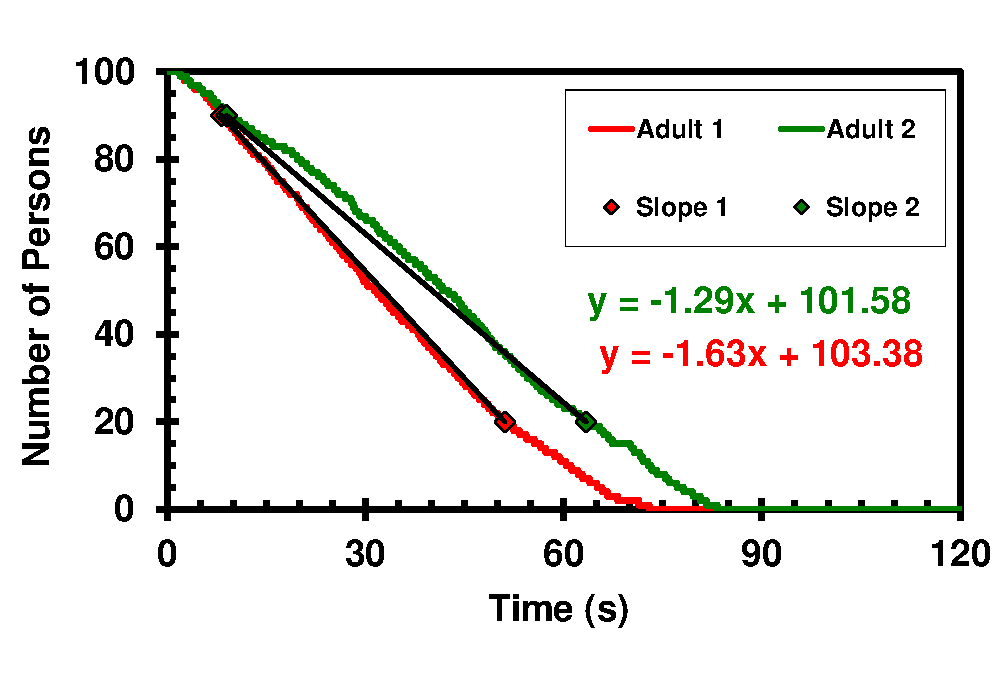
\includegraphics[clip=true,
  width=75mm]{FIGURES/CompTest4}} 
  \caption{FDS+Evac results for the IMO test case
  4.}\label{Fig_CompTest4}  
\end{figure}
%
%
\item \textbf{IMO 5} Response time: Verify that the humans start to
  walk according to a given uniform reaction time distribution.
  FDS+Evac passed the test.  FDS+Evac prints out the main properties
  of the agents, including their response and detection times,
  unimpeded walking velocities, main body diameters, motive force time
  constants $\tau_i$, and the initial positions.  This test is a
  little bit odd, because there is only 10 agents in the simulation so
  one can not get out any good statistics.  But one could see that
  each agent is starting accordingly to its randomly generated
  response time (both the response time and coordinates of the agent
  are printed out).  To test better the random distribution
  properties, the IMO test case 9 was used, where there are 1000
  agents.  Two different response time distributions were used, the
  day and night case ones of the IMO document~\cite{IMO07}.  These are
  both truncated logarithmic normal distributions.  The results of
  these tests are given in Fig.~\ref{Fig_IMOLogNormal}
%
\item \textbf{IMO 6} Rounding corners: Persons approaching a corner will
  successfully navigate around the corner without penetrating the
  boundaries.  FDS+Evac passed the test.  The social force model used
  for the movement of the agents does not allow the agents to go
  inside walls if the time step is small enough as it is in FDS+Evac
  for reasonable values of the model parameters.
%
\begin{figure}[!tb]
  \centerline{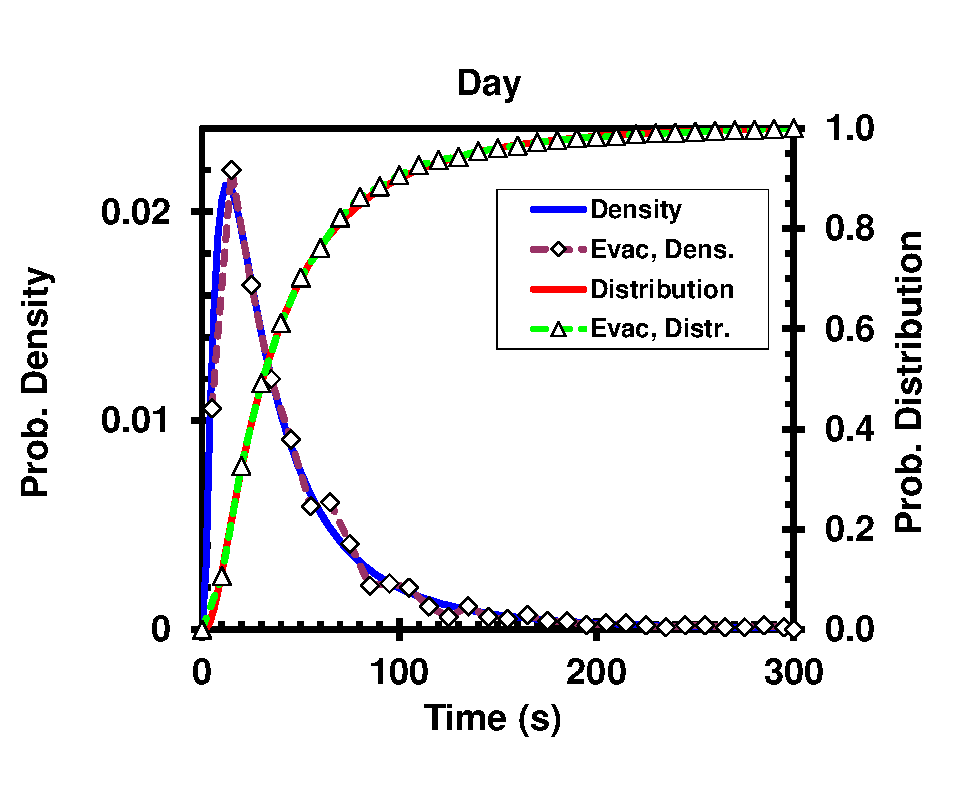
\includegraphics[clip=true,
  width=75mm]{FIGURES/LogNormal_IMO_circ1238_Day} ~  
  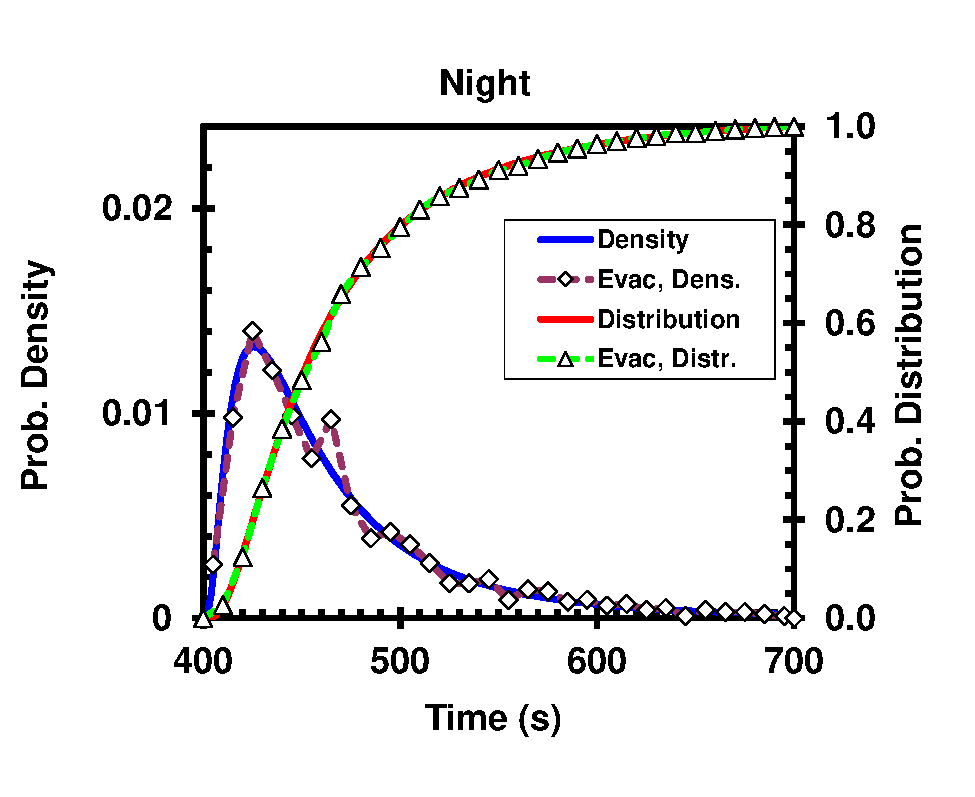
\includegraphics[clip=true,
  width=75mm]{FIGURES/LogNormal_IMO_circ1238_Night}}   
  \caption{A response time test for truncated logarithmic normal
  distributions.}\label{Fig_IMOLogNormal} 
\end{figure}
%
%
\item \textbf{IMO 7} Assignment of population demographics parameters:
  Distribute the walking speeds over a population of 50 people and
  show that the walking speeds are consistent with the distribution
  specified in the input.  FDS+Evac passed the test, see the test
  number IMO 5 above.  The obtained distribution parameters for a
  FDS+Evac run were: variance=0.041 (0.035), average=1.282 (1.295),
  median=1.290 (1.295), min=0.980 (0.970), max=1.620 (1.62), where the
  number in parentheses are the corresponding ones of the uniform
  distribution.  The same analysis was made for the IMO test case 9.
  This case has 1000 agents, so the statistical significance of the
  test for the distribution is much better.  The FDS+Evac results
  were: variance=0.036 (0.035), average=1.280 (1.295), median=1.280
  (1.295), min=0.970 (0.970), max=1.620 (1.62), so it can be said that
  FDS+Evac passed the test.
%
\item FED calculation: To test the implementation of Fractional
  Effective Dose (FED) concept~\cite{Purser03}, a simple one room
  geometry with no fire source and one agent in the middle of the room
  is used.  The agent is fixed at its initial position by setting the
  detection time large and by setting random noise of the movement
  equations to zero.  FDS point measurements of the gas concentrations
  and FED are placed at the position of the agent.  The room is
  initialized with different CO, CO${}_2$, and 0${}_2$ concentrations
  to test the overall FED calculation and each different component
  separately also.  The concentrations for the four different
  calculations were: (2, 0.1, 15)~\%, (0, 0, 12)~\% (0, 0.1, 21)~\%,
  and (3.43, 0.1, 21)~\% for the (CO${}_2$, CO, O${}_2$) volume
  fractions.  The room stays at the specified initial conditions,
  because there is nothing to generate a flow and also the initial
  random noise of FDS flow calculation is switched off.  The FDS+Evac
  output for the FED index of the agent is compared to a value
  computed using an external worksheet and the FDS point measurements
  for gas concentrations and for the FED index.  The results of the
  comparison are shown in Fig.~\ref{Fig_FED_Test}.  The results
  indicate that the FED calculation in FDS+Evac is implemented
  correctly (and that the ``FED'' point measurement output is also
  implemented correctly).
%
\begin{figure}[!tb]
  \centerline{\includegraphics[clip=true,
  width=100mm]{FIGURES/Test_Fds660Evac252_FED}} 
  \caption{A FED test.}\label{Fig_FED_Test}
\end{figure}
%
\item Unimpeded walking speed vs smoke density: Smoke reduces the
  walking speed due to the reduced visibility.  The prediction of this
  effect is tested in a 10~m long corridor geometry.  The unimpeded
  walking velocity for a smoke clear environment was set to 1.5~m/s.
  Four different calculations with soot densities of 0, 500, 1000, and
  1500 mg/m${}^\textrm{3}$ were performed.  Soot was introduced in the
  calculations as an initial mass fraction and the default initial
  random fluctuations of FDS were set to zero and no flow was
  introduced in the corridor so the constant initial conditions
  prevail the same during the simulation.  The result of this test is
  shown in Fig.~\ref{Fig_SmokeSpeedTest}.  The line labeled as
  ``Theory'' is the experimental correlation given by
  Eq.~(\ref{Eq_SpeedSmoke}).  The velocities of the agents in FDS+Evac
  simulations were calculated using the time needed to travel the last
  5~m in the corridor.  The results show that FDS+Evac accurately
  reproduces the anticipated reduction of walking speed.
%
\end{enumerate}
%
%
\begin{figure}[!tb]
  \centerline{\includegraphics[clip=true,
  width=100mm]{FIGURES/Fds660Evac252_Smoke_vs_Speed}}   
  \caption{A smoke vs speed test.}\label{Fig_SmokeSpeedTest}
\end{figure}
%


\section{Functional Verification}\label{Sec_FuncVeri}

\noindent For the functional verification required by IMO, a good
technical documentation should be enough.  The manual should set out
in a comprehensible manner the complete range of model capabilities
and inherent assumptions and give a guide to the correct use of the
capabilities.  It is left to the reader to decide if this manual, the
FDS+Evac web pages, and the open source code of the programme hosted
by Google Code\footnote{http://code.google.com/p/fds-smv/} satisfy
this criterion.


\section{Qualitative Verification}\label{Sec_QualVeri}

\noindent The qualitative features of FDS+Evac were tested using some
simple geometries to show that the agents behave like they are told in
the input and that their movement is qualitatively correct.  Most of
these simulations were performed in an evacuation trial mode,
\emph{i.e.}, there was no smoke or fire calculation present in the
simulations.  The effect of smoke and toxic gases on the decision
making processes of the agents were tested separately.  An interested
reader could download the input files of the test simulations from the
FDS+Evac web pages and rerun the cases.  This is especially true for
some cases, where the results can not be checked as numbers but one
should see ``by own eyes'' that the programme is working as it should.

%
\begin{enumerate}
%
\item \textbf{IMO 8} Counterflow -- two rooms connected via a
  corridor: Two 10$\times$10~$\mathrm{m^2}$ rooms are connected with a
  10~m long and 2~m wide corridor.  Initially there are 100 persons in
  the room 1 and the room 2 has 0, 10, 50, 100 persons and both rooms
  move off simultaneously.  The expected result is that the time the
  last person from the room 1 enters the room 2 increases as the
  number of persons in counterflow increases.
  
  FDS+Evac results were 50.01~s, 75.04~s, 106.85~s, and 136.14~s for
  the four cases, where there were 0, 10, 50, and 100 persons in the
  room 2, respectively.  FDS+Evac passed the test.
%
\item \textbf{IMO 9} Exit flow -- crowd dissipation from a large
  public room: A 30$\times$20~$\mathrm{m^2}$ public room with four
  1.0~m wide exits has 1000 persons.  Calculate the time the last
  person leaves the room.  Close two doors and repeat the calculation.
  The expected result is an approximate doubling of the time to empty
  the room.
  
  FDS+Evac passed the test.  The total evacuation times calculated
  using the default person properties were 220.74~s and 412.86~s when
  all four doors were open and when two doors were closed,
  respectively.  These times were 171.32~s and 322.85~s when the
  parameter value $\lambda_i$ is changed to 0.5.  Note that the flows
  through the 1.0~m wide doors were below 1.33~p/s when an ``Male''
  with the default parameter value $\lambda_i = 0.3$ were used (1.19
  and 1.23~p/s for the cases all doors open and two doors open,
  respectively).  For the parameter value $\lambda_i = 0.5$ the flows
  through the doors are slightly larger, 1.67 and 1.67 p/s.  See also
  the door flow test case in Sec.~\ref{Sec_CompOtherModels}.
%
\item \textbf{IMO 10} Exit route allocation: Populate a cabin corridor
  section with 23 persons and allocate the main exit for 15 persons
  and the secondary exit for 8 persons.  The expected result is that
  the allocated passengers move to the appropriate exits.
  
  FDS+Evac passed the test.  Note that this geometry needed some more
  effort to model, see the FDS+Evac input file on the FDS+Evac web
  pages for more information.  This is due to the fact that in order
  to model the test geometry rigorously the mesh cell sizes for the
  evacuation calculation meshes were 0.1~m in both the $x$ and $y$
  directions.  This is a little bit too fine mesh to construct the
  guiding floor flow fields for evacuation.  This problem does not
  arise if one is modelling the cabinets to have closed doors and
  enters the agents in to the calculation at the cabin doors.  This
  problem did not arise also when a grid cell sizes of 0.3~m was used
  both for the $x$ and $y$ directions.  Using this mesh the test
  geometry was modified just a little bit, the cabinet depths were
  5.1~m, not 5.0~m as specified in the IMO document.
%
\begin{figure}[!tb]
  \centerline{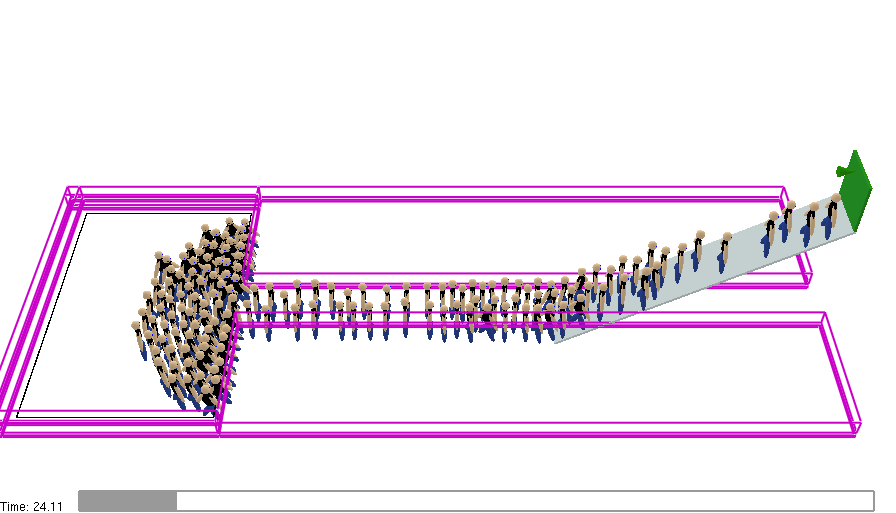
\includegraphics[clip=true,
  width=100mm]{FIGURES/CompTest11_24s}}   
  \caption{The IMO 11 staircase test case modelled by FDS+Evac using
    the \Timtt{EVSS} method.}\label{Fig_IMO11}
\end{figure}
%
\item \textbf{IMO 11} Staircase: A room populated with 150 persons is
  connected to a 2.0~m wide and 12~m long corridor which ends to a
  2~m wide stairs going upwards.  The expected result is that
  congestion appears at the exit from the room, which produces a
  steady flow in the corridor with the formation of congestion at the
  base of the stairs.
  
  FDS+Evac passed the test, if the user is giving reasonable input
  parameters for the definition of the staircase.  The \Timtt{\&EVSS}
  model for staircases was used, see Fig.~\ref{Fig_IMO11}.  The third
  staircase model (\Timtt{\&STRS} namelist) was not used, because it
  models whole staircase including landings, so it can not be used to
  model one single flight of stairs.
%
\begin{figure}[!tb]
  \centerline{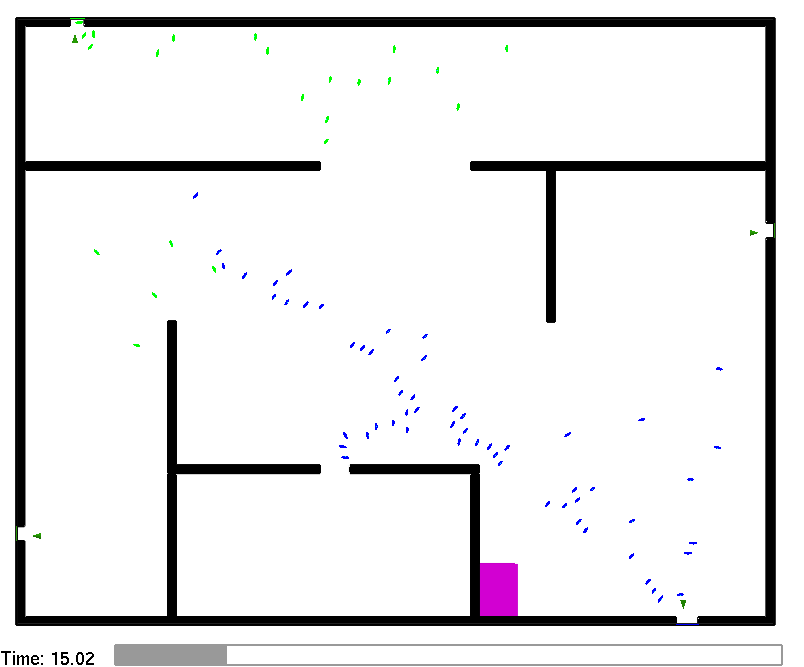
\includegraphics[clip=true,
  width=75mm]{FIGURES/DoorAlgo_A_15s} ~ 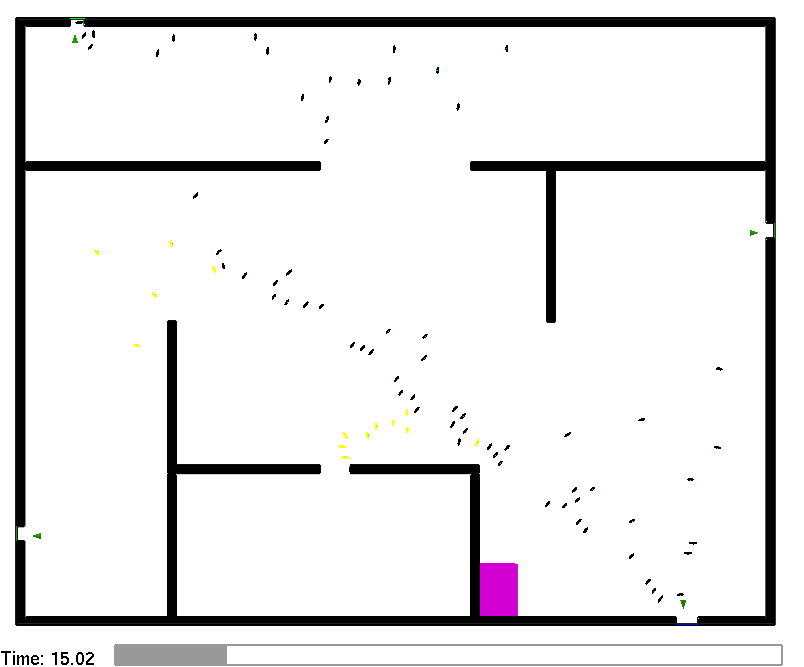
\includegraphics[clip=true,
  width=75mm]{FIGURES/DoorAlgo_B_15s}} 
  \caption{An exit door selection test without
    smoke.  On the left, agents are coloured according to their exit
    doors. On the right, they are coloured according to their current
    preference categories.}\label{Fig_ExitDoorNoSmoke}
\end{figure}
%
%
\item Decision making model without smoke: The verification of the
  exit door selection algorithm of FDS+Evac was tested using the
  geometry shown in Fig.~\ref{Fig_ExitDoorNoSmoke}.  On the left the
  the agents are coloured according to their target exit doors (blue:
  right bottom exit; green: top left exit) and on the right the
  colours of the agents mark the preference categories of the exit
  door selection algorithm (black: known visible door; yellow: known
  non visible door).  This test case has no smoke and as a result,
  agents use only the known doors (top left and bottom right ones).
  The doors on the left and right walls are not used, because they are
  not defined as ``known doors'' in the input.
  Figure~\ref{Fig_ExitDoorNoSmoke} verifies that the door selection
  algorithm works as intended when there is no smoke.  The agents
  first choose the nearest visible known door, if such exists.  If
  there are no visible doors, the agents choose the nearest non
  visible but known door; see the agents in the bottom left corner of
  the building.  Note however, that in the present version of
  FDS+Evac, the distance to the non visible doors is calculated along
  a straight line (L2 norm) through the internal walls.  In later
  versions, the algorithm may be changed to calculate the distance
  along the streamlines used to guide the agents towards the doors or
  using L1 norm.
%
\item Decision making model with smoke: The above test was modified by
  adding a fire that produces smoke to the building.  In
  Figure~\ref{Fig_ExitDoorSmoke} the visibility is shown at the height
  of the human eyes after 15~s from the ignition as a colour bar.  On
  the right the agents are coloured according to their target exit
  doors and on the right the colours of the agents mark the preference
  categories of the exit door selection algorithm.  Now the smokiness
  has changed the preferences.  First choices are still the doors with
  no smoke.  The input files for the exit selection tests are on the
  FDS+Evac web page an interested reader is able to reproduce the
  simulations and use Smokeview to see that the door selection
  algorithm is functioning like intended.
%
\begin{figure}[!tb]
  \centerline{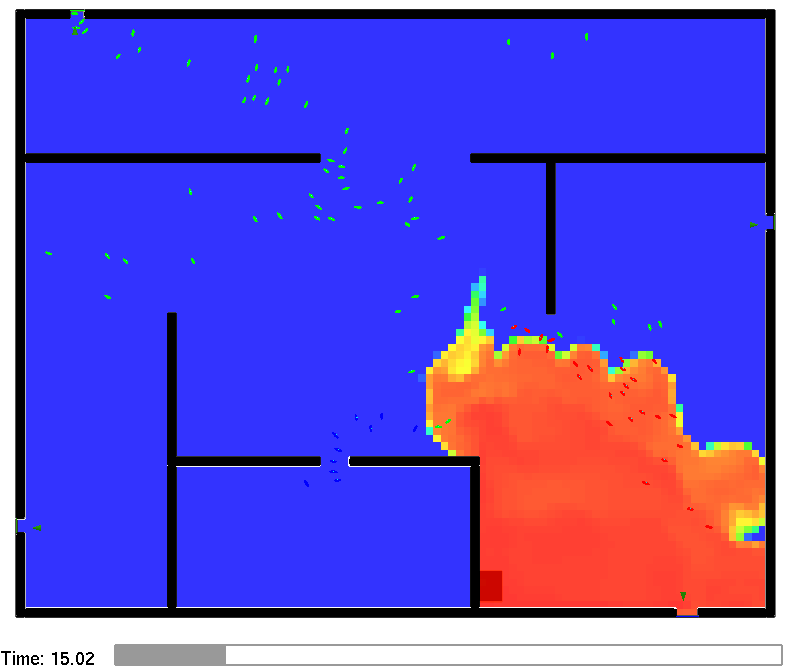
\includegraphics[clip=true,
  width=75mm]{FIGURES/DoorAlgo_C_15s} ~ 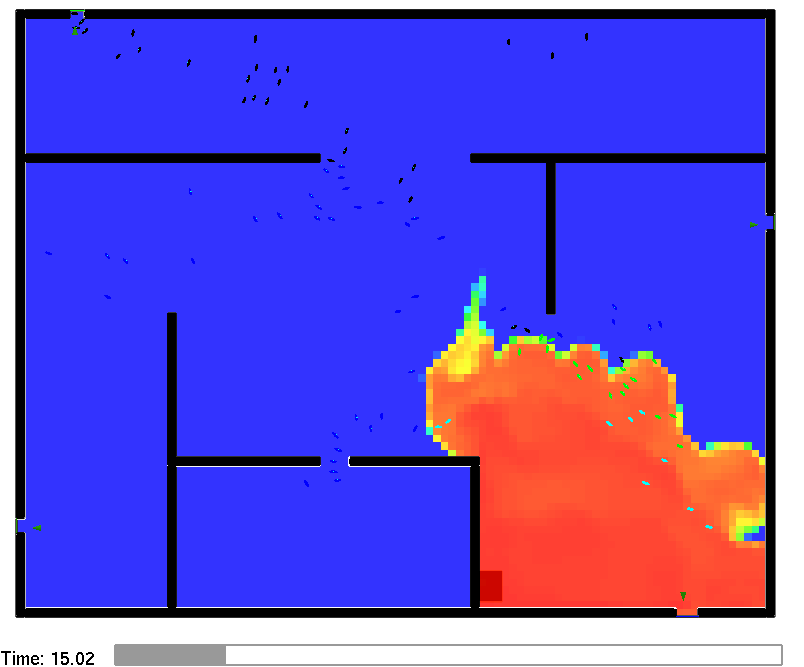
\includegraphics[clip=true,
  width=75mm]{FIGURES/DoorAlgo_D_15s}}  
  \caption{An exit door selection test with smoke.  On the left,
    agents are coloured according to their exit doors. On the right,
    they are coloured according to their current preference
    categories.  Shown is also the calculated visibility, where red
    indicates good and blue very bad visibility, see the colour
    bar.}\label{Fig_ExitDoorSmoke}
\end{figure}
%
%
\end{enumerate}
%


\section{Numerical Tests}\label{Sec_NumTest}

\noindent The numerical accuracy of the model depends on the time step
used to solve the equations of motion of the agents.  The time step
was chosen mainly by trial-and-error.  There are some convergence
checks made, see the paper by Korhonen \emph{et
  al}.~\cite{Korhonen08b}.  The properties of the exit selection
algorithm are examined in the paper by Ehtamo \emph{et
  al}.~\cite{Ehtamo2010}.

\clearpage

\newpage


\chapter{Model Sensitivity}\label{Sec_ModelSensi}


\section{Introduction}

\noindent This section concentrates on the effects of different input
parameters on the FDS+Evac results.  Especially the flows through
doors, corridors, and stairs are examined, because these are usually
the main bottlenecks of an evacuation event in a building.  This
section does not address the point if the chosen algorithms, numerical
methods, \emph{etc}.  are appropriate for the evacuation simulation or
not.  Only the sensitivity of the chosen algorithms and numerical
methods are examined and reported.  The tests presented here were done
in a ``fire drill'' mode, \emph{i.e.}, the egress processes were
simulated without any fire calculation.  Note that many of these
sensitivity studies are done using program version: FDS 6.0.0, Evac
2.4.1.  These results should also apply to the current version (FDS
6.5.3, Evac 2.5.2), because the basic movement algorithm has not been
changed and the (default) parameters of the movement models are the
same.


\section{Numerical Mesh Sensitivity}\label{Sec_GridSensi}

\noindent In principle, the movement algorithm of the agents described
in Sec.~\ref{Sec_BasisModel} does not have any underlying
computational mesh.  The algorithm is continuous in time and space.
But the implementation of the method in FDS+Evac introduces
computational meshes.  These meshes are used to define the geometry of
the calculation.  The most obvious mesh sensitivity issue is that the
spatial resolution of the obstructions, like doors, stairs,
\emph{etc.}, is the resolution of the underlying mesh.  The other,
subtler effect, is the way how the mesh resolution changes the flow
fields of the evacuation meshes, which are used to guide the agents
towards the exit doors.  In some cases, a finer grid does not always
mean a better guiding field for agents.  If the evacuation mesh
resolution is much less than half of the body dimension then one may
find some difficulties to obtain nice evacuation flow fields, see the
IMO test case 10 in Sec.~\ref{Sec_QualVeri} and the FDS+Evac web pages
for further details.


The FDS fire calculation mesh has effects on the evacuation
calculation via the smoke, toxic gas, temperature, and radiation level
calculation.  These quantities are taken to have constant values
inside each evacuation mesh cell.  How accurate are the predictions of
FDS for the fire products will, of course, depend on the FDS mesh
resolution.  See the FDS Technical Guide~\cite{FDS_Manual,
  FDS_VVGuide1, FDS_VVGuide2} for the effects of the mesh resolution
on the FDS fire calculation.  The evacuation calculation interpolates
the fire calculation results to the 2D evacuation meshes and the
evacuation mesh resolution will have an effect on the spatial accuracy
of this fire related information, but usually grid sizes are equal or
less than the dimensions of a human body and, thus, the accuracy of
the fire information in the evacuation meshes is fine enough for the
accuracy level of the evacuation calculation.  The default height,
where the toxic gas concentrations are taken, is 1.6~m above the floor
level.  Changing this value will have large effect on the FED index
calculation, of course.  If the user wants to be on the safe side,
then one should use height which is a little bit above the head
positions of the escaping humans, but this depends on the room
geometry, especially the height of the room.


There are many more important factors affecting the calculation of the
fire--agent interaction than the spatial resolution of the evacuation
and fire meshes, \emph{e.g.}, the production of CO and other toxic
gases depend largely on the user inputs.


\section{Human Parameter Sensitivity}\label{Sec_HumParSensi}

%
\begin{figure}[!tb]
  \centerline{ \includegraphics[clip=true,
    width=60mm]{FIGURES/Door_Geom} ~~~~~~~~   
    \includegraphics[clip=true,width=60mm]{FIGURES/CorrGeom2} }
  \caption{Test geometries used to calculate the specific flows through
    doors and corridors.\protect\hspace{200mm}}\label{Fig_Geoms}
\end{figure}
%

\noindent The agent movement algorithm of FDS+Evac has many
parameters.  Some of these are related to the physical description of
humans, like the body size, the mass, the walking speed, and the
moment of inertia.  The others are the parameters of the chosen
movement model, $\tau_i$, $\tau^z_i$, $\omega^0_i$, the parameters of
the social force, $A_i$, $B_i$, $\lambda_i$, and the parameters of the
contact force, $k_i$, $\kappa_i$, $c_d$.  To test the relative
importance of these parameters, Monte Carlo simulations were performed
to find the parameters, which have the greatest effect on specific
flows.  The calculations were done using Evac version 2.4.1.


Two different geometries were used in the Monte Carlo simulations, see
Fig.~\ref{Fig_Geoms}. One of the geometries was used to study the
flow through a narrow door and through a wide door and the other
geometry was used to study flows in a corridor using densities 1.0 and
2.0 persons per square metre.  There were 100 agents randomly located
at the $5 \times 5 ~\mathrm{ \textrm{m}^\textrm{2} } $ square in the
door flow calculations.  Corridor flow calculations had 96 or 192
agents inside the corridor depending on the density.  Thousand egress
simulation with different random initial properties were performed for
each of these four different cases.  The default ``Adult'' agent type
of FDS+Evac was used in the calculations, but in total twelve model
parameters, $A_i$, $B_i$, $\lambda_i$, $v^0_i$, $\tau_i$, $A_w$,
$B_w$, $\lambda_w$, $\omega^0_i$, $\tau^z_i$, $I^z_{i}$, $c_d$ were
varied $\pm 20~\%$ about their means using uniform distributions.  The
monitored output quantity was the specific flow in all cases and the
Spearman's rank correlation coefficients (RCC) were calculated for
these four cases and they are shown in Fig.~\ref{Fig_RCC}.

%
\begin{figure}[!tb]
  \centerline{\includegraphics[clip=true,
      width=75mm]{FIGURES/Collect_RCC_Fds600Evac241_Main1}  
      \includegraphics[clip=true,
      width=75mm]{FIGURES/Collect_RCC_Fds600Evac241_Main2} } 
  \caption{Rank correlation coefficients (RCC) for specific flows
    through doors and corridors.  Widths 0.8~m and 2.0~m were used for
    doors and human densities 1.0~$\mathrm{ \textrm{m}^\textrm{-2} } $
    and 2.0~$\mathrm{ \textrm{m}^\textrm{-2} } $ were used for
    corridors.\protect\hspace{200mm}}\label{Fig_RCC}
\end{figure}
%


It is seen from Fig.~\ref{Fig_RCC} that the parameters $A_i$, $B_i$,
$\lambda_i$, $v^0_i$, $\tau_i$, and $B_w$ have the largest impact on
the specific flows through doors and corridors. Thus, further
simulations were done to quantify these effects. Each of these six
parameters were varied separately and 100 simulations were done for
each discretely chosen value of the parameters.  Two different door
widths, 1.0~m and 2.0~m, were chosen to represent a narrow and a wide
door.  Corridor flow was calculated using a density of 2.0 persons per
square metre, because it is known that around this density the
specific flow has its maximum value.  For the density 1.0~persons per
square metre the corridor flow is mainly specified by the used
distribution for the unimpeded walking speeds, because at this density
the agents can move relatively independently of each others in the
corridor.  The results of these, in total almost 20~000 simulations,
are shown in Fig.~\ref{Fig_Door1}, where each marker represents the
average of 100 simulations.  Note that in FDS+Evac the initial
properties and positions of the agents are not deterministic, because
agents are randomly positioned, the parameters $R_d$, $v^0_i$, and
$\tau_i$, are sampled from random distributions and there are small
random forces in Eqs.~(\ref{Eq_motion}) and (\ref{Eq_rotmotion}).
Increasing the values of $A_i$ and $B_i$ increases the social force
which tries to keep agents apart from each other and, thus, the
specific flow for door geometry will decrease.  The corridor case has
a constant agent density.  Thus, these two parameters can not have an
effect through the density.  Larger social force, \emph{i.e.}, larger
$A_i$ and/or $B_i$, will make a forward walking person to reduce
his/her speed in order not to step on someone's heels, when the
anisotropy parameter, $\lambda_i$, is less than unity.  Increasing the
walking velocity will, of course, increase the specific flow.
Decreasing $\tau_i$, \emph{i.e.}, increasing the motive force to go
forward, increases specific flows quite rapidly for the door geometry.
This effect is not as pronounced in the corridor case, because there
is no free space in front of the agents to accelerate and also the
agents are already moving with some velocity whereas they are almost
standing and waiting their turn in front of the door.  The anisotropy
parameter of the social force, $\lambda_i$, controls how eager agents
are to push those who are in front of them.  When $\lambda_i$ is large
then agents are 'pushy'.  The effect of the wall force parameter $B_w$
is to modify the effective width of doors and corridors, thus,
increasing its value will make the effective width smaller and this
will decrease specific flows slightly.

%
\begin{figure}[!tb]
  \centerline{ \includegraphics[clip=true,
  width=50mm]{FIGURES/Collect_MainParametricStudies_Fds600Evac241_A}  
  \includegraphics[clip=true,
  width=50mm]{FIGURES/Collect_MainParametricStudies_Fds600Evac241_B} 
  \includegraphics[clip=true,
  width=50mm]{FIGURES/Collect_MainParametricStudies_Fds600Evac241_Lam} }  
  \centerline{ \includegraphics[clip=true,
  width=50mm]{FIGURES/Collect_MainParametricStudies_Fds600Evac241_v0}  
  \includegraphics[clip=true,
  width=50mm]{FIGURES/Collect_MainParametricStudies_Fds600Evac241_Tau} 
  \includegraphics[clip=true,
  width=50mm]{FIGURES/Collect_MainParametricStudies_Fds600Evac241_Bw} }
  \caption{Effects of different model parameters, $A_i$, $B_i$,
    $\lambda_i$, $v^0_i$, $\tau_i$, and $B_w$ on the specific flows
    through doors and corridors.  The corridor is 2.0~m wide, the
    agent density is 2.0~$\mathrm{ \textrm{m}^\textrm{-2} }$, and two
    different doors widths, 1.0~m and 2.0~m, are used.
    \protect\hspace{200mm}}\label{Fig_Door1}
\end{figure}
%


\section{Sensitivity of the Counterflow Algorithm}\label{Sec_CFSensi}

\noindent The agent movement algorithm to deal with counterflows in
FDS+Evac has many parameters.  To test the relative importance of
these parameters, Monte Carlo simulations were performed to find the
parameters, which have the greatest effect on specific flows.  The
calculations were done using FDS+Evac version 2.4.1.  In total fifteen
different parameters introduced in the collision avoidance algorithm
were varied.  The default values of the parameters are listed in
Table~\ref{Table_CFParameters}.


Two different geometries were used in the Monte Carlo simulations.
One was the door geometry shown in~\ref{Fig_Geoms}, where 1.0~m and
2.0~m wide doors were used.  There were 100 agents randomly located at
the $5 \times 5 ~\mathrm{ \textrm{m}^\textrm{2} } $ square in the door
flow calculations.  The other test geometry was the IMO test case 8
geometry, which has two 10$\times$10~$\mathrm{m^2}$ rooms connected by
a 10~m long corridor.  Corridor widths of 2.0~m and 4.0~m were used
and both rooms contained initially 100 agents.  The monitored output
quantity was the specific flow in the door geometry and in the
corridor case the entering time of the last agent from the left room
to the right room was recorded.  The Spearman's rank correlation
coefficients (RCC) were calculated for these four cases and they are
shown in Fig.~\ref{Fig_RCC_CF}.  Thousand egress simulation with
different random initial properties were performed for each of these
four different cases.  The default ``Adult'' agent type of FDS+Evac
was used in the calculations, but in total fifteen different
parameters of the counterflow model were varied about their means
using uniform distributions.

%
\begin{figure}[!tb]
  \centerline{\includegraphics[clip=true,
      width=75mm]{FIGURES/Collect_RCC_Fds600Evac241_CF1}  
      \includegraphics[clip=true,
      width=75mm]{FIGURES/Collect_RCC_Fds600Evac241_CF2} } 
  \caption{Rank correlation coefficients (RCC) for the emptying time
    through doors and corridors.  Door widths 1.0~m and 2.0~m were
    used for doors and widths of the corridors were 2.0~m and 4.0~m
    were used for corridors in the IMO test case 8
    geometry.}\label{Fig_RCC_CF}
\end{figure}
%    geometry.\protect\hspace{200mm}}\label{Fig_RCC}
%

%
\begin{figure}[!ht]
  \centerline{ \includegraphics[clip=true,
  width=50mm]{FIGURES/Collect_CFlow_PS_Ctau}\includegraphics[clip=true,
  width=50mm]{FIGURES/Collect_CFlow_PS_C1w}\includegraphics[clip=true,
  width=50mm]{FIGURES/Collect_CFlow_PS_Amincf} }  
  \centerline{ \includegraphics[clip=true,
  width=50mm]{FIGURES/Collect_CFlow_PS_Cncf}\includegraphics[clip=true,
  width=50mm]{FIGURES/Collect_CFlow_PS_Dv0}\includegraphics[clip=true,
  width=50mm]{FIGURES/Collect_CFlow_PS_Cv0} }  
  \centerline{ \includegraphics[clip=true,
  width=50mm]{FIGURES/Collect_CFlow_PS_C2w}\includegraphics[clip=true,
  width=50mm]{FIGURES/Collect_CFlow_PS_Ddf}\includegraphics[clip=true,
  width=50mm]{FIGURES/Collect_CFlow_PS_Cdf} }  
  \caption{Effects of different counterflow model parameters on the
    specific flows through doors and on the emptying time of the left
    room for IMO test case 8.  The corridor in the IMO case is 2.0~m
    wide, and two different doors widths, 1.0~m and 2.0~m, are
    used.}\label{Fig_CFParametric}
\end{figure}
%    \protect\hspace{200mm}}\label{Fig_CFParametric}
%

According to the RCC calculations some of the most important
parameters of the counterflow model were examined further by doing a
parametric studies, where different parameters were varied separately
and 100 simulations were done for each discretely chosen value of the
parameters.  Chosen geometries were the IMO test case geometry with
2.0~m wide corridor and door geometries with 1.0~m and 2.0~wide doors,
but these were not used for all the chosen model parameters.  Only
those parameter vs geometry cases were chosen where the RCC were
reasonably large.  The results are shown in
Fig.~\ref{Fig_CFParametric}, the markers are averages of the 100
simulations and standard deviations of the 100 simulations are shown
as error bars.  It can be seen that the chosen model for the collision
avoidance does not have a large effect on the flows through doors if
reasonably parameter values are used.  This is a good result, because
the intention was not to change the calculated flows through doors in
situations where there is no counter flow.  The earlier versions of
FDS+Evac were already doing a nice job in these situations.  For the
counterflow test case, IMO test 8, there can be some variations of the
results as the different parameters are varied, but these variations
are not generally large and in quite many cases are within the error
bars.


%
\begin{table}[!tb]
\begin{center}
\caption{The default values used for the short range collision
  avoidance algorithm in FDS+Evac.  Most of the values are just
  dimensionless factors but the two minimum relaxation time constants
  have dimensions.  The lables before the default values are the
  keywords that can be used on the \Timtt{PERS} namelist to change the
  values.}\label{Table_CFParameters}
\vspace{12pt}
\begin{tabular}{l|c|l} \hline \hline
$c_{df}$ & \Timts{CONST\_DF}=2.0  & Prefer agents same direction \\  % const_df 
$d_{df}$ & \Timts{FAC\_DF}=1.0  & Prefer agents same direction \\  % fac_df 
$c_{cf}$ & \Timts{CONST\_CF}=1.0  & Dislike agents opposite direction
  \\ %const_cf 
$d_{cf}$ & \Timts{FAC\_CF}=2.0  & Dislike agents opposite direction \\
                                % fac_cf 
$c_{1w}$ &  \Timts{FAC\_1\_WALL}=5.0 & Dislike directions towards
walls \\ % FAC_1_WALL 
$c_{2w}$ & \Timts{FAC\_2\_WALL}=10.0 & Dislike much if going if too
close to a wall \\ % FAC_2_WALL   
$c_{v0}$ &  \Timts{FAC\_V0\_DIR}=1.0 & If counterflow, prefer straight
ahead + right \\ %  FAC_V0_DIR   
$d_{v0}$ &  \Timts{FAC\_V0\_NOCF}=1.0 & Prefer v0 if no counterflow \\
                                % FAC_V0_NOCF 
$c_{ncf}$ & \Timts{FAC\_NOCF}=2.0 & Prefer v0 if no counterflow \\ % FAC_NOCF
$a_{min,cf}$ & \Timts{CF\_MIN\_A}=0.5 & If counterflow decrease social
force \\ % CF_MIN_A (N) 
$b_{min,cf}$ & \Timts{CF\_MIN\_B}=0.3 & If counterflow decrease social
force \\ % CF_MIN_B (m) 
$a_{w,cf}$ & \Timts{CF\_FAC\_A\_WALL}=1.0 & If counterflow decrease
social force \\ % CF_FAC_A_WALL  
$c_{\tau}$ & \Timts{CF\_FAC\_TAUS}=0.25 & If counterflow increase
motive force \\ % CF_FAC_TAUS 
$\tau_{min}$ & \Timts{CF\_MIN\_TAU}=0.1~s & If counterflow increase
motive force \\ % CF_MIN_TAU (s) 
$\tau_{min}^z$ & \Timts{CF\_MIN\_TAU\_INER}=0.05~s & If counterflow
increase motive force \\ \hline\hline 
% CF_MIN_TAU_INER (s)
\end{tabular}
\end{center}
\end{table}
%

Finally, it was decided to use the values given in
Table~\ref{Table_CFParameters} for the different parameters of the
counterflow model.  These parameters are probably not optimal for
counterflow, but they are at least working moderately good.  And by
changing them a little bit would not affect the outcome of the
calculation much.  For now the collision avoidance method is quite
short range and it does not try to model the way finding of real humans
in crowds too realistically.  The main idea of the model to enable
counter flow with reasonable high agent densities using a short range
collision avoidance.  The parameters which are used to avoid the
directions towards walls in the collision avoidance algorithm are
mainly chosen by trial and error.  It was checked that these were not
affecting the ``normal situation'' (no counterflow) and that in
counterflow situations the agents did not try to push too hard against
the walls in some different geometries.  Some other parameters were
chosen similarly by checking their possible ranges so that they did
not change the behaviour of FDS+Evac when there was no counterflow.
For example, if there are crowding but every agent is trying to go
more or less towards the same direction then the original $v_0$
direction is preferred.  For this kind of short range collision
avoidance method it is better that the agents are not changing their
behaviour in the ``normal situation''.  Optimizing the decision making
of an agent in general would need much more long range route planning
including ``vision''.  If there are dense crowds at the doors queueing
then the exit selection algorithm will mainly decide the outcome of
the overall evacuation event, not this kind of short range interaction
at the crowded doors, where there is no matter who is getting first
out on the overall performance of the evacuation situation.


\section{Summary}

\noindent One should be very careful when constructing the geometry,
where agents are moving.  One should use Smokeview to see the guiding
flow fields for the agents before making a full evacuation simulation.
To see the actual evacuation geometry and the flow fields, one should
do just a plain evacuation calculation without any fire meshes and see
the results in Smokeview.  One should especially check that there are
no smaller than about 0.7~m wide ``holes'' in the evacuation geometry,
because the agents need at least this wide exit paths.


The effect of the parameters in the agent movement algorithm,
Eqs.~(\ref{Eq_motion})--(\ref{Eq_motive_torque}), are understood well and
user should not usually use any other than the predefined person types
in FDS+Evac.  The default predefined person types use a value of 0.3
for the anisotropy parameter, $\lambda_i$, of the social force.  For
some applications the resulting specific flows may be considered to be
too low.  If this is the case then the user should use 0.5 as the
value of $\lambda_i$.  Note that in the earlier versions of the
programme the default value of this parameter was 0.5.

\clearpage

\newpage


\chapter{Model Validation}\label{Sec_ModelValid}


\section{Introduction}

\noindent Previous chapters are dealing on the fact that how the
implementation of the model worked as a computer code, \emph{i.e.} it
was tested that the programme is functioning as planned and it was
also considered how sensitive the model is to its input parameters.
These tests give confidence on how the model is working and how
accurate the model equations are solved numerically.  But these tests
do not necessary tell how well the model is modelling the actual
evacuation scenarios.  For this reason, the model predictions are
tested against experimental data from evacuation experiments and trial
evacuations in this chapter.  The model predictions are also compared
to the predictions of some other evacuation models.



\section{Comparisons with Test Data}

\noindent This chapter lists three test cases, where the FDS+Evac
predictions are compared to experimental data on human flows on
horizontal paths and stairs.  Most of the calculations were done using
FDS version 6.5.3 (Evac version 2.5.2).  The specific flows through
doors and corridors were done using FDS version 6.5.2 (Evac version
2.5.2). These should be valid for the version 6.5.3, because the
evacuation calculation should be the same (except some minor bug fixes
etc.) and these test cases are done in ``fire drill mode'', i.e., no
fire meshes are defined.


%
\begin{enumerate}
%
\item Specific flows through corridors: In the research of pedestrian
  flows, the dependence of the specific human flow rate on the human
  density is called as ``fundamental diagram''.  It shows how the
  specific flow first increases when the human density is increased,
  but then starts to decay as the density becomes high enough to
  hinder the walking.  In this test case, the specific flow rates
  given by the FDS+Evac code are compared to experimental walking
  velocities on horizontal floors in corridor geometry.  The geometry
  is shown in Fig.~\ref{Fig_Geoms}.  The corridor is modelled as a
  loop to avoid the effects of inflow and outflow boundary conditions.
  In Figure~\ref{Fig_CorrResults}, the predicted flow rates are
  compared against some experimental results for pedestrian traffic
  flows taken from Daamen's thesis~\cite{Daamen04}.  Note that almost
  all of the experimental information is obtained by studying
  bidirectional pedestrian flows, the results for unidirectional flows
  might give different results.  The FDS+Evac simulations were
  performed with two different parameter sets, labels ``default''
  refer to the defaults of FDS+Evac and labels ``fast'' refer to
  parameter sets, where $\lambda_i = 0.5$ is used.

  In Figure~\ref{Fig_CorrResultsAgentTypes} the calculated specific
  flows in the corridor geometry are shown for four predefined
  agent types in FDS+Evac.  Calculations were done using FDS version 6.5.2.

%
\begin{figure}[!tb]
  \centerline{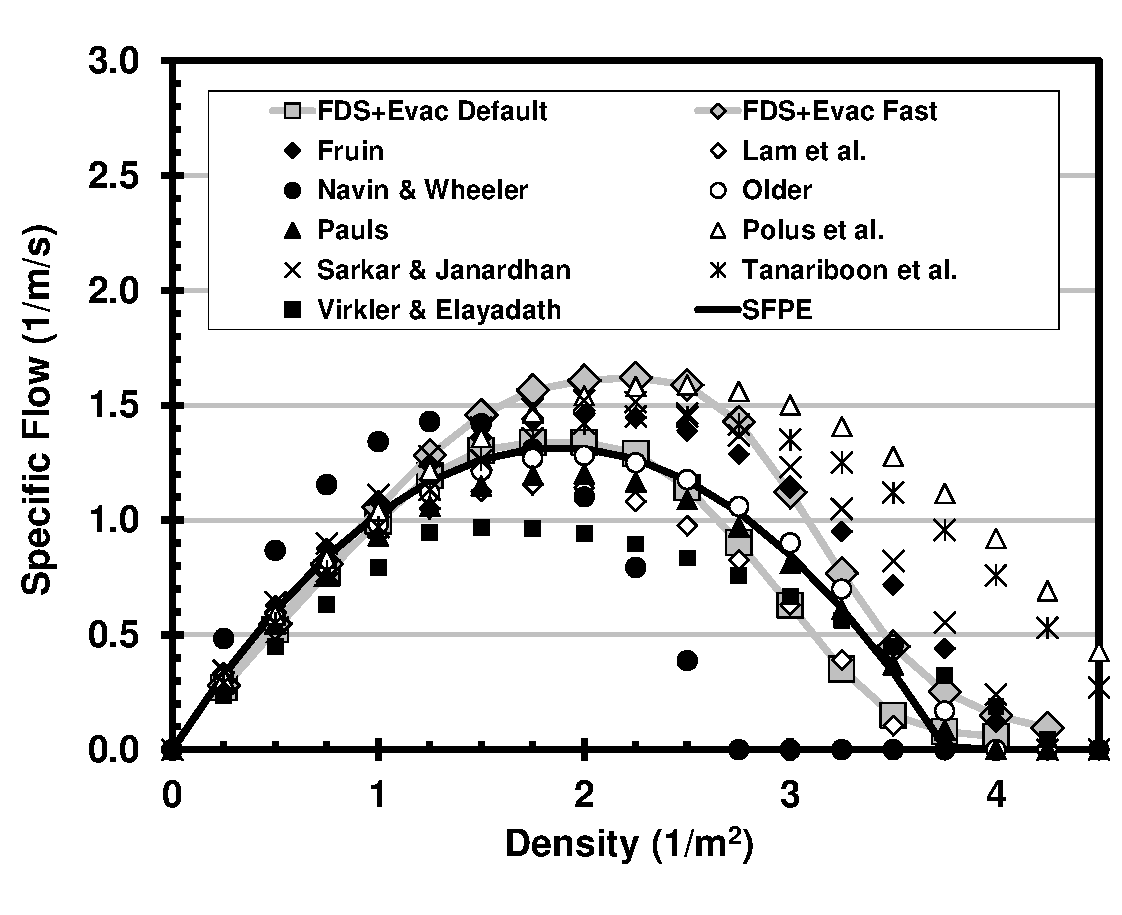
\includegraphics[clip=true,
  width=100mm]{FIGURES/CorrFlow_2m_Results}} 
  \caption{The specific flows in corridors, FDS+Evac results are
    compared to experimental values.}\label{Fig_CorrResults} 
\end{figure}
%

%
\begin{figure}[!tb]
  \centerline{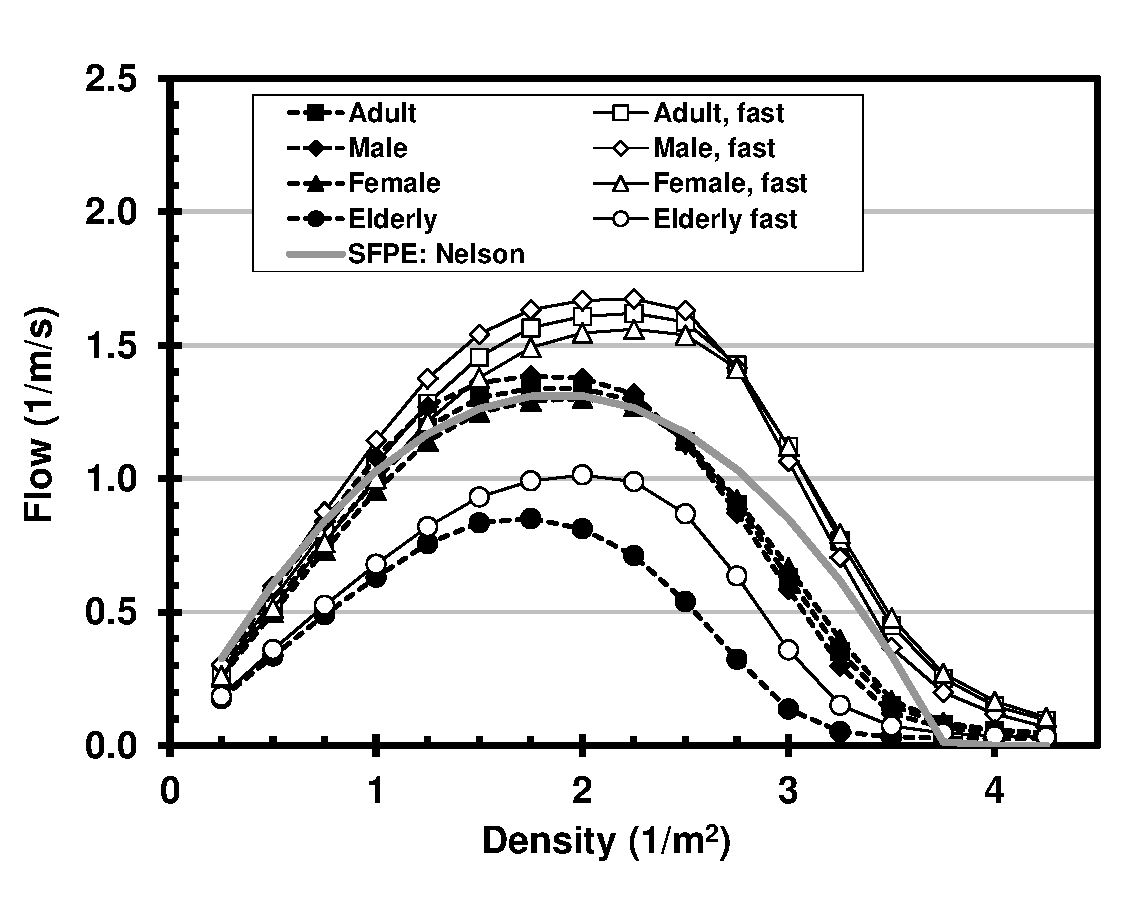
\includegraphics[clip=true,
  width=100mm]{FIGURES/CorrFlow_2m_Results_AgentTypes}} 
  \caption{The specific flows in corridors for the different default
    agent types of FDS+Evac.}\label{Fig_CorrResultsAgentTypes} 
\end{figure}
%

%
\begin{figure}[!b]
  \centerline{\includegraphics[clip=true,width=60mm]{FIGURES/PorrasKuva}}
  \caption{A snapshot from a FDS+Evac simulation showing the geometry
  of the staircase.}\label{Fig_StairGeom} 
\end{figure}
%

%
\item Staircase of an office building: An evacuation experiment at a
  large office building~\cite{Hostikka07b} was modelled using
  FDS+Evac.  Since the experiment was strongly focused on just one
  staircase, only this staircase was modelled.
  Figure~\ref{Fig_StairGeom} shows the geometry of the studied
  staircase.  The actual dimensions and door positions can be found in
  the experimental report~\cite{Hostikka07b}.  The experimental entry
  times of humans to the stair landings were taken as inputs to the
  simulations.  The standard adult person type of FDS+Evac was used in
  the simulations.  Two different values were used for the anisotropy
  parameter of the social force, $\lambda_i=0.3$ which is the default,
  and $\lambda_i=0.5$ which corresponds to more rapid egress.  The
  calculations for staircases were performed using all models for
  staircases available in FDS+Evac.
  

%
\begin{figure}[!tb]
  \centerline{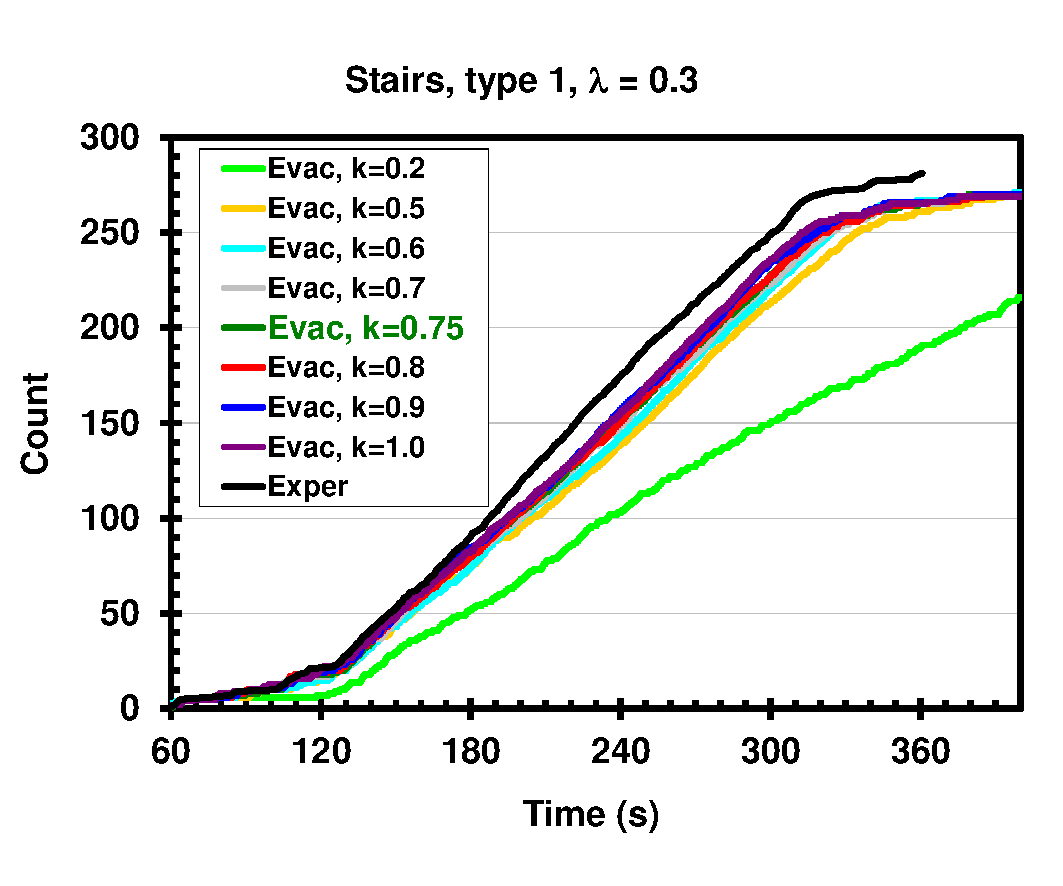
\includegraphics[clip=true,
    width=75mm]{FIGURES/OfficeStairs_Exper_vs_Evac_Type1_L0p3}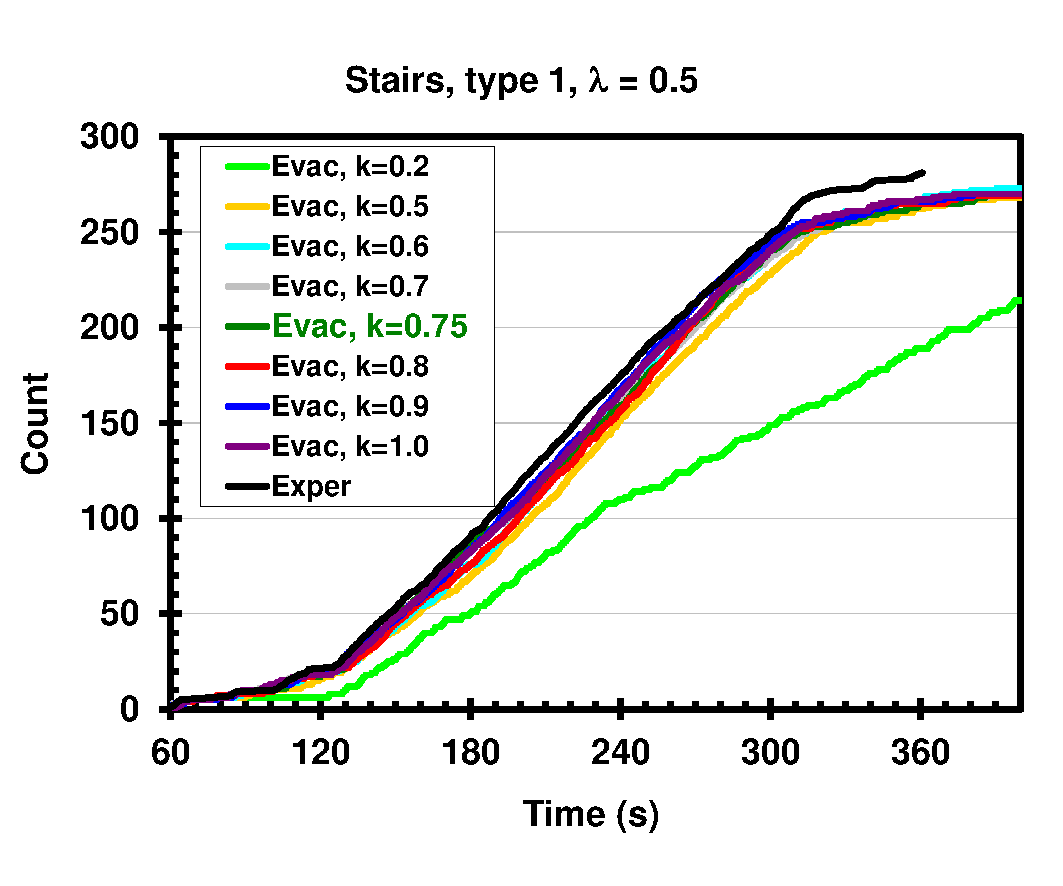
\includegraphics[clip=true,
    width=75mm]{FIGURES/OfficeStairs_Exper_vs_Evac_Type1_L0p5}}
  \caption{Comparison of FDS+Evac (staircase model type 1) and experimental
    observations of a staircase flow.  Values $\lambda_i=0.3$ (left)
    and $\lambda_i=0.5$ (right) for the anisotropy parameter of the
    social force are used.  Different curves correspond to the
    different values of the staircase speed reduction parameter
    $k$.}\label{Fig_StairType1}
\end{figure}
%

%
\begin{figure}[!tb]
  \centerline{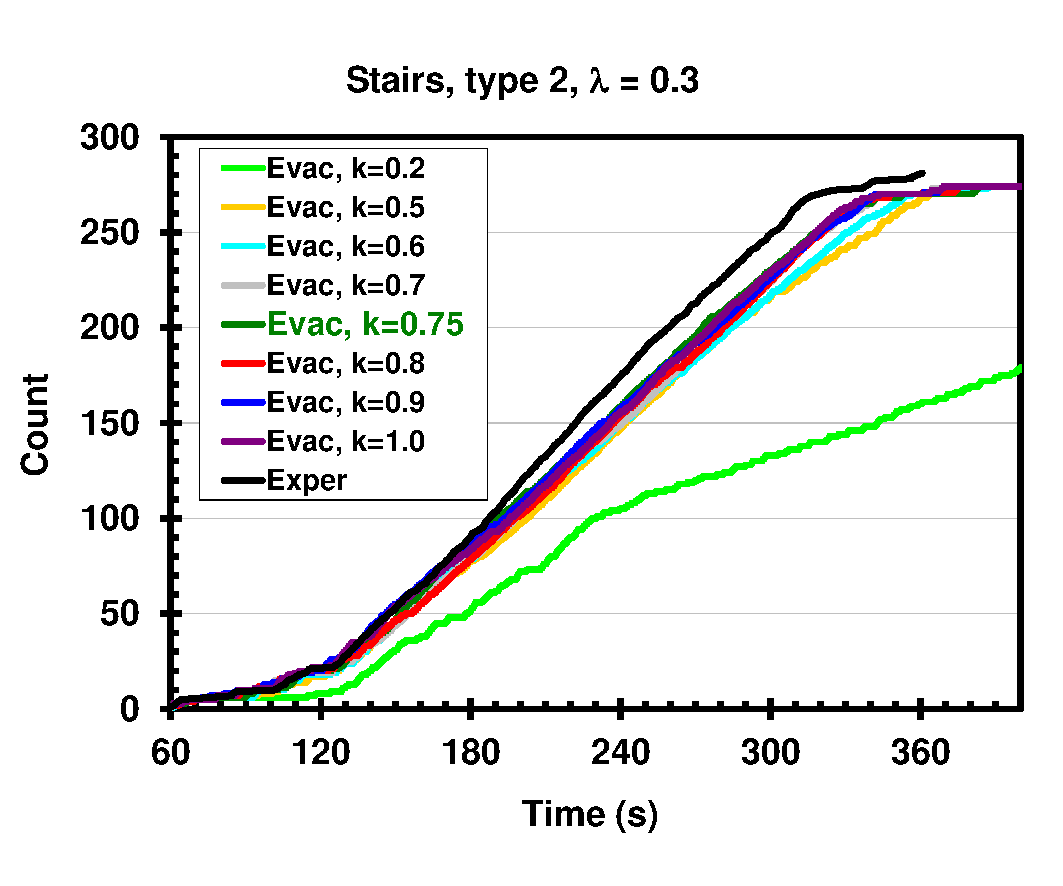
\includegraphics[clip=true,
  width=75mm]{FIGURES/OfficeStairs_Exper_vs_Evac_Type2_L0p3}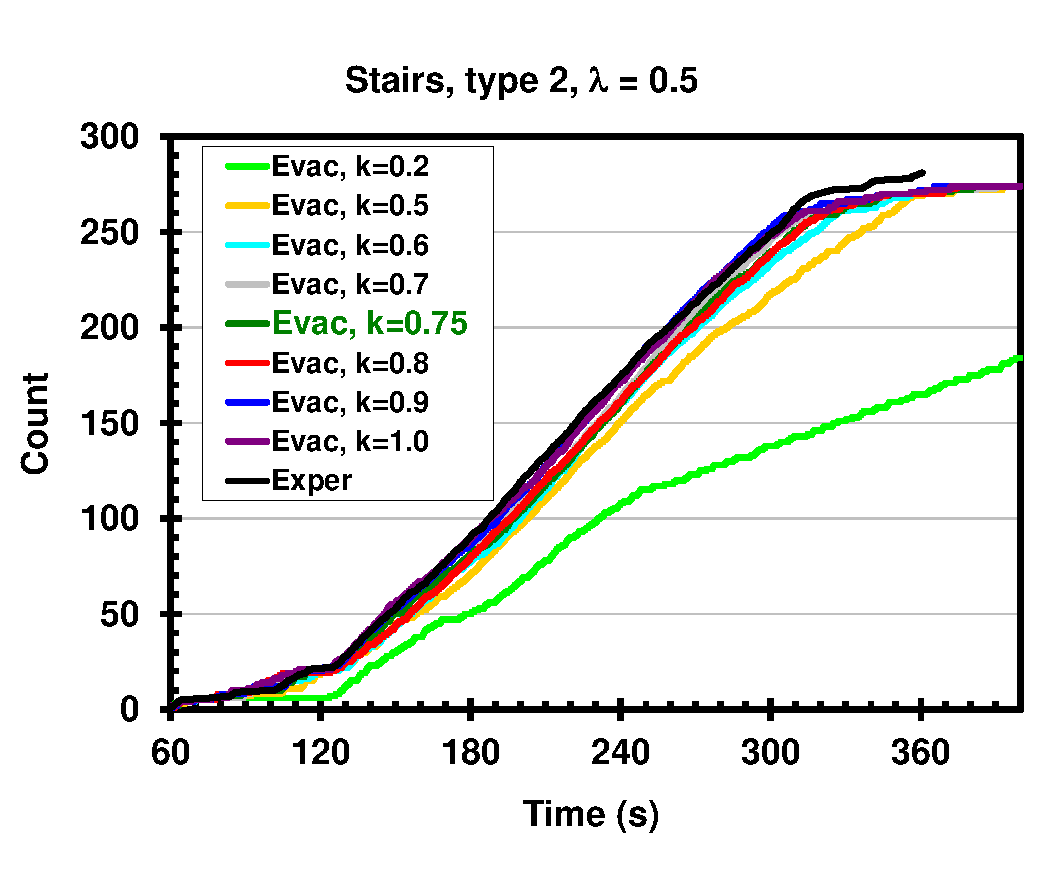
\includegraphics[clip=true,
  width=75mm]{FIGURES/OfficeStairs_Exper_vs_Evac_Type2_L0p5}}
  \caption{Comparison of FDS+Evac (staircase model type 2) and
    experimental observations of a staircase flow.  Values
    $\lambda_i=0.3$ (left) and $\lambda_i=0.5$ (right) for the
    anisotropy parameter of the social force are used.  Different
    curves correspond to the different values of the staircase speed
    reduction parameter $k$.}\label{Fig_StairType2}
\end{figure}

In Figure~\ref{Fig_StairType1} the experimental observations are
compared to the simulation results obtained by using the simple
staircase model (type 1).  This model is implemented using the
\Timtt{CORR} namelist, which is a crude model for stairs.  The
simulations were run several times corresponding to different values
of the staircase speed reduction parameter.  Reducing the unimpeded
walking speed by a factor $\gtrsim$0.5 seems to give a good agreement
with the observations.  Two different values of the anisotropy
parameter of the social force are used, $\lambda_i$=0.3 (the default
in FDS+Evac) and $\lambda_i$=0.5.  The $\lambda_i$=0.5 results seem to
reproduce the experimental findings better than the default value 0.3.
A speed reduction factor $\gtrsim$0.5 seems to produce more or less
quite constant flow at the exit door, \emph{i.e.}, at these speed
reduction values the stairs are feeding the front door fast enough.
For the case with $\lambda_i$=0.3 the specific flow in FDS+Evac
simulations is about 1.16~p/s/m and for the case with $\lambda_i$=0.5
the flow is about 1.30~p/s/m at the final exit door (speed factor
0.75).  The observed flow rate at the final exit door (width 1.07~m)
was 1.35 p/s in the experiment.
% Numbers are for fds6.5.3Evac2.5.2
%

%
\begin{figure}[!tb]
  \centerline{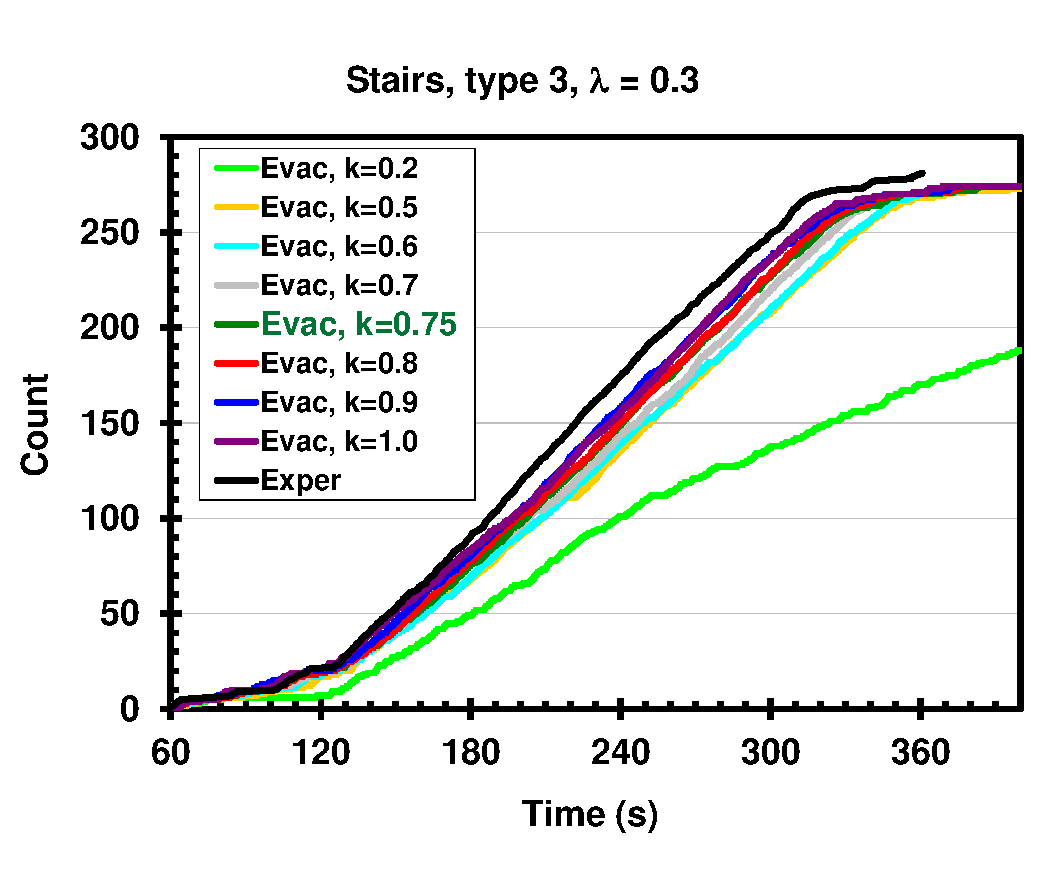
\includegraphics[clip=true,
    width=75mm]{FIGURES/OfficeStairs_Exper_vs_Evac_Type3_L0p3}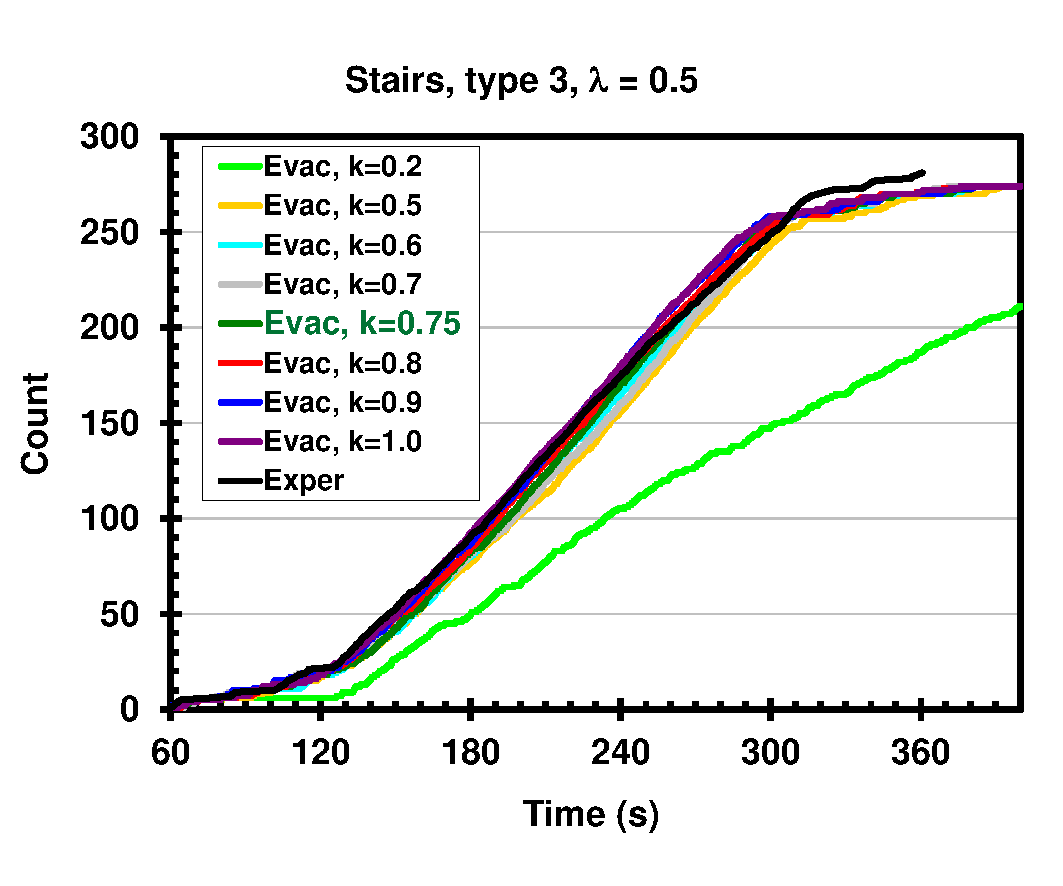
\includegraphics[clip=true,
    width=75mm]{FIGURES/OfficeStairs_Exper_vs_Evac_Type3_L0p5}}
  \caption{Comparison of FDS+Evac (staircase model type 3) and
    experimental observations of a staircase flow.  Values
    $\lambda_i=0.3$ (left) and $\lambda_i=0.5$ (right) for the
    anisotropy parameter of the social force are used.  Different
    curves correspond to the different values of the staircase speed
    reduction parameter $k$.}\label{Fig_StairType3}
\end{figure}

The results using a more sophisticated way of defining staircases
(type 2) are compared to the observed values in
Fig.~\ref{Fig_StairType2}.  In these simulations, the stairs are
modelled as inclines (\Timtt{EVSS} namelist), where agents move at
reduced speed.  Reducing the unimpeded walking speed by a factor
$\gtrsim$0.7 seems to give a good agreement with the observations.
Note that there exists some queuing at the final exit door opening to
the street in the experiment and this is also seen in the simulation
results, when the speed reduction parameter is not too low.  For the
case with $\lambda_i$=0.3 the specific flow is about 1.17~p/s/m and
for the case with $\lambda_i$=0.5 the flow is about 1.30~p/s/m at the
final exit door (speed factor 0.75).  Similar flows were also obtained
when using the simple staircase model (type 1).  When a speed
reduction factor $\gtrsim$0.7 is used seems to produce more or less
quite constant flow at the exit door, \emph{i.e.}, at these speed
reduction values the stairs are feeding the front door fast enough.
% Numbers are for fds6.5.3Evac2.5.2
%


The results using a most sophisticated way of defining staircases
(type 3) are compared to the observed values in
Fig.~\ref{Fig_StairType3}.  In these simulations, the whole stairs are
modelled as one single object using \Timtt{STRS} namelist, where
agents move at reduced speed on stairs flights and normal speeds on
landings.  Reducing the unimpeded walking speed by a factor
$\gtrsim$0.6 seems to give a good agreement with the observations.
Note that there exists some queuing at the final exit door opening to
the street in the experiment and this is also seen in the simulation
results, when the speed reduction parameter is not too low.  For the
case with $\lambda_i$=0.3 the specific flow is about 1.18~p/s/m and
for the case with $\lambda_i$=0.5 the flow is about 1.40~p/s/m at the
final exit door (speed factor 0.75).  Similar flows were also obtained
when using the other staircase models.  When a speed reduction factor
$\gtrsim$0.6 is used seems to produce more or less quite constant flow
at the exit door, \emph{i.e.}, at these speed reduction values the
stairs are feeding the front door fast enough.
% Numbers are for fds6.5.3Evac2.5.2
%

\begin{figure}[!tb]
  \centerline{\includegraphics[clip=true,
  width=120mm]{FIGURES/Library_Kuva2}} 
  \caption{A snapshot from a FDS+Evac simulation shows the geometry of
    the FDS+Evac model for the second floor of the public
    library.}\label{Fig_Kirjasto}
\end{figure}

%
\item Public library: An observed evacuation experiment of a public
  library~\cite{Hostikka07b} was simulated to study the capability to
  predict the entire movement phase of the evacuation, consisting of
  movement inside the floor, queueing to the staircase and finally
  movement through a narrow staircase to the exit.  The simulation
  geometry and the initial positions of the persons are shown in
  Fig.~\ref{Fig_Kirjasto}.  As the majority of persons in the building
  used the north exit door, the main results are for this door.  Shown
  are also the results for the west door, where about 50\% of the
  people originated from the first floor.  In the simulations, only
  the second floor of the building was simulated and people
  originating from the first floor were placed into the second floor.
  The north door was the only door with observed crowding.

%
\begin{figure}[!tb]
  \centerline{
    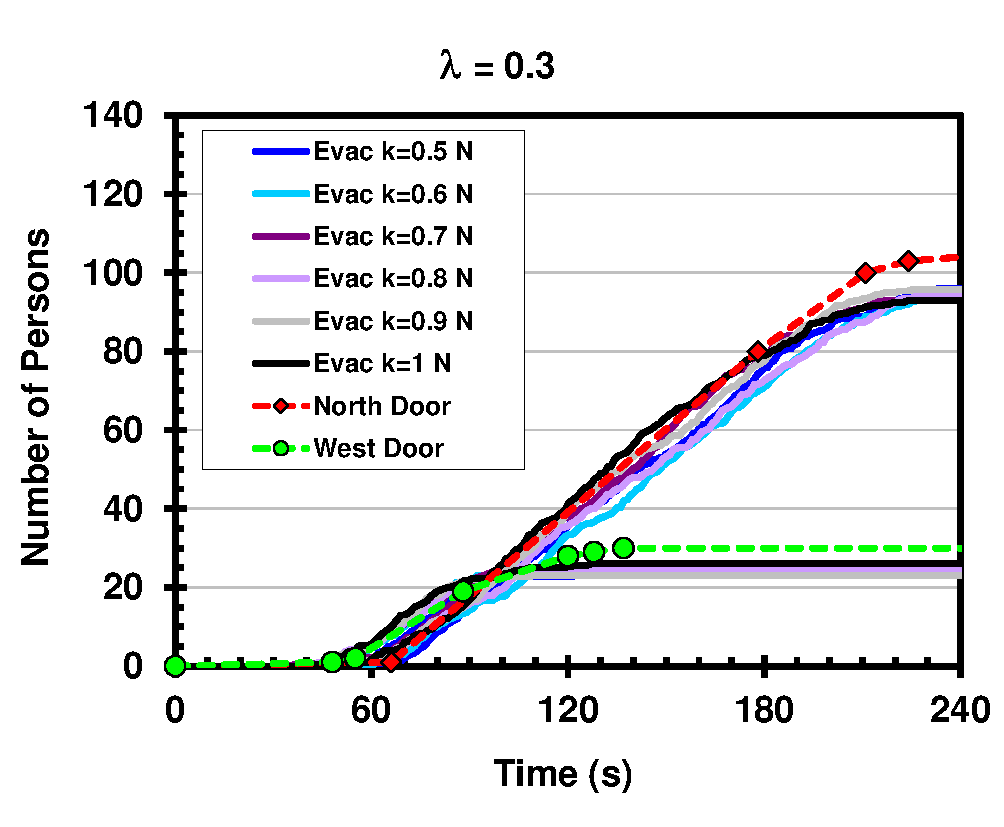
\includegraphics[clip=true,
    width=75mm]{FIGURES/HUT_Library_Results_L0p3} 
    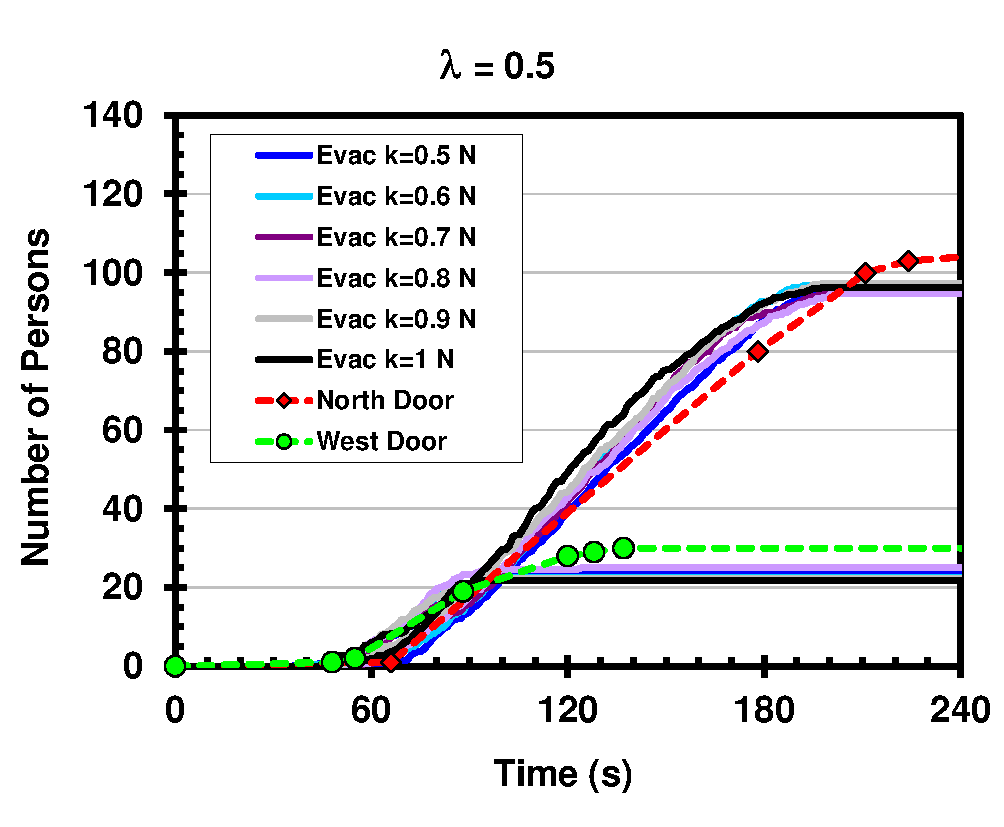
\includegraphics[clip=true,
    width=75mm]{FIGURES/HUT_Library_Results_L0p5} 
  }
  \caption{Comparison of FDS+Evac simulation results and observations
    at the north and west doors of the public
    library.}\label{Fig_KirjastoResults}
\end{figure}
  
The decision making processes were not modelled.  Instead, the people
were allocated for the north and west doors according to the ratio
observed in the experiment.  The simulations were performed using the
standard agent type ``Adult'' and the stairs at the north and west
doors were modelled using the \Timtt{EVSS} namelists.  The
pre-movement times were generated from symmetric triangular
distribution with mean of 41~s and lower and upper limits of 11~s and
71~s, respectively.  A comparison of the simulated and experimentally
observed flows is shown in Fig.~\ref{Fig_KirjastoResults}.  On the
left hand side the results of the simulations with default parameters
is shown and on the right hand side the anisotropy parameter of the
social force is increased from the default value ($\lambda_i=0.3$) to
$\lambda_i=0.5$.  The calculations have been done using different
values for the speed reduction factor in stairs, values 0.5, 0.6, 0.7,
0.8, 0.9, and 1.0 were used.  As can be seen, the predicted flow rates
agree in general with the experiments.  The default value for
$\lambda_i$ gives a little smaller flows than the experiment whereas
the increased value for $\lambda_i$ produces a little bit too fast
flows.  From these results it can be argued that a moderate, say
0.7--0.8, speed reduction factor in stairs seems to produce good
results.  For the west door, the results reflect the goodness or
badness of the assumed pre-movement time distribution because the flow
rate through the door is quite small.  For the north door, the
simulation is very relevant, because the flow rate is mainly
determined by the geometry and the crowd dynamics during the queueing
process.
%
%
\end{enumerate}
%

%Case 1: RI Nightclub: ToDo

%Case 2: Theatre at Tampere, Finland: ToDo

% ToDo: stair flows vs correlations

% TODO: Isobe et al counterflow

% TODO: Duisburg experiment for counterflow


\section{Comparisons with Other Evacuation
  Models}\label{Sec_CompOtherModels} 

\noindent The FDS+Evac model is compared here to other evacuation
models using four different geometries.  The FDS+Evac results and
corresponding input files are on the FDS+Evac web pages and some of
these cases are also discussed in the summary report of the FDS+Evac
development project~\cite{Hostikka07a}.  These calculations were done
using FDS+Evac version 2.5.2.
%


%
\begin{figure}[!b]
  \centerline{\includegraphics[clip=true,
  width=120mm]{FIGURES/SportHallGeom}} 
  \caption{The geometry of the studied sports hall.  The open grey
    area shows, where the agents are at the start of the simulations.
    The red rectangle shows the fire location, which is close to door
    3 and, thus, this door is not used.}\label{Fig_SportGeom}
\end{figure}
%

\begin{enumerate}
%
\item Sports hall: FDS+Evac simulations were compared to
  Simulex~\cite{Simulex96, Thompson95a, Thompson95b, Thompson03}
  simulations in a sports hall shown in Fig.~\ref{Fig_SportGeom}.
  The hall was previously analysed by Paloposki \emph{et
    al.}~\cite{Paloposki02}.  The sports hall is used to practice
  different kind of sports.  There are no spectator stands in the hall
  and neither are there any social spaces like showers.  People enter
  the hall through the main entrance (``Door 1''), which is 1.8~m wide
  double leaf door.  Doors 2 and 3 are 4.0~m wide two leaf doors and
  doors 4 and 5 are 0.9~m wide single leaf doors.  It is assumed that
  a fire starts close to door 3 (the shaded rectangle in
  Fig.~\ref{Fig_SportGeom}) so that this door cannot be used for
  egress.  235 persons use the closest door (``Door 5''), 130 persons
  use the main entrance (``Door 1''), 60 persons door 2, and 75
  persons use door 4.  These numbers are user input, so the door
  selection algorithm of FDS+Evac is not used in this example case,
  because also in the Simulex simulation the usage of the doors was
  described before the simulation.  Persons are initially located at
  the east end of the hall in an area of 20$\times$25~$\mathrm{m^2}$
  (the open rectangle in Fig.~\ref{Fig_SportGeom}).  Two different
  reaction time scenarios were considered, one having a normal
  distribution with a standard deviation of 15~s and mean 60~s, and
  the other one having a log-normal distribution (median 75~s,
  standard deviation of the logarithm of reaction time was 0.7).
  Actually, the log-normal distribution was approximated by two
  uniform distributions, because the version of the Simulex, which was
  used, did not support log-normal distributions for the reaction
  time, see the report by Paloposki~\cite{Paloposki02} for further
  details.

  %
  \begin{figure}[!tb]
    \centerline{\includegraphics[clip=true,
      width=100mm]{FIGURES/SportHall_Results_FDS660_Evac252}}
    \caption{The comparison of FDS+Evac to Simulex in a sport hall
      case.  The average of five different simulations are shown for
      each case.}\label{Fig_SportResults}
  \end{figure}
  %

  
  The results of the simulations are shown in
  Fig.~\ref{Fig_SportResults}.  The FDS+Evac simulations were done
  using 0.5~m mesh cell division, so the door widths were fitted to
  this resolution.  The door widths used in the simulations were 1.0~m
  (doors 4 and 5), 4.0~m (door 2), and 1.5~m for the main entrance.
  Since both FDS+Evac and Simulex are modelling human egress as a
  stochastic process, the presented results were collected from five
  different runs per case.  The FDS+Evac and Simulex results agree
  very well for the log-normal reaction time case, but for the other
  two cases the results differ somewhat.  These differences arise due
  to the ``Door 5'', which is only 1.0~m wide in the FDS+Evac
  simulations, but through which 235 persons escape.  The flow through
  this door is larger in Simulex than in FDS+Evac.  The flow through
  this door in the FDS+Evac simulations is 1.29~p/s for the case,
  where normal distribution was used for the reaction times and the
  default values for the anisotropy parameter $\lambda_i$ is used
  (``Evac2'').  If a value of 0.5 is used for the anisotropy parameter
  $\lambda_i$ the flow is increased to 1.67~p/s (``Evac'').  The other
  doors are not as crowded and there the capacities of the doors do
  not show up as much.
  % Numbers are for fds6.5.3Evac2.5.2

%
\begin{figure}[!tb]
  \centerline{\includegraphics[clip=true,
  width=80mm]{FIGURES/OpenFloorGeom}} 
  \caption{The geometry of the open floor office test
    case.}\label{Fig_OpenFloorGeom}
\end{figure}
%

%
\begin{figure}[!b]
  \centerline{\includegraphics[clip=true,
  width=100mm]{FIGURES/Office_Results_FDS660_Evac252}} 
  \caption{The comparison of FDS+Evac to Simulex in an open floor
    office case.}\label{Fig_OpenFloorResults} 
\end{figure}
%

\item Open floor office: This test geometry was an open floor office,
  whose floor plan is shown in Fig.~\ref{Fig_OpenFloorGeom}.  The
  floor has dimensions of 40$\times$40~$\mathrm{m^2}$ and there are
  initially 216 persons on this floor.  The properties of these agents
  were assumed to be as the ``Office Staff'' category in the Simulex
  model and the reaction times of the agents were assumed to follow a
  normal distribution with mean of 90~s and standard deviation of
  11~s.  There are three stairs located at the central core of the
  building.  The widths of the doors opening to the stairs are 1.2~m.
  In total seven different egress scenarios were simulated, covering
  the cases where all stairs are in use, one stair is blocked and a
  case where two stairs are blocked.
  
  The results of FDS+Evac simulations are compared to results of
  Simulex simulations in Fig.~\ref{Fig_OpenFloorResults}.  Only when
  two exit doors were blocked, queues were formed at the door.  For
  two or three operational doors the main form of the evacuation
  curves arise from the reaction time distribution.  The FDS+Evac and
  Simulex results are quite similar, but it can be noticed that
  FDS+Evac predicts somewhat longer evacuation times than Simulex.
  This can once again be traced back to the fact that FDS+Evac with
  the default value of 0.3 for the anisotropy parameter of the social
  force gives little bit smaller specific flows at doors than Simulex.
  It should be mentioned, that in the FDS+Evac simulations, the
  initial (random) positions of agents do not change between different
  door scenarios (see Fig.~\ref{Fig_OpenFloorGeom}), whereas in
  Simulex runs the random initial positions are different in each
  calculation.  This explains why the Simulex results have larger
  scatter in the cases where a certain number of doors are
  operational.\vspace{\fill}


%
\begin{figure}[!tb]
  \centerline{~~~\includegraphics[clip=true,
  width=130mm]{FIGURES/AssemblySpaceGeom}} 
  \centerline{\includegraphics[clip=true,
  width=120mm]{FIGURES/AssemblySpace_Simulex_60s}} 
  \caption{A snapshot from (a) FDS+Evac, (b) Simulex
    calculation.}\label{Fig_AssemblySnapshots} 
\end{figure}
%

\pagebreak[3]
%
\item Assembly space: The third test case is a large fictitious
  assembly space having dimensions of 50$\times$60~$\mathrm{m^2}$ and
  1000 people initially inside.  There is only one 7.2~m wide corridor
  leading to the exit.  The geometry is shown in
  Fig.~\ref{Fig_AssemblySnapshots}.  The FDS+Evac results (``Evac2'')
  are compared to those of Simulex (``Simulex'') and
  buildingExodus~\cite{Exodus3} (``Exodus'') in
  Fig.~\ref{Fig_AssemblyResults}.  Note, that the FDS+Evac simulations
  were also done using parameters describing more rapid egress
  (labels ``Evac''), where the value of the anisotropy
  parameter of the social force, $\lambda_i$, had a value of 0.5
  instead of the default 0.3.
  
  Considerable differences are shown between the results of FDS+Evac
  and the results of Simulex and buildingExodus programmes.  These
  differences can be traced back to the motion of the agents in the
  corridor, see Fig.~\ref{Fig_AssemblySnapshots}.  Simulex and
  buildingExodus are not using the whole width of the corridor
  efficiently, when the simulations are done using the default values
  and standard input.  (An advanced user of these codes might be able
  to get different results by using some additional features.)  The
  results of FDS+Evac model look more realistic.  The calculated
  specific flows (1/p/m) are: Simulex 0.47, Exodus 0.69, FDS+Evac 1.23
  ($\lambda_i=0.3$), and 1.57 ($\lambda_i=0.5$).
  % Numbers are for fds6.5.3Evac2.5.2
  
  In Figure~\ref{Fig_AssemblyResults} also shown are the results of
  the simulations for a case, where there is no corridor at all,
  \emph{i.e.}, there is just one 7.2~m wide exit door located at the
  wall of the room.  In this case, the agreement between the different
  evacuation programmes is much better.  The calculated specific flows
  (1/p/m) are: Simulex 1.59, Exodus 1.95, FDS+Evac 1.62
  ($\lambda_i=0.3$), and 2.01 ($\lambda_i=0.5$).
  % Numbers are for fds6.5.3Evac2.5.2

%
\begin{figure}[!tb]
  \centerline{\includegraphics[clip=true,
  width=100mm]{FIGURES/AssSpace_Results_FDS660_Evac252}} 
  \caption{The comparison of FDS+Evac to buildingExodus
    and Simulex in an assembly space.}\label{Fig_AssemblyResults}
\end{figure}
%
%
%
\begin{figure}[!b]
  \centerline{\includegraphics[clip=true,
  width=100mm]{FIGURES/DoorFlow_Results}} 
  \caption{The specific flows through doors.}\label{Fig_DoorResults}  
\end{figure}
%
%
\begin{figure}[!b]
  \centerline{\includegraphics[clip=true,
  width=100mm]{FIGURES/DoorFlow_Results_FdsEvacTypes}} 
  \caption{The specific flows through doors for the predefined
    FDS+Evac agent types. Labels ``fast'' refer to agent types, where
    the social force parameter $lambda$ is 0.5.}\label{Fig_DoorResultsHumanTypes}  
\end{figure}
%

%
\item Specific flows through doors: The fourth test geometry is the
  same one as used in Sec.~\ref{Sec_HumParSensi} for human
  parameter sensitivity studies and it is shown on the left hand side
  in Fig.~\ref{Fig_Geoms}.  This geometry is commonly used in the
  literature to calculate the specific flows through doors.  In the
  test, there are 100 agents randomly located at the
  5$\times$5~$\mathrm{m^2}$ square in front of the door.  In
  Figure~\ref{Fig_DoorResults}, the results of FDS+Evac simulations
  for specific flows through doors are compared to simulation
  programmes Simulex and MASSEgress~\cite{Pan06}.  The FDS+Evac
  results are the the averages of 100 simulations and shown are also
  standard deviations as error bars. The results of the programmes
  MASSEgress and Simulex are extracted from Pan's thesis~\cite{Pan06},
  where Simulex version 11.1.3 from year 1998 was used.  Shown are
  also results calculated using Simulex version 2009.1.0.3 (``Simulex,
  VTT''), where the standard Simulex person type ``Office Staff'' was
  used and the exit was about 2.5~m behind the hole describing the
  door line, which allows the agents queueing at the door to feel the
  agents that have just gone past the (imaginary) door line.  If
  agents are removed right at the door then the (specific) flows could
  be much larger as stated in the Simulex User Guide~\cite{IES2009}.
  The FDS+Evac simulations are performed with two different parameter
  sets, labels ``Male''/``Female''/``Adult''/``Elderly'' refer to the
  corresponding default agent types of FDS+Evac and labels ``Male
  2''/``Female 2''/``Adult 2''/``Elderly 2'' refer to parameter sets,
  where $\lambda_i = 0.5$ is used.  It is seen that FDS+Evac is able
  to produce reasonable flows through doors.  For some applications,
  the flows generated by the default parameter values may be
  considered too low, but it is quite straightforward to modify the
  parameters of FDS+Evac to reach specific flows that are more
  relevant to a specific egress case.

% * Galea, merging corridor flow
% * Gales, merging stair flow

% TODO: Add here reference to the Building and Environment paper
% Counterflow model for agent-based simulation of crowd dynamics
% Building and Environment 48 (2012) 89-100
% Simo Heliövaaraa, Timo Korhonen, Simo Hostikka, Harri Ehtamo
% - Isobe experiments counterflow corridor, validation with experiments
% - Kretz experiments counterflow corridor, validation with experiments
% - intersection (qualitative verification)
% - merging flows, compare to Galea,  validation with other programmes

% TODO: Add to verification
% - D:\Misc\FDS+Evac_MCyms_Ajot\CounterFlow_Fds600Evac241\QualitativeTests
% - crossing 2m and 4m (qualitative verification)
% - line test (qualitative verification+experiment if found the video)
% - spectator stand test (qualitative verification)

%
\end{enumerate}
%

\clearpage

\newpage

% Timo: Jäin tähän 15.7.2014

\chapter{Running FDS+Evac}
\label{Sec_Running}

% \noindent NOTE: THIS SECTION IS NOT YET UPDATED FULLY FOR FDS 6 BASED EVACUATION MODULE. Check the web pages and the fds-smv discussion forum for the usage of the FDS6 based evacuation module. The V\&V part of this manual is already updated for FDS6.  The instructions below are valid for the FDS version 6 based evacuation module, but many ``new'' keywords are not listed and explained there.

\noindent Running FDS+Evac is similar to running FDS, \emph{i.e.},
relatively simple.  All of the parameters that describe a given fire
and egress scenario are typed into a text file that will be referred
to as the ``fds'' or the ``input'' file.  In this document, the user
input data file will be designated as \Timtt{CHID.fds}.  In practice,
the user should choose the input string \Timtt{CHID} on the
\Timtt{HEAD} namelist group to be the same as in the file name so that
all of the files associated with a given calculation will have a
common prefix.


In Chapter~\ref{Sec_SampleFile}, two example input files will be presented. 
% Several other example files exist at the FDS+Evac web site \verb+http://www.vtt.fi/fdsevac+.  
It is suggested that a new user starts with an existing input file, runs it as is, and then makes the appropriate changes to the input file for the desired scenario.  By running a sample case, the user will become familiar with the procedure, learn how to examine the results, and ensure that her/his computer is up to the task before embarking on learning how to create new input files.

If the user wants to do a combined fire and evacuation simulation, she/he should first learn how to do fire simulations using FDS. If the user is not experienced on doing FDS fire simulations, it is suggested that the user uses FDS+Evac just to simulate ``fire drills'', \emph{i.e.}, simulate only the egress part of the problem. Even in this case the user should read carefully the User's Guide of FDS~\cite{FDS_UserGuide}, because the evacuation simulation geometry is constructed similarly as the fire simulation geometry.  The evacuation geometry is constructed using two-dimensional horizontal cuts of the true three-dimensional (fire) geometry.  The evacuation geometry should contain the walls but not the floors or ceilings. One should keep this in mind when defining the $z$-coordinates of the evacuation meshes. The floor and ceiling should be outside of the $z$-range of the evacuation mesh in question.

\section{Starting a FDS+Evac Calculation} 
\label{Sec_StartingCalculation}

\noindent A FDS+Evac simulation is run similarly as a FDS fire simulation, so read the User's Guide of FDS~\cite{FDS_UserGuide}, where you can find information on how to run the fire simulation and see the results by using Smokeview~\cite{SV_UserGuide}.

% Below is a short description how to run FDS+Evac on MS Windows.

With version 2.6.0, a new fire+evacuation strategy are implemented. Fire and evacuation meshes are separated. The fire and evacuation simulation is divided into three phases:

\begin{enumerate}
\item With \Timts{EVACUATION\_INITIALIZATION = .TRUE.} at the \timts{MISC} namelist, an evacuation drill calculation according to the inputs will be started. The guiding flow fields (\Timts{CHID\_evac.eff}) for evacuation movement are written. The fire informations for evacuation calculations are written to \Timts{CHID\_evac.xyz}. 
\item With \Timts{EVACUATION\_WRITE\_FED = .TRUE.} at the \timts{MISC} namelist, an ordinary fire calculation according to the inputs will be started. The fire informations stored in file \Timts{CHID\_evac.xyz} are read in and the file \Timts{CHID\_evac.fed} is written for phase 3, where the evacuation calculation uses fire data.
\item With \Timts{EVACUATION\_MC\_MODE = .TRUE.}, an evacuation calculation with fire information will be started. The files \Timts{CHID\_evac.eff} and \Timts{CHID\_evac.fed} are read in. If \Timts{EVACUATION\_DRILL = .TRUE.}, no fire data is used. 
\end{enumerate}

%Assuming that an input file called \Timtt{CHID.fds} exists in some
%directory, the user must run the programme in a DOS command shell as
%follows:\\
%Open up a Command Prompt window, and change directories to where the
%input file for the case is, then run the code by typing
%\begin{verbatim}
%    fds.exe CHID.fds
%\end{verbatim}
%to begin a run, which will output some text on the Command Prompt
%window.  If the user wants to save the text output going on the
%Command Prompt window, she/he should type
%\begin{verbatim}
%    fds.exe CHID.fds 2&>1 > CHID.err
%\end{verbatim}
%to begin a run.

%% TODO: New FDS guide for fds 6: check this.
% DELETE with fds+evac 2.6.0
%FDS+Evac can also be run using the multiple processors.  You should first learn how to run parallel fire calculations by reading the User's Guide of FDS.  The combined fire and evacuation simulation can be run almost similarly, but you should be sure that all fire mesh definitions are preceding all evacuation mesh definitions, because all the evacuation meshes are treated in the last single thread, \emph{i.e.,} all evacuation meshes are assigned to same process number.  For example, if you are using MPICH2, the example \Timtt{config.txt} file given in the User's Guide of FDS should be modified as:

%\begin{verbatim}
%exe \\fire_1.nist.gov\NIST\FDS\fds_mpi.exe job_name.fds
%dir \\fire_1.nist.gov\Projects\
%hosts
%fire_1.nist.gov 2
%fire_2.nist.gov 2
%fire_3.nist.gov 2
%\end{verbatim}
%So the first five processes are fire meshes and the evacuation
%calculation is using the sixth process, \emph{i.e.,} it is run in the
%machine fire\_3.nist.gov.  Note that there should always be one more
%process (``thread'') defined for MPICH2 in fire+evacuation calculation
%than the corresponding fire calculation would have.  This one extra
%thread should contain only the evacuation meshes.  If the user gives
%the number of threads for MPICH2 so that there will be fire and
%evacuation meshes at a same thread then there will be some (cryptic)
%error message and the programme ends with a crush.
%
%
%Note that for now the evacuation part of the programme is always run
%as a single thread, \emph{i.e.,} all evacuation calculation meshes are
%run on a single processor.  This means that the model size is limited
%by the computer memory, because the evacuation calculation can not be
%spread over many processors and computers.  If a fire drill is
%modelled then there is no use to do any parallel calculations, because
%no fire meshes are needed and the calculation is a plain evacuation
%calculation.  There is an OpenMP parallelization version of FDS
%available (the default at the present FDS 6.5.3), but this does not
%yet do anything for the evacuation calculation, so this does not speed
%up much if one is just modelling a fire drill.


\section{Updating an Existing FDS Input File to a FDS+Evac Input File}
\label{Sec_UpdatingInput} 

\noindent Note that one can not do an evacuation calculation that utilizes fire information from a fire calculation, which did not have any evacuation meshes (and geometry) present.  The evacuation meshes are needed in the input file to guide the fire calculation to save evacuation related fire information to the hard drive.  So before starting a fire calculation one should make the evacuation geometry and check that it is correct. 
% Then one can run the fire calculation with the evacuation meshes to produce fire information for further evacuation simulations. In these runs one could set the number of evacuees to zero to speed up the fire calculation (no evacuation movement at all, because no agents), but the evacuation geometry information is needed in order to correctly write the \Timtt{CHID\_evac.fed} file that contains the fire data needed by the evacuation calculation.  The properties of the agents and their initial positions and how many agents there are do not interfere with the saving of the fire related data for evacuation calculation, it is just the evacuation geometry, which should be there before the FDS simulation.  This is similar to the ordinary FDS fire simulation, where the user should know prior the calculation which output data he/she wants and add this information to the input file.

Thus, a good advice is to do first a fire drill case, where one just
calculates the evacuation case and see if it goes like it should.
(Set \Timtt{EVACUATION\_INITIALIZATION=.TRUE.} and \Timtt{EVACUATION\_DRILL=.TRUE.} at the \Timtt{MISC} namelist to force a fire drill calculation.) After the fire drill case seems to work correctly, you should follow the the fire+evacuation strategy described in section \ref{Sec_StartingCalculation}. Usually the fire calculation takes much more CPU time, so one does not want to do the fire calculation many times due to some mistakes in the evacuation input geometry.

\begin{itemize}

\item Make a FDS fire input file for your project and do some fire/smoke spread test calculations using the FDS executable to see that your input for the fire case is correct. 
% If the memory requirements of your fire calculation demand the use of the MPI version of FDS then you can do simultaneous fire and evacuation simulation using the parallel version so that the different fire meshes can be divided to different processor and the evacuation calculation to some other processor.  If you are going to run FDS+Evac only in the ``fire drill mode'' then it is best to use the serial version of the executable, because all evacuation meshes are always calculated as a single thread, \emph{i.e.,} evacuation calculation utilises just one processor.  Note: If you plan to do an evacuation simulation which uses smoke then you should not perform a full fire simulation before than you have specified the evacuation geometry input to your calculation.  You need to know before any FDS simulations which output you want to save and the fire information for evacuation simulations is similar.  This is specifically true if your fire simulation needs really much CPU time.

\item Save the fire input file to some other name (and change also the \Timtt{CHID} on the \Timtt{HEAD} namelist group).

\item Define the evacuation meshes with the \Timtt{MESH} namelist groups, which have both the \Timtt{EVAC\_HUMANS} and the \Timtt{EVACUATION} keywords set to \Timtt{.TRUE.}  Each floor of the building should have its own main evacuation mesh.  Use the \Timtt{ID} keyword to give unique names for the evacuation meshes. The $z$ coordinates for these meshes should span a level, where the most obstacles for the movement are, usually about one meter above the floor.  The \Timtt{EVAC\_Z\_OFFSET} parameter defines the floor level of this mesh measured from the mid $z$ level of the mesh.  See Fig.~\ref{Fig_EvacGrid} and Sec.~\ref{Sec_EvacGrid}. Note, that the smoke and other fire related quantities are taken at the level defined by the \Timtt{HUMAN\_SMOKE\_HEIGHT} parameter on (some) \Timtt{PERS} namelist.  Try to make the mesh division such that the mesh cell sizes $dx$ and $dy$ in the $x$ and $y$ directions are nice round numbers, like 0.25~m, 0.35~m, 0.5~m, \emph{etc}, depending on the widths of the egress paths.  Note: Do not include floors or ceilings accidentally to the evacuation geometry, the \Timtt{XB} of the evacuation meshes should not be touching a floor nor a ceiling. All obstacles, even if partly, in the XB range are thickened in the $z$ direction.

%\item If your are using the parallel version of FDS, then note that the evacuation meshes should be defined after all fire meshes in the input file.  This order of meshes is assumed by the programme when it assigns processes for different meshes.

\item Put \Timtt{T\_END=0.0} on the \Timtt{TIME} namelist group and add \Timtt{EVACUATION\_DRILL=.TRUE.} on the \Timtt{MISC} namelist, and run FDS+Evac.  Use Smokeview to see, if  the 2D geometry is looking right.  You can play around with the $z_\mathrm{min}$ and $z_\mathrm{max}$ to take the evacuation layout at different heights.  
  % Note also that you can give a logical keyword \Timtt{NO\_EVACUATION=.TRUE.} on the \Timtt{MISC} namelist, if you want just to (re)run the plain fire calculation after you have added the evacuation meshes.

\item Define additional obstacles with \verb|EVACUATION=.TRUE.|, where you do not want agents walking.  No need to define \Timtt{SURF\_ID} for evacuation obstacles, because all obstacles in the evacuation meshes use same default boundary condition (\Timtt{INERT}), which produces a default inert coloring in Smokeview, that might not be nice looking.  This may be changed by giving \Timtt{EVAC\_DEFAULT} on some \Timtt{SURF} namelist and using \Timtt{COLOR} or \Timtt{RGB} to give some other coloring information.  You can add also \Timtt{COLOR} or \Timtt{RGB} on the additional obstacles namelist to see (recognise) these better in Smokeview.  Usually these additional obstacles are needed to close some holes in the fire geometry, \emph{e.g.}  open windows, which the agents should not be using as egress paths.

\item Make additional holes with \verb|EVACUATION=.TRUE.|, where they are needed.  Usually these are needed at internal doors of a floor.

\item Run FDS+Evac (\Timtt{T\_END=0.0}) and see if the 2D geometry is looking correct.  If not, correct it by adding more \Timtt{OBST}s and \Timtt{HOLE}s.

\item Define your doors, exits, stairs, and entries using the \Timtt{DOOR}, \Timtt{EXIT}, \Timtt{CORR}, \Timtt{EVSS}, and \Timtt{ENTR} namelists, respectively.  Set \Timtt{T\_END}=0.0 and do a run to see these in Smokeview.  Activate grid locations in smokeview to see the actual positions of your obstacles in the evacuation meshes, which might be a little bit different than the values given in the input file due to the fact that FDS moves \Timtt{OBST}s, \Timtt{HOLE}s, and \Timtt{VENT}s to match the mesh cell boundaries.  Note, that the also the \Timtt{DOOR}, \Timtt{EXIT}, and \Timtt{ENTR} objects are forced to match the underlying grid.

\item Define slice output files at your evacuation mesh heights,
  \emph{e.g.}, \\ 
  \verb|&SLCF PBZ=x.x, QUANTITY='VELOCITY', VECTOR=.TRUE.,|\\
  \verb|      EVACUATION=.TRUE./|\\
  There is no need to change the \Timtt{DT\_SLCF} keyword for these  plots, because FDS+Evac outputs these evacuation flow fields for all   time steps during the initialization phase.  These slices will   produce the output for the guiding flow fields towards different exits and doors.

\item Run a short simulation (\Timtt{T\_END=0.1}).  Check the evacuation flow fields by using Smokeview, \emph{i.e.}, open the velocity vector slice files of the evacuation meshes.  Check also that your evacuation geometry looks fine.  There should be no ``leaks'' at the outer walls of the evacuation floor, except those at the \Timtt{EXIT}s and \Timtt{DOOR}s.  There should also be no narrow paths, say below 0.6~m, in the evacuation geometry, because of the shoulder widths of the agents.  Add obstacles or holes to the evacuation calculation to block too narrow paths and any other places where the agents should not go.  The guiding flow fields for evacuation meshes should be like arrows painted to the floor that lead to a specific exit (or door).

\item Define your person classes, the \Timtt{PERS} namelist groups. These namelists define the properties of the agents in the model. Usually the predefined person classes ``Adult'', ``Male'', ``Female'', ``Child'', and ``Elderly'' are sufficient.  The detection and reaction time distributions are given on these namelist groups, so if you have different groups of agents, which have different detection and reaction time distributions, then you should define a \Timtt{PERS} namelist for each of these.  Note that the detection and reaction time distributions can also be given on the \Timtt{EVAC} namelists and these values override the \Timtt{PERS} namelist values.

\item Place the agents inside the building using \Timtt{EVAC} namelists and use \Timtt{EVHO} namelists where you do not want to put the agents (similarly like \Timtt{OBST}s and \Timtt{HOLE}s).

\item Once again, run a short simulation.  See, that your agents have correct initial positions.  You can change the way how agents are shown in Smokeview by using the menu ``Show/Hide'' and choosing different ``Avatars''.  The colouring method can be changed by using the menu ``Show/Hide'' and choosing ``Humans'' submenu.  Note that not all avatars support colouring by the data.

\item Run a longer simulation and see that the agents are moving correctly, \emph{i.e.}, they are following correct flow fields and the exits, stairs, and doors are working correctly.  You can speed up the calculation by just entering only a few agents in the calculation.  Note that the reaction and detection time distributions given on the \Timtt{PERS} lines should be shorter than the simulation time to see some movement (pre-evacuation time = detection time + reaction time).
%
\item Do a full evacuation calculation and save the results, \emph{i.e.}, the \Timtt{CHID\_evac.csv} and \Timtt{CHID\_evac.out} files.  Repeat this step a dozen or so times and collect the results to some spreadsheet programme, where you can plot the results. Note, that the results are not exactly similar, because the agents have random properties and initial positions.  These simulations  correspond to a fire drill.  
  % After this do a full FDS+Evac simulation (both the fire and evacuation, i.e., \Timtt{EVACUATION\_DRILL=.FALSE.}, which is the default value.  Now the fire and evacuation simulations are done at the same time and a file \Timtt{CHID\_evac.fed} is written to the hard drive. 
The file \Timtt{CHID\_evac.fed} can be used to run many evacuation simulations per one fire simulation, \emph{i.e.}, no need to calculate the same fire for many times. 
% Note, that the \Timtt{CHID\_evac.eff} file is always (re)calculated when there are active fire meshes and it is also (re)calculated by default if there are only evacuation meshes.  By setting \Timtt{EVACUATION\_MC\_MODE=.TRUE.} just the evacuation calculation is done and the file \Timtt{CHID\_evac.eff} is read in if it exists.  If not, it is recalculated.  If \Timtt{EVACUATION\_DRILL=.FALSE.} (the default) then also the file \Timtt{CHID\_evac.fed} is tried to read in. If successful, then the evacuation calculation is equal to a real fire+evacuation calculation, just much faster, because the fire is not calculated but just the fire results are read in.

\item If you are doing more than one evacuation calculation per one fire scenario (as you should) then save the \Timtt{CHID\_evac.eff} and \Timtt{CHID\_evac.fed} files after the previous step, where fire and evacuation calculations were done.  Add a keyword \Timtt{EVACUATION\_MC\_MODE=.TRUE.} on the \Timtt{MISC} namelist, which will direct the FDS+Evac to read the \Timtt{CHID\_evac.eff} file from the hard disk, if it exists. The programme tries to read the smoke and fire information (the \Timtt{CHID\_evac.fed} file) from the hard disk if it exists.  Copy the results (\Timtt{CHID\_evac.csv}) to some other name or collect them directly to a spreadsheet and rerun once again, \emph{etc}. For a given fire, you should run the evacuation part a couple of dozen times, because the FDS+Evac is not deterministic model.  After the runs, examine the results: plot the number of agents vs time, calculate averages, variances, \emph{etc}.  Compare the results with and without the smoke/fed effects.  Note that the keyword \Timtt{EVACUATION\_DRILL} on the \Timtt{MISC} namelist forces a fire drill mode and no smoke (fed) information is read from the disk and all fire informations are skipped.
%
\end{itemize}


\section{Getting Help, Error Statements, Bug
  Reports}\label{Sec_ErrorsBugs} 

\noindent It is not unusual over the course of a project to run into various problems. Along with the FDS User's Guide, there are resources available on the Internet.

\begin{itemize}

\item Read and ask questions at the FDS-SMV discussion
  group:\newline \texttt{http://groups.google.com/group/fds-smv}

\item Use the FDS-SMV issue tracker to report bugs:\newline
  \texttt{https://github.com/firemodels/fds/issues} 

%\item Send bug reports to: ``\Timtt{Timo.Korhonen@vtt.fi}''.  The subject line should start with the characters ``\Timtt{FDS+Evac Bug:}''.

% \item Send help requests to: ``\Timtt{Timo.Korhonen@vtt.fi}''.  The subject line should start with the characters ``\Timtt{FDS+Evac Help:}''.

\end{itemize}

If the run stops early and the error message ``ERROR: FDS improperly set up'' is printed on stderr then the initialisation of agents may be failed, \emph{i.e.}, FDS+Evac was not able to put the agents on the areas specified in the input file.  Check that you are not trying to put too many agents on a too small area.  See the positions of those agents that FDS+Evac was able to generate by using Smokeview and check the diagnostic text file of the evacuation calculation, \Timtt{CHID\_evac.out}.  

Note, that in some runs with the exactly same input file you might get the error message and in some other runs not.  The reason for this is that FDS+Evac uses random numbers to generate the properties of agents and their initial positions.  The keyword \Timtt{DENS\_INIT} on the \Timtt{PERS} namelist may be given a large value and the FDS+Evac will then try to put the agents more densely, but this is not helping to get more than about four agents per square metre.

\clearpage

\newpage


\chapter{Setting up the Input File for
  FDS+Evac}\label{Sec_EvacInputFile}  

\noindent This section is a short manual to the FDS+Evac programme.
Read first the FDS User's Guide~\cite{FDS_UserGuide}, because here
only those features and keywords are presented, which differ from the
ordinary FDS fire input.  The optional keywords are presented with a
slanted typewriter font, like \Timts{KAPPA}, and the normal keywords
with upright typewriter font, like \Timtt{XB}.  One can use the
optional keywords to override the default values of different
parameters.  The units of the input numbers are the standard SI units
if not stated otherwise.


Note, that the FDS+Evac is still under construction and so is this
manual.  See the example FDS+Evac calculations and read through the
example input files on the FDS+Evac web page.  These example input
files contain many comment lines, which explain all the major features
of the FDS+Evac input file format and how to do a FDS+Evac simulation.
Some general notes on FDS+Evac and some special features and warnings
are listed below:
%
\begin{itemize}
%
\item New meshes must be defined for the evacuation calculation part.
  These meshes are not related to the fire calculation meshes,
  \emph{i.e.}, their $dx$ and $dy$ may be different and the spatial
  extent of the meshes may also be different.  Usually one defines one
  evacuation mesh per one floor of the building, if the spaces on this
  floor are connected. 
%
\item The evacuation input should be matched to the evacuation floor
  mesh definition.  Check the actual locations of the obstacles using
  Smokeview.  The evacuation related inputs, the namelists
  \Timtt{DOOR}, \Timtt{EXIT}, and \Timtt{ENTR} are moved to the
  closest mesh points, whereas the other evacuation specific namelists
  are not.  For now, Smokeview shows only the namelists \Timtt{DOOR},
  \Timtt{EXIT}, \Timtt{ENTR}, \Timtt{EVSS}, \Timtt{EVAC}, and
  \Timtt{EVHO}.
%
\item The evacuation meshes are two dimensional, \emph{i.e.}, they
  should have \Timtt{IJK=N${}_x$,N${}_y$,1} on the \Timtt{MESH}
  namelists, where N${}_x$ and N${}_y$ are the number of cells in the
  $x$ and $y$ directions, respectively.  An unique \Timtt{ID} string
  should be given to all evacuation meshes.
%
\item In addition to the user defined meshes, there is automatically
  generated visibility meshes for each ``main'' evacuation mesh
  defined by the user.  These meshes are located horizontally exactly
  at the same place as the main evacuation mesh, but the $z$ range is
  different. The mid $z$ level is at the  position defined by the
  keyword \Timtt{HUMAN\_SMOKE\_HEIGHT} on (some) \Timtt{PERS}
  namelist, the default is 1.6~m above the floor level. And the
  keyword \Timtt{EVAC\_DELTA\_SEE} also given on (some) \Timtt{PERS}
  namelist defines how much higher and lower are the $z\mathrm{max}$
  and $z\mathrm{min}$.  The default value is 0.29~m.  By choosing
  ``cleverly'' the z-coordinates of the obstacles (and holes) one is
  able to make these objects to show up in both the visibility and
  movement (the ``main evacuation meshes'') meshes or in one or in the
  other.  These visibility evacuation meshes have their \Timtt{ID} set
  automatically and they are ``Emesh\_''\Timtt{ID}, where \Timtt{ID} is
  the \Timtt{ID} of the ``main evacuation mesh''.  So, one can also
  use the keyword \Timtt{MESH\_ID} on the \Timtt{OBST} and
  \Timtt{HOLE} namelist to force the objects to go into some specific
  mesh.
%
\item The present version of FDS+Evac places the different evacuation
  objects to the different evacuation meshes according to their
  $x,y,z$ coordinates by default.  One object should belong only to
  one main evacuation mesh.  If the position of the evacuation
  objects, like exits and doors, is ambiguous then a keyword
  \Timtt{MESH\_ID} should be given to specify the correct main
  evacuation mesh.
%
\item There are many keywords, which might be given in the FDS+Evac
  input file and these are also read in, but the values are not used
  yet.  This manual only explains keywords, which actually have some
  effect on the calculation.  (If one looks the \Timtt{evac.f90}
  source code, one finds a quite many non-used keywords.)
%
\item The definitions of doors and exits are not checked.  Note that
  the outer boundary of meshes is solid by default.  It is a good
  practice to add \Timtt{SLCF} output (with \Timtt{EVACUATION=.TRUE.})
  for velocity vectors at the levels of the evacuation meshes and see
  these vectors in Smokeview.  The programme checks that the namelist
  objects \Timtt{DOOR}, \Timtt{EXIT}, and \Timtt{ENTR} are not inside
  solid obstructions.
%
\item Check your \Timtt{EVAC} namelists that you are not placing
  agents in areas, where they should not be.  You can use \Timtt{EVHO}
  namelists to exclude the initialisation of agents at some place.  If
  you want that the agents never go somewhere, then you should use
  evacuation \Timtt{OBST}, not \Timtt{EVHO}.  Check also that agents
  can not go 'out of bounds', \emph{i.e.}, that there are no openings
  in the evacuation geometry where no door nor exit is defined.
%
\item Check your \Timtt{EVAC} namelists that you are not trying to put
  too many agents on a too small area.  Typical diameter of an agent
  is somewhere between 0.5--0.6~m, so you can not put more than about
  four persons per square meter.  If you are trying to populate the
  floor denser, the programme will stop after the initialisation
  phase.  Note, that the initial position of agents are random so
  different runs with the same input file may or may not stop for this
  reason, if the initial density is close to the critical value.  Use
  Smokeview to see the initial positions of those agents who were
  positioned successfully and see the output on the diagnostic
  evacuation output file \Timtt{CHID\_evac.out} to see the position of
  the agent, which could not be placed correctly at the
  initialisation.
%
\end{itemize}

%
\begin{figure}[!tb]
  \centerline{\includegraphics[clip=true,
    width=120mm]{FIGURES/evac_grid2}}
  \caption{A 2D evacuation mesh.}\label{Fig_EvacGrid} 
\end{figure}
%


\section{The \Timtt{MESH} Namelist Group}\label{Sec_EvacGrid}

\noindent The fire and evacuation meshes are separate ones.  One can
do only a fire calculation, only an evacuation calculation, or both at
the same time.  The calculation mode is chosen by using logical
keywords \Timtt{EVACUATION\_DRILL}, \Timtt{EVACUATION\_MC\_MODE}, and
\Timtt{NO\_EVACUATION} on the \Timtt{MISC} namelist to control the
calculation.

\begin{description}
%
\item[\Timtt{EVACUATION}] Should be \Timtt{.TRUE.} for all evacuation
  meshes.  Default is \Timtt{.FALSE.}
%
\item[\Timtt{EVAC\_HUMANS}] Should be \Timtt{.TRUE.} for all
  evacuation meshes.  Default is \Timtt{.FALSE.}
%
\item[\Timtt{ID}] The specific ID string of this mesh.  An unique name
  should be given for each evacuation mesh.
%
\item[\Timts{EVAC\_Z\_OFFSET}] The distance from the mid height of the
  evacuation mesh to the floor, $z_\mathrm{mid} = \frac{1}{2}
  (z_1+z_2)$.  This parameter is used to show the bodies of the agents
  in Smokeview so that their feet are touching the floor (default is
  1.0~m).  This parameter also defines the reference floor level for
  the smoke and FED calculation, see the parameter
  \Timts{HUMAN\_SMOKE\_HEIGHT} on the \Timtt{PERS} namelist.
%
\end{description}

All evacuation mesh lines should have a keyword
\Timtt{EVACUATION=.TRUE.}.  The default is \Timtt{.FALSE.},
\emph{i.e.}, the fire meshes do not need the keyword
\Timtt{EVACUATION}.  This is true also more generally, \emph{i.e.},
one can always run a fire simulation even if there exists evacuation
input in the input file.  The FDS fire calculation ignores all
evacuation lines and keywords, if there is no active evacuation meshes
defined in the input file or the keyword \Timtt{NO\_EVACUATION} is set
to \Timtt{.TRUE.} on the \Timtt{MISC} namelist.

Evacuation meshes should have also a keyword
\Timtt{EVAC\_HUMANS=.TRUE.} (default is \Timtt{.FALSE.}), which says
that this mesh will contain agents.  This keyword is going to be
dropped of at some point, but for now it is needed ``for historical
reasons''.  Usually, one main evacuation mesh represents a 'floor'.
Note that the evacuation calculation is faster if you define different
evacuation meshes for the parts, which do not interact with each
other, because the computational cost is additive between different
meshes and inside one mesh there are loops which scale as $N^2$, where
$N $ is the number of the agents inside the mesh.


All evacuation meshes should have a name, \emph{i.e.}, a keyword
\Timtt{ID} should be given on the \Timtt{\&MESH} line.  The name of
the mesh should not be too long, max 26 characters.  Of course, the
names of different meshes can not be the same.  The \Timtt{ID} is used
later to specify the mesh, where some additional evacuation objects
are placed.


Evacuation meshes should have only one cell in the $z$ direction,
\emph{i.e.}, they are two dimensional horizontal meshes, see
Fig.~\ref{Fig_EvacGrid}.  Choose \Timtt{IJK} and \Timtt{XB} so that
the $dx$ and $dy$ are nice round numbers that will fit nicely to your
geometry.  You should give the positions of all evacuation objects as
multiples of $dx$ and $dy$.  This is not obligatory but one makes less
mistakes this way.  


The guiding flow fields for evacuation meshes should always be checked
by using Smokeview, when building the geometry of the model.  So it is
a good practice to add a \Timtt{SLCF} output (\Timtt{EVACUATION =
  .TRUE., QUANTITY = VELOCITY, VECTOR = .TRUE.}) at the levels of the
evacuation meshes and see these vectors in Smokeview.  Load vector
slice file of an evacuation mesh at a time and see that it has arrows
pointing towards the exit(s) and door(s) that is(are) present in that
evacuation mesh.  Read the Smokeview manual how to clip the
geometry, especially in the z-direction, in order to see just one
floor of the building.  See also that the evacuation flow fields are
converged, you should not see oscillations when the time goes by.  At
least you should see that the possible oscillations are small and
converging to a steady state solution as the time zero is approached.
Check also that the guiding flow field vectors of the evacuation
meshes inside your building are leading to the doors (the outflow
vents) and that the vectors are not pointing towards walls, which
might happen if the fields are not converged to steady state
solutions.  There are a couple of parameters on the \Timtt{TIME} and
\Timtt{MISC} namelists that you can use to make the flow fields more
converged.  How you can tell that the fields are looking good? Think
of yourself in the building and following strictly the arrows like
they would be painted on the floor.  If you are able to get from
anywhere inside the building to (some) door then the fields are good.



\section{The \Timtt{TIME} Namelist Group}\label{Sec_TimeNML}

The FDS+Evac calculation can be divided to two phases, where different
time steps are used.  The first part is the initialization of the
guiding flow fields for evacuation and the second is the
(fire+)evacuation calculation.  The guiding flow fields of the
evacuation meshes are calculated at the initialization phase using a
time step \Timts{EVAC\_DT\_FLOWFIELD} and the number of these time
steps is dictated by \Timts{EVAC\_TIME\_ITERATIONS}.


The main time step of the actual evacuation calculation depends on the
FDS fire calculation time step if there are fire meshes present in the
calculation, it is less or equal to the fire mesh time step and it is
given by the keyword \Timts{EVAC\_DT\_STEADY\_STATE}.  Note that the
FDS fire time step is adjusted during the calculation, so the main
loop time step for evacuation may also change.  There is also an
internal time step inside each evacuation mesh, which is changing
according to how densely packed the agents are.  If the agents are
touching each others then a quite small time step is needed to solve
the movement equations.  This internal time step can be modified using
the keywords in the \Timtt{PERS} namelist.  The time loop strategy is:
\begin{verbatim}
T_fire = T_evac = T_BEGIN
Do Dt_fire_mesh
  T_fire = T_fire + Dt_fire

  Do Dt_main_evac Until T_evac = T_fire
    T_evac = Min(T_fire, T_evac + Dt_main_evac)

    Do Evac_meshes Until T_evac_int = T_evac
      T_evac_int = Min(T_evac, T_evac_int + Dt_evac_int)
    EndDo

  EndDo

EndDo
\end{verbatim}
If there are no fire meshes then the situation is similar, just the
main fire loop time step stays constant during the whole calculation.


The understanding of the time stepping is important to understand how
the different meshes are connected to each others.  Evacuation and
fire meshes can not exchange information faster than the main loop
time step in FDS, \emph{i.e.,} the time step of the fire meshes.  The
evacuation meshes are exchanging information at every iteration of the
main evacuation time step loop, \emph{i.e.,} at least every
\Timts{EVAC\_DT\_STEADY\_STATE} seconds.  This is important when the
agents are going from one mesh to the next mesh, like using stairs to
go to the next level or if there is merging flows in staircases.  It
should be also noted that the FDS main loop time step sets the upper
limit to the frequency at which output is written to the hard drive.


\begin{description}
%
\item[\Timts{EVAC\_DT\_FLOWFIELD}] is the time step of the calculation
  of the evacuation flow fields.  These fields are calculated before
  the fire and evacuation calculation, \emph{i.e.}, simulation time
  has values less than \Timts{T\_BEGIN}.  Default is 0.01~s.  Usually
  the user should not change this but if there are problems to obtain
  a converged, steady state, guiding flow fields for evacuation then
  this parameter together with the parameters
  \Timts{EVAC\_TIME\_ITERATIONS} and
  \Timts{EVAC\_PRESSURE\_ITERATIONS} given at the \Timtt{MISC}
  namelist could be changed.
%
\item[\Timts{EVAC\_DT\_STEADY\_STATE}] is the maximum time step of the
  agent movement algorithm, this should not be too large, should not
  be larger than 0.1~s.  Note that the time step in the output files
  will not be shorter than this value.  This parameter defines the
  minimum coupling frequency of different main evacuation meshes.
  Coupling is faster if the time step of the fire calculation is
  shorter. (Default is 0.05~s.)
%
\end{description}
\section{The \Timtt{SURF} Namelist Group}\label{Sec_SurfNML}

\noindent One can add a keyword \Timtt{EVAC\_DEFAULT=.TRUE.} to a
surface namelist.  The default surface for evacuation meshes is
\Timtt{INERT}.  You could specify some other solid material for the
default surface material, but FDS+Evac uses only the colour
information.  The colour of the default inert material is not really
nice in Smokeview, so the user usually defines this keyword and gives
just the colouring information on the \Timtt{SURF} line.  This also
makes it easier to distinguish the evacuation mesh obstacles and the
fire mesh obstacles from each others.  If the \Timtt{TRANSPARENCY} is
equal to one (the default) then the evacuation mesh obstacles are
drawn as outlines in Smokeview if there are both evacuation and fire
meshes present in the calculation.

\section{The \Timtt{MISC} Namelist Group}
\label{Sec_MiscNML}

\begin{description}
% \item[\Timts{NO\_EVACUATION}] If set to true then no evacuation calculation is done.  If there are no fire meshes defined, then ``ERROR: No MESH line(s) defined'' is printed on the screen output. The default is \Timtt{.FALSE.}, \emph{i.e.,} the default mode is fire+evacuation calculation.
\item[\Timts{EVACUATION\_INITIALIZATION}] If set to true then an evacuation calculation according to the inputs is done.

\item[\Timts{EVACUATION\_WRITE\_FED}] If set to true then an ordinary fire calculation according to the inputs.
%
\item[\Timts{EVACUATION\_MC\_MODE}] If set to true then the EFF and FED files are tried to read from the hard disk if they exist. The default is \Timtt{.FALSE.}, \emph{i.e.,} (re)calculate the FED and EFF files, if appropriate.  If \Timts{EVACUATION\_DRILL} is also set true then the FED file is not used.
%
\item[\Timts{EVACUATION\_DRILL}] If set to true then no fire meshes are read in and no fire calculation is done. The EFF file is recalculated and no smoke information (the FED file) is used in the calculation.  The default is \Timtt{.FALSE.}. % \emph{i.e., (re)calculate the FED and EFF files, if appropriate.
%
\item[\Timts{EVAC\_PRESSURE\_ITERATIONS}] is the number of Poisson
  solver iterations at each evacuation flow field time step.  If you
  guiding flow fields for evacuation do not look nice, you might need
  to increase this.  A too large number makes the flow field
  calculation to take too much CPU time.  (Default is 50.)
%
\item[\Timts{EVAC\_TIME\_ITERATIONS}] is the number of evacuation flow
  field calculation time steps.  One should have nice converged
  guiding flow fields for evacuation, so some iterations are needed.
  A too large number means too long CPU time.  (Default is 50.)
%
\end{description}

The flow fields of the evacuation meshes, which are used to guide
agents out of the building or to some other targets, are calculated
before the actual fire and evacuation simulation, \emph{i.e.}, flow
field calculation has $ t < t_\textrm{begin}$.  The product of the
keywords $t_\mathrm{flow}=$ \Timts{EVAC\_TIME\_ITERATIONS} $\times$
\Timts{EVAC\_DT\_FLOWFIELD} defines the duration of the evacuation
flow field calculation per one exit or door. The fields should reach
'steady-state' during this time.  Default $t_\mathrm{flow}$ is
$50\times 0.01~\mathrm{s} = 0.5~\mathrm{s}$ for each exit/door.


\section{The \Timtt{OBST} Namelist Group}\label{Sec_ObstNML}

\begin{description}
%
\item[\Timtt{EVACUATION}] Should be \Timtt{.TRUE.} for all evacuation
  mesh obstacles, which are not needed in the fire calculation.  If it
  is \Timtt{.FALSE.} then this \Timtt{OBST} is only applied in the
  fire calculation meshes.  Default is not defined, \emph{i.e.}, the
  \Timtt{OBST} is applied both to fire and evacuation meshes.
%
\item[\Timts{MESH\_ID}] This parameter is used to specify the
  evacuation mesh, where this \Timtt{OBST} is applied.
%
\end{description}

One may need to specify special \Timtt{OBST}s for the evacuation
calculation, which are not present in the fire calculation.  Thus, the
\Timtt{OBST} namelist group has an additional logical item
\Timtt{EVACUATION}.  If it is \Timtt{.TRUE.} then this \Timtt{OBST} is
omitted in the fire calculation.  Usually these additional evacuation
obstacles are introduced at places, where agents are not allowed to
walk.  


\section{The \Timtt{HOLE} Namelist Group}\label{Sec_HoleNML}

\begin{description}
%
\item[\Timtt{EVACUATION}] Should be \Timtt{.TRUE.} for all evacuation
  mesh obstacles, which are not needed in the fire calculation.  If it
  is \Timtt{.FALSE.} then this \Timtt{HOLE} is only applied in the
  fire calculation meshes.  Default is not defined, \emph{i.e.}, the
  \Timtt{HOLE} is applied both to fire and evacuation meshes.
%
\item[\Timts{MESH\_ID}] This parameter is used to specify the
  evacuation mesh, where this \Timtt{HOLE} is applied.
%
\end{description}

\Timtt{HOLE} is similar to the \Timtt{OBST} namelist group.  


%
\begin{table}[!tp]
\begin{center}
\caption{Statistical distributions, which may be used to define the
  characteristics of the agents on the \Timtt{PERS} namelists.  The
  most used ones are: 0) no distribution, \Timtt{x\_MEAN} is used; 1)
  uniform distribution, \Timtt{x\_LOW} and \Timtt{x\_HIGH} are used;
  2) normal distribution, \Timtt{x\_MEAN} is the mean, \Timtt{x\_PARA}
  is the std.dev., \Timtt{x\_LOW} and \Timtt{x\_HIGH} are the cut
  offs, \emph{i.e.}, the values are within the interval
  (\Timtt{x\_LOW},\Timtt{x\_HIGH}).  If \Timtt{x\_LOW} is not given
  $\Rightarrow$ \Timtt{x\_LOW=0.0}.  If \Timtt{x\_HIGH} is not given,
  then \Timtt{x\_HIGH} is a 'very large' number.  Above, \Timtt{x}
  refers to one of the strings \Timts{DIA}, \Timts{VEL}, \Timts{TAU},
  \Timtt{DET}, or \Timtt{PRE}.  See
  Eqs.~(\ref{Eq_GammaDist})--(\ref{Eq_GumbelDist}) for the definition for
  the distributions.}\label{Table_StatDists}
\vspace{12pt}
\begin{tabular}{l|c|c} \hline \hline
Distribution     & Index & Parameters \\ \hline 
No distribution  & 0 & \_MEAN ($x$) \\
Uniform          & 1 & \_LOW, \_HIGH ($x_\mathrm{min}$, $x_\mathrm{max}$) \\ 
Truncated normal & 2 & \_MEAN, \_PARA, \_LOW, \_HIGH ($\bar{x}$,
$\sigma$, $x_\mathrm{min}$, $x_\mathrm{max}$)  \\ 
Gamma            & 3 & \_PARA, \_PARA2 ($k$, $\theta$) \\ 
Normal           & 4 & \_MEAN, \_PARA ($\bar{x}$, $\sigma$) \\ 
Log-normal       & 5 & \_MEAN, \_PARA, \_HIGH, \_PARA2 \\  
                 &   & ($\overline{\ln(x-x_0)}$,$\sigma_{\ln(x-x_0)}$,
                 $x_\mathrm{max}$, $x_0$) \\
Beta             & 6 & \_PARA, \_PARA2 ($\alpha$, $\beta$) \\ 
Triangular       & 7 & \_MEAN, \_LOW, \_HIGH ($x_\mathrm{peak}$,
$x_\mathrm{min}$, $x_\mathrm{max}$) \\  
Weibull          & 8 & \_PARA, \_PARA2 ($\alpha$, $\lambda$) \\ 
Exponential      & 8 & \_PARA=1, \_PARA2 ($\alpha$=1, $\lambda$) \\ 
Gumbel           & 9 & \_PARA ($\alpha$) \\ \hline \hline
\end{tabular}
\end{center}
\end{table}
%


\section{The \Timtt{PERS} Namelist Group}\label{Sec_PersNML}

\noindent This namelist group is used to define different agent types.
Properties, like body diameters, walking speeds, pre-evacuation times,
and force constants of the agents, are given here.  Some of the values
might be given as distributions.  There are five default agent types
defined and they are 'Adult', 'Male', 'Female', 'Child', and
'Elderly', see Table~\ref{Table_DefaultHumans} for their body sizes
and unimpeded walking speeds.  Note, that the body sizes and walking
speeds are generated from uniform distributions, whose ranges are also
given in the table.  The default values of the other agent related
parameters are listed at the end of Ch.~\ref{Sec_MoveModel}.  The user
should not usually change any of the optional parameters.  It is
enough to give some predefined agent type and set the detection and
reaction time distributions.  Sometimes also the parameter
\Timts{L\_NON\_SP} could be set to a value of 0.5 if a more rapid
egress is wanted, see Chapters~\ref{Sec_ModelSensi} and
\ref{Sec_ModelValid}.


This namelist is also used to set some miscellaneous (global)
parameters for evacuation calculation, which need to be given only on
some \Timtt{PERS} namelist group.  If these are given on many
different \Timtt{PERS} namelist groups then the last values read in
are used.

\begin{description}
%
\item[\Timtt{DEFAULT\_PROPERTIES}] 'Adult', 'Male', 'Female', 'Child',
  or 'Elderly'.  If not given then the default values are used, see
  the end of Sec.~\ref{Sec_MoveModel}.  Note, that the default values
  of these agent types may be overridden if the various values are
  explicitly given on the \Timtt{PERS} namelists.  The case of the
  letters matter somewhat, the forms like 'Adult', 'adult', or 'ADULT'
  are accepted, others not.
%
\item[\Timtt{DET\_EVAC\_DIST}] The type index of the detection time
  distribution, see Table~\ref{Table_StatDists} and
  Sec.~\ref{Sec_TdetTpre}.  The default is zero, \emph{i.e.}, no
  distribution, just a constant value (\Timtt{DET\_MEAN}) is used.
  The detection time distribution properties can also be given on the
  \Timtt{EVAC} namelist and then these values override the values
  given at \Timtt{PERS} namelist for these agents.
%
\item[\Timtt{DET\_MEAN,DET\_PARA,DET\_PARA2,DET\_LOW,DET\_HIGH}] The
  parameters of the detection time distribution, see
  Table~\ref{Table_StatDists}.
%
\item[\Timtt{PRE\_EVAC\_DIST}] The type index of the reaction time
  distribution, see Table~\ref{Table_StatDists} and
  Section~\ref{Sec_TdetTpre}.  The default is zero, \emph{i.e.}, no
  distribution, just a constant value (\Timtt{PRE\_MEAN}) is used.
  The reaction time distribution properties can also be given on the
  \Timtt{EVAC} namelist and then these values override the values
  given at \Timtt{PERS} namelist for these agents.
%
\item[\Timtt{PRE\_MEAN,PRE\_PARA,PRE\_PARA2,PRE\_LOW,PRE\_HIGH}] The
  parameters of the reaction time distribution, see
  Table~\ref{Table_StatDists}.
%
\item[\Timts{DIAMETER\_DIST}] The type index of the body size
  distribution, see Table~\ref{Table_StatDists}.  Note, that the
  distribution is given for the diameter of the large body circle,
  which encircles the whole body ellipse, see
  Fig.~\ref{Fig_HumanBody}.
%
\item[\Timts{DIA\_MEAN,DIA\_PARA,DIA\_PARA2,DIA\_LOW,DIA\_HIGH}] The
  parameters of the distribution used for the diameter of the agent
  circle ($2R_d$), see Fig.~\ref{Fig_HumanBody} and
  Tables~\ref{Table_DefaultHumans} and \ref{Table_StatDists}.  The
  value of \Timts{DIA\_MEAN} is used to scale the other body
  dimensions like \Timts{D\_TORSO\_MEAN}. If \Timts{DIA\_MEAN} is not
  given (not needed for all distributions) then the distribution mean
  is used to scale the other body dimensions.
%
\item[\Timts{VELOCITY\_DIST}] The type index of the unimpeded walking
  speed distribution, see Table~\ref{Table_StatDists}.
%
\item[\Timts{VEL\_MEAN,VEL\_PARA,VEL\_PARA2,VEL\_LOW,VEL\_HIGH}] The
  parameters of the unimpeded walking speed $v_i^0$ distribution, see
  Eq.~(\ref{Eq_force}) and Tables~\ref{Table_DefaultHumans} and
  \ref{Table_StatDists}.
%
\item[\Timts{TAU\_EVAC\_DIST}] The type index of the relaxation time
  parameter distribution, see Table~\ref{Table_StatDists}.
%
\item[\Timts{TAU\_MEAN,TAU\_PARA,TAU\_PARA2,TAU\_LOW,TAU\_HIGH}] The
  parameters of the relaxation time $\tau_i$ distribution, see
  Eq.~(\ref{Eq_force}) and Table~\ref{Table_StatDists}.
%
\item[\Timts{FCONST\_A,FCONST\_B,L\_NON\_SP}] Social force parameters
  $A_i$, $B_i$, $\lambda_i$, see Eq.~(\ref{Eq_socialforce}).
%
\item[\Timts{C\_YOUNG,KAPPA}] Contact force parameters $k_i$ and
  $\kappa_i$, see Eq.~(\ref{Eq_contactforce}).
%
\item[\Timts{D\_TORSO\_MEAN,D\_SHOULDER\_MEAN}] The mean diameters of
  the torso and shoulder circles, see Table~\ref{Table_DefaultHumans}
  and Fig.~\ref{Fig_HumanBody}.  The variations of these diameters are
  determined by the diameter distribution of the agent circle
  ($2R_d$).  E.g., $R_{t,i} = R_{t,mean} R_{d,i}/R_{d,mean}$
%
\item[\Timts{TAU\_ROT}] The relaxation time, $\tau_i^z$, for the
  rotational equation of motion, see Eq.~(\ref{Eq_motive_torque}).
%
\item[\Timts{M\_INERTIA}] The moment of inertia, $I_i^z$, for the rotational
  equation of motion, see Eq.~(\ref{Eq_rotmotion}).
%
\end{description}
%
% Below are just given on one PERS-line (values last )
%
NOTE: For the keywords listed below, only the last values read from
\Timtt{PERS} namelists are used.  So, it is nice practice to give
these keywords just on one \Timtt{PERS} namelist group or have exactly
same values on every \Timtt{PERS} namelist group.  Some of these
keywords set some global model parameters for all agents and some are
used to specify the outputs and the mode of operation of the
programme.
%
\begin{description}
%
\item[\Timts{FAC\_A\_WALL}] Social force constant $A_w$ for
  wall--agent interaction is \Timtt{FAC\_A\_WALL}$\times A_i$.
%
\item[\Timts{FAC\_B\_WALL}] Social force constant $B_w$ for
  wall--agent interaction is \Timtt{FAC\_B\_WALL}$\times B_i$.
%
\item[\Timts{LAMBDA\_WALL}] Social force constant $\lambda_w$ for
  wall--agent interaction.
%
\item[\Timts{FC\_DAMPING}] Damping coefficient $c_d$ of the radial
  contact force, see Eq.~(\ref{Eq_contactforce}).
%
\item[\Timts{V\_ANGULAR}] Maximum target angular speed $\omega^0$ of
  the agents, see Eq.~(\ref{Eq_motive_torque}).
%
\item[\Timts{NOISEME,NOISETH,NOISECM}] Gaussian noise, see
  Eqs.~(\ref{Eq_motion}) and (\ref{Eq_rotmotion}).  These parameters
  determine both the noise in the translational equation,
  ${\boldsymbol \xi}_i$ in Eq.~(\ref{Eq_motion}), and the noise in the
  rotational equation, ${\eta}^z_{i}$ in Eq.~(\ref{Eq_rotmotion}). The
  three parameters are the mean, the variance and the cut-off
  multiplier, respectively, and their default values are listed at the
  end of Sec.~\ref{Sec_MoveModel}.
%
%\item[\Timts{I\_FRIC\_SW}] Friction force switch:\\
%  1: $\kappa (d_{ij} - r_{ij}) \Delta v_{ij}^{t} \mathbf{t}_{ij}$~~
%  Default value, \\ 
%  0: $\gamma \Delta v_{ij}^{t} \mathbf{t}_{ij}$
%
\item[\Timts{HUMAN\_SMOKE\_HEIGHT}] Specifies the level above the
  floor, where the smoke and FED information is taken.  Note, that the
  parameter \Timts{EVAC\_Z\_OFFSET} and the coordinates \Timtt{XB} on
  the evacuation mesh namelists define the floor levels.  Default is
  1.6~m.  This parameter sets also the mid vertical position of the
  visibility meshes for each ``main'' evacuation mesh.
%
\item[\Timts{TDET\_SMOKE\_DENS}] If > 0.0 then an agent detects the
  fire when the smoke density ($\mathrm{mg/m^3}$) is larger than the
  given value at the position of the agent if the agent has not yet
  detected the fire due to the detection time distribution.  Default
  is no detection by smoke.
%
\item[\Timts{FED\_DOOR\_CRIT}] This sets the amount of ``smoke'' which
  is used to decide if some door is considered to be ``smoke free'' in
  the door selection algorithm of FDS+Evac.  If > 0.0 then a door is
  considered to be smoke free, if the estimated FED index value for
  this agent is less than the given value.  If < 0.0 then the absolute
  value is the visibility distance (m) which is used by the door
  selection algorithm to rank a door as smoke free (visibility $S =
  3/K$). See Sec.~\ref{Sec_FireHumanInt}.  Default is -100.
%
\item[\Timts{SMOKE\_MIN\_SPEED}] This sets the minimum speed of the
  agents when they are moving in smoke, $v^0_{i,\mathrm{min}} =
  \Timts{SMOKE\_MIN\_SPEED} \times v^0_i$ in Eq.~(\ref{Eq_SpeedSmoke}).
  Default is 0.1.  See Fig.~\ref{Fig_SmokeSpeedTest}.
%
%% \item[\Timts{SMOKE\_MIN\_SPEED\_VISIBILITY}]  The speed in smoke is
%%   set to go towards $v^0_{i,\mathrm{min}}$ linearly starting at this
%%   1/visibility (1/m) and reaching the minimum speed at twice of this
%%   1/visibility, if not already at the minimum speed.  This can be
%%   used to force the agents stop earlier due to smoke than given by
%%   Eq.~(\ref{Eq_SpeedSmoke}).
%%   Default is 0.0, no additional speed reduction to Eq.~(\ref{Eq_SpeedSmoke}).
%      Note: it is not the visibility linearly, it is ext.coeff (3/vis)
%      From SMOKE_MIN_SPEED_VISIBILITY to 2*SMOKE_MIN_SPEED_VISIBILITY speed 
%      goes to SMOKE_MIN_SPEED if not already zero along the slope 
%
\item[\Timts{DENS\_INIT}] If > 2.0, then agents are tried to put on
  the initial positions so that they can be touching.  The default is
  to leave some space between agents and very large agent densities
  are not possible.  Note that FDS+Evac puts agents randomly in their
  initial positions and, thus, the initial density of agents can not
  be much larger than four agents per square meter.  The larger the
  given values are the more random trials to place the agents is done
  and this increases the CPU time needed for the initialization.
  Default is 0.0.
%
\item[\Timts{EVAC\_DT\_MAX}] The maximum time step for the agent
  movement algorithm, default 0.01~s.  See Sec.~\ref{Sec_TimeNML}.
%
\item[\Timts{EVAC\_DT\_MIN}] The minimum time step for the agent
  movement algorithm, default 0.001~s.  See Sec.~\ref{Sec_TimeNML}.
%
\item[\Timts{NOT\_RANDOM}] If \Timtt{.TRUE.} do not use random seed
  when generating the initial positions and characteristics of agents.
  Default is \Timtt{.FALSE.}  For debugging purposes this should be
  set to true.  Same is true if exactly the same random initial
  properties and positions of the agents are needed in two different
  runs, say, one with $\lambda_i=0.3$ and the other with
  $\lambda_i=0.5$ to see the effect of this parameter.
%
\item[\Timts{COLOR\_METHOD}] How agents are shown in Smokeview. -1:
  use standard colours in Smokeview, 0: use avatar colours given on
  the \Timtt{EVAC} lines, 3: use avatar colours given on the
  \Timtt{PERS} lines, 4: colour the agents according to the target
  door/exit colours, 5: colour the agents according to the exit
  selection algorithm, see Table~\ref{Table_pref_order}.  The default
  is -1.
%
\item[\Timts{AVATAR\_COLOR}] Colour of the agents seen in Smokeview if
  \Timts{COLOR\_METHOD=3}.  See the FDS User's Guide and FDS web page
  for the list of available colour names.
%
\item[\Timts{AVATAR\_RGB}] Three integers (0--255) specifying a colour
  of the agents seen in Smokeview if \Timts{COLOR\_METHOD=3}.  Note,
  that \Timts{AVATAR\_COLOR} overrides this option.
%
\item[\Timts{DEAD\_COLOR}] Colour of the dead agents seen in Smokeview.
  See the FDS User's Guide and FDS web page for the list of available
  colour names.  Default colour for dead agents is cyan.
%
\item[\Timts{DEAD\_RGB}] Three integers (0--255) specifying a colour of
  the dead agents seen in Smokeview.  Note, that \Timts{DEAD\_COLOR}
  overrides this option.  Default colour for dead agents is cyan.
%
\item[\Timts{OUTPUT\_SPEED}] If \Timtt{.TRUE.} then the movement
  speeds of the agents are saved in the output file to be shown in
  Smokeview as a colour bar.
%
\item[\Timts{OUTPUT\_FED}] If \Timtt{.TRUE.} then the FED doses of the
  agents are saved in the output file to be shown in Smokeview as a
  colour bar.
%
\item[\Timts{OUTPUT\_CONTACT\_FORCE}] If \Timtt{.TRUE.} then the
  contact forces acting on the circumferences (N/m) of the agents are
  saved in the output file to be shown in Smokeview as a colour bar.
%
\item[\Timts{OUTPUT\_TOTAL\_FORCE}] If \Timtt{.TRUE.} then the total
  forces (contact + social) acting on the circumferences (N/m) of the
  agents are saved in the output file to be shown in Smokeview as a
  colour bar.
%
\item[\Timts{TAU\_CHANGE\_V0}] How often, on the average, an agent
  tries to change direction in the counterflow collision avoidance
  algorithm.  The default is 0.1~s.  If the collision avoidance
  algorithm is not wanted to be used then the user should give a
  negative value for this parameter.  See the Sec.~\ref{Sec_ExitSel}.
%
\item[\Timts{TAU\_CHANGE\_DOOR}] How often, on the average, an agent
  tries to change the target door/exit.  The default is 1.0~s.  See
  the Sec.~\ref{Sec_ExitSel}.
%
\item[\Timts{FAC\_DOOR\_QUEUE}] The default is 1.3~p/s/m.  If the
  estimated queuing time at the doors is not wanted to be used in the
  door selection algorithm then a value less than 0.001 should be
  given, \emph{e.g.}, 0.  See the Sec.~\ref{Sec_ExitSel}.
%
\item[\Timts{FAC\_DOOR\_WAIT}] How much the present target door is
  preferred over the other possible doors.  This includes some kind of
  ``inertia'' or ``hysteresis'' to the door selection algorithm.  The
  estimated escape time through the present target door is multiplied
  with this values, \emph{e.g.}, a value 0.9 means that the estimated
  time is reduced by 10~\%.  The default is 0.9.  See the
  Sec.~\ref{Sec_ExitSel}.
%
\item[\Timts{FAC\_DOOR\_OLD}] This factor is used in the exit
  selection algorithm to decide how much more smoke there can be,
  before the presently chosen door is considered to be in the
  ``smoke'' category, see \Timts{FED\_DOOR\_CRIT}.  Default is 0.1
  which means that the \Timts{FED\_DOOR\_CRIT} is ten times larger for
  the presently chosen door, \emph{i.e.,} more smoke is tolerated.
%
\item[\Timts{FAC\_DOOR\_OLD2}] This factor is used in the exit
  selection algorithm to decide how much more smoke is too much,
  before the presently chosen door is considered to be in the ``too
  much smoke'' category, see \Timts{FED\_DOOR\_CRIT}.  Default is 0.9
  which means that the effect of smoke is reduced by multiplying the
  estimated FED index by factor, see \Timts{FED\_DOOR\_CRIT}.
  Similarly for the visibility if visibility criteria are chosen
  (\Timts{FED\_DOOR\_CRIT}<0).
%
\item[\Timts{THETA\_SECTOR}] Counterflow algorithm parameter, sets the
  sector angle $\theta$, see Sec.~\ref{Sec_CF_Model} and
  Fig.~\ref{Fig_CFsectors}.  The other counterflow algorithm
  parameters that can be changed are listed in Table
  \ref{Table_CFParameters}.
%
\item[\Timts{FAC\_V0\_UP}] The unimpeded speed of an agent upwards
  along an \Timtt{EVSS} incline is \linebreak[4] $\Timts{FAC\_V0\_UP}
  \times v_i^0$, if given here, otherwise the factor given at the
  \Timtt{EVSS} namelist is used.
%
\item[\Timts{FAC\_V0\_DOWN}] The unimpeded speed of an agent downwards
  along an \Timtt{EVSS} incline is $\Timts{FAC\_V0\_DOWN} \times
  v_i^0$, if given here, otherwise the factor given at the \Timtt{EVSS}
  namelist is used.
%
\item[\Timts{FAC\_V0\_HORI}] The unimpeded speed of an agent
  horizontally on an \Timtt{EVSS} incline is $\Timts{FAC\_V0\_HORI}
  \times v_i^0$, if given here, otherwise the factor given at the
  \Timtt{EVSS} namelist is used.
%
\end{description}

Below the probability density functions are listed for those
distributions in Table~\ref{Table_StatDists}, where the naming of the
parameters is not trivial.

The definition of the probability density function of the Gamma
distribution is:
%
\begin{equation}\label{Eq_GammaDist}
 f(x) =  \frac{1}{\Gamma(k)\theta^k} ~ x^{k-1}
 e^{-x/\theta} ~,~ x > 0 ,~ k,\theta > 0 ~.
% 22 Nov 2013: The distribution is codes so that k,theta
% parametrization is used: (below alpha=k, beta=theta
% f(x) =  \frac{1}{\Gamma(\alpha)\beta^\alpha} ~ x^{\alpha-1}
% e^{-x/\beta} ~,~ x > 0 ,~ \alpha,\beta > 0 ~.
\end{equation}
%
The definition of the probability density function of the Normal
distribution is:
%
\begin{equation}\label{Eq_NormalDist}
 f(x) = \frac{1}{ \sigma \sqrt{2\pi}} ~ \exp \left\{ -
 \frac{(x-\bar{x})^2}{2 \sigma^2} \right\}   ~,~ \sigma > 0 ~.
\end{equation}
%
The definition of the probability density function of the Log-Normal
distribution is:
%
\begin{equation}\label{Eq_LogNormalDist}
 f(x) = \frac{\mathrm{const}}{(x-x_0) \sigma \sqrt{2\pi}} ~ \exp \left\{ -
 \frac{(\ln(x-x_0)-\mu)^2}{2\sigma^2}  \right\}   ~,~ \sigma > 0,~ x <
 x_\mathrm{max} ~, 
\end{equation}
where $\mu$ and $\sigma$ are the mean and the standard deviation of
$\ln(x-x_0)$, respectively, and $\ln(x-x_0)$ is normally distributed.
%
%Log-normal 
%%
%\begin{equation}
% \ln(x) \textrm{has normal distribution}~ N(\bar{\ln(x)},\sigma_{\ln(x)})
%\end{equation}
%
The definition of the probability density function of the Beta
distribution is:
%
\begin{equation}\label{Eq_BetaDist}
 f(x) = \mathrm{const} \cdot x^{\alpha-1} (1-x)^{\beta-1}  ~,~  x \in
 [0;1] ,~ \alpha,\beta > 0  ~.
\end{equation}
%
The definition of the probability density function of the Weibull 
distribution is:
%
\begin{equation}\label{Eq_WeibullDist}
 f(x) = \alpha\lambda(\lambda x)^{\alpha-1} \exp(-(\lambda x)^\alpha) ~,~ x
 \geq 0 ,~ \alpha,\lambda > 0 ~.
\end{equation}
% Weibull: nolla, jos x<0
%
The definition of the probability density function of the Exponential
distribution is:
%
\begin{equation}\label{Eq_ExpDist}
 f(x) =  \lambda e^{-\lambda x} ~,~ x\geq 0 ,~ \lambda > 0 ~.
\end{equation}
%
The definition of the probability density function of the Gumbel
distribution is:
%
\begin{equation}\label{Eq_GumbelDist}
 f(x) =  \alpha e^{-\alpha x} \exp( -e^{-\alpha x} ) ~,~ \alpha > 0
 ~. 
\end{equation}
%

\noindent WARNING: Change only the reaction and detection time
parameters, other parameters should have the default values and use
the predefined person types, unless you know what you are doing.  The
parameter \Timts{L\_NON\_SP} may be changed from its default value 0.3
to a value 0.5, if a more rapid egress is wanted, see
Chapters~\ref{Sec_ModelSensi} and \ref{Sec_ModelValid}.

 
\section{The \Timtt{EVAC} Namelist Group}\label{Sec_EvacNML}

\noindent Places agents in the evacuation meshes, \emph{i.e.}, this
namelist group is used to define the initial positions of the agents.
%
\begin{description}
%
\item[\Timtt{ID}] ID string of the group of agents.
%
\item[\Timtt{XB}] Defines the rectangle, where the agents are put, $z$
  should belong to the correct main evacuation mesh.  If the
  coordinates \Timtt{XB} intersect many evacuation meshes then the
  keyword \Timts{MESH\_ID} should be given.
%
\item[\Timts{MESH\_ID}] If there are overlapping main evacuation
  meshes then this parameter could be used to specify the mesh, where
  this \Timtt{EVAC} namelist is applied.
%
\item[\Timtt{NUMBER\_INITIAL\_PERSONS}] How many persons are put in
  the rectangle \Timtt{XB}.  The default is zero.
%
\item[\Timtt{PERS\_ID}] The \Timtt{ID} string of the \Timtt{PERS}
  namelist, which is used to define the characteristics of the
  (randomly) generated agents.
%
\item[\Timts{DET\_EVAC\_DIST}] The type index of the detection time
  distribution, see Table~\ref{Table_StatDists} and
  Sec.~\ref{Sec_TdetTpre}.  The default is not defined, \emph{i.e.},
  the values given at \Timtt{PERS} namelist for these agents are used
  (the ones corresponding to \Timtt{PERS\_ID}).
%
\item[\Timts{DET\_MEAN,DET\_PARA,DET\_PARA2,DET\_LOW,DET\_HIGH}] The
  parameters of the detection time distribution, see
  Table~\ref{Table_StatDists}.
%
\item[\Timts{PRE\_EVAC\_DIST}] The type index of the reaction time
  distribution, see Table~\ref{Table_StatDists} and
  Sec.~\ref{Sec_TdetTpre}.  The default is not defined, \emph{i.e.},
  the values given at \Timtt{PERS} namelist for these agents are used
  (the ones corresponding to \Timtt{PERS\_ID}).
%
\item[\Timts{PRE\_MEAN,PRE\_PARA,PRE\_PARA2,PRE\_LOW,PRE\_HIGH}] The
  parameters of the reaction time distribution, see
  Table~\ref{Table_StatDists}.
%
\item[\Timts{ANGLE}] By default the orientation of agents is random,
  but by giving an angle (0--360) the orientation of the agents can be
  specified.  Angle 0 means that the agents are facing towards +$x$
  and the positive direction of the angle is anti-clockwise.
%
\item[\Timts{AVATAR\_COLOR}] Colour of the agents seen in Smokeview if
  \Timts{COLOR\_METHOD=0}.  See the FDS User's Guide and FDS web page
  for the list of available colour names.
%
\item[\Timts{AVATAR\_RGB}] Three integers (0--255) specifying a colour
  of the agents seen in Smokeview if \Timts{COLOR\_METHOD=0}.  Note,
  that \Timts{AVATAR\_COLOR} overrides this option.
%
\item[\Timts{KNOWN\_DOOR\_NAMES}] The \Timtt{ID} strings of the known
  doors and exits for the agents.
%
\item[\Timts{KNOWN\_DOOR\_PROBS}] The probabilities that the exit
  doors are known.  At the initialisation phase the known doors for
  agents are drawn using these probabilities.  Default values are
  equal to ones, \emph{i.e.}, the listed known doors will be known to
  all agents generated by this \Timtt{EVAC} namelist.
%
\end{description}

\noindent NOTE: If no \Timtt{PERS\_ID} is given on \Timtt{EVAC} lines,
then the default values are used for the properties of persons.  These
default values are given inside the programme source code, and they
might be changing during the development of the programme.  So, one
should not use the default values.


\section{The \Timtt{EVHO} Namelist Group}\label{Sec_EvhoNML}

\noindent Specifies a place where no agents are generated by the
\Timtt{EVAC} namelists.
%
\begin{description}
%
\item[\Timtt{ID}] ID string of the hole.  One can refer to this hole
  by its name.
%
\item[\Timtt{XB}] Defines a rectangle, where the agents are not put,
  $z$ should belong to a main evacuation mesh.  If \Timtt{XB}
  intersects many evacuation meshes then the keyword \Timts{MESH\_ID}
  should be given.
%
\item[\Timts{MESH\_ID}] If there are overlapping main evacuation
  meshes then this parameter could be used to specify the mesh, where
  this \Timtt{EVHO} namelist is applied.
%
\item[\Timts{PERS\_ID}] This hole applies just for this person type,
  \emph{i.e.}, it has effect only on those \Timtt{EVAC} namelists,
  where \Timts{PERS\_ID} matches.
%
\item[\Timts{EVAC\_ID}] This hole applies just for the given \Timtt{EVAC}
  namelist.  If both \Timts{PERS\_ID} and \Timts{EVAC\_ID} are given, they
  are treated using the logical operator OR.
%
\end{description}


\section{The \Timtt{EXIT} Namelist Group}\label{Sec_ExitNML}

\noindent Defines an exit, which removes agents from the calculation
for good.  Exits might be used just to count agents, then the keyword
\Timts{COUNT\_ONLY=.TRUE.}  is used and, thus, these can be placed
anywhere inside the building.  Agents, which move through an exit
(\Timts{COUNT\_ONLY=.FALSE.}), are removed from the calculation,
\emph{i.e.}, they are supposed to be gone outside of the building and
be safe.

\begin{description}
%
\item[\Timtt{ID}] ID string of the exit.  One can refer to this exit by
  its name.
%
\item[\Timtt{XB}] Defines the position of the exit, should be a line
  in the $(x,y)$ plane, the $z$ should belong to a main evacuation
  mesh.  If \Timtt{XB} intersects many evacuation meshes then the
  keyword \Timts{MESH\_ID} should be given.
%
\item[\Timts{MESH\_ID}] If there are overlapping evacuation meshes
  then this parameter could be used to specify the mesh where this
  exit is applied.
%
\item[\Timts{XYZ}] Coordinates, which are used in the exit door
  selection algorithm to decide if the exit is visible or not, should
  not be inside a solid.  Default is the mid-point of \Timtt{XB}.
  Note that the exits (not the count only exits) are shown in
  Smokeview as vertical rectangles at the $x$ and $y$ positions
  defined by \Timtt{XB} and that there is a small cone at \Timts{XYZ}
  pointing to the \Timts{IOR} direction.
%
\item[\Timtt{IOR}] Direction of the door, \emph{e.g.}, +1 agents are
  going $+x$ direction, -2 agents are going $-y$ direction (direction
  means: room $\Rightarrow$ exit $\Rightarrow$ outside of the
  building).  Note that the namelist \Timtt{DOOR} has the same rule
  for the sign of \Timtt{IOR}. 
%
\item[\Timts{COUNT\_ONLY}] If \Timtt{.TRUE.}, agents are not removed,
  they are just counted (default is \Timtt{.FALSE.}).  The
  \Timtt{CHID\_evac.csv} file has a column for each \Timtt{EXIT}
  regardless if \Timts{COUNT\_ONLY} is true or false.
%
\item[\Timts{COLOR}] Colour of the agents seen in Smokeview if
  \Timts{COLOR\_METHOD=4}.  See the FDS User's Guide and FDS web page
  for the list of available colour names.  The exits (not count only
  ones) are shown in Smokeview by rectangles at the exit location,
  which has the frontside coloured with this colour and the backside
  has colour 'FOREST GREEN' if the exit is open and 'RED' if the exit
  is closed (See the keywords \Timts{TIME\_CLOSE} and
  \Timts{TIME\_OPEN}).  Default colour is 'FOREST GREEN'.
%
\item[\Timts{RGB}] Three integers (0--255) specifying a colour of the
  agents seen in Smokeview if the \Timts{COLOR\_METHOD=4} is specified
  on (some) \Timtt{PERS} namelist.  Note, that the \Timts{COLOR}
  keyword overrides this option.  See also \Timts{COLOR} keyword for
  how exits are shown in Smokeview.
%
\item[\Timts{TIME\_OPEN}] The time (s) when this exit becomes usable.
  The default is that the exit is always categorized as usable in the
  exit selection algorithm.
%
\item[\Timts{TIME\_CLOSE}] The time (s) when this exit becomes
  unusable.  The default is that the exit is always categorized as
  usable in the exit selection algorithm.
%
\item[\Timts{LOCKED\_WHEN\_CLOSED}] If it is set \Timts{TRUE} then the agents stop at the exit line if the exit is closed. In normal mode the agents can go through closed exits, but they do not use closed exits in the door selection algorithm.
%
\item[\Timts{TARGET\_WHEN\_CLOSED}] If it is set \Timts{TRUE} then the exit is included in the door selection algorithm even if it is closed. The agents will go towards closed exits and will go through the closed exits if \Timts{TARGET\_WHEN\_CLOSED} is not set to true.
%
\item[\Timts{SHOW}] A logical switch used to control if the exit is
  shown in Smokeview or not.  This switch has only effect on the real
  exits, the count only exits are never shown in Smokeview.  The
  default is \Timtt{.TRUE.}.
%
\item[\Timts{HEIGHT}] The height of the exit shown in Smokeview.  The
  default is 2.0~m.
%
\item[\Timts{PERS\_ID}] This applies just for the \Timts{COUNT\_ONLY=
    .TRUE.} exits.  If given, then this counter just counts those
  agents, who were generated using the given \Timtt{PERS} namelists.
  If \Timts{EVAC\_ID} is also given then both \Timtt{ID}s match if the agent
  is to be counted.
%
\item[\Timts{EVAC\_ID}] This applies just for the \Timts{COUNT\_ONLY=
    .TRUE.} exits.  If given, then this counter just counts those
  agents, who were generated using the given \Timtt{EVAC} or
  \Timtt{ENTR} namelists.  Note that there is no \Timts{ENTR\_ID}
  keyword, one uses just one keyword for both types of objects, which
  are generating new agents to the simulation.  If \Timts{PERS\_ID} is
  also given then both \Timtt{ID}s should match if the agent is to be counted.
%
\end{description}


\section{The \Timtt{ENTR} Namelist Group}\label{Sec_EntrNML}

\noindent Defines an entry.  An entry can enter agents to the
calculation at a constant frequency.  An entry with frequency zero can
just be used as an end point of a corridor, a door, or stairs.  An
entry corresponds to a one way door, \emph{i.e.}, agents can only come
out from this 'door'.

\begin{description}
%
\item[\Timtt{ID}] ID string of the entry.  One can refer to this entry
  by its name.
%
\item[\Timtt{XB}] Defines the position of the entry, should be a line
  in the $(x,y)$ plane, the $z$ should belong to a main evacuation
  mesh.  If \Timtt{XB} intersects many evacuation meshes then the
  keyword \Timts{MESH\_ID} should be given.
%
\item[\Timts{MESH\_ID}] If there are overlapping evacuation meshes
  then this parameter could be used to specify the mesh where this
  \Timtt{ENTR} line is applied.
%
\item[\Timtt{IOR}] The direction of the entry, \emph{e.g}., +1 agents
  are entering towards $+x$ direction -2 agents are entering towards
  $-y$ direction (direction means: somewhere $\Rightarrow$ entry
  $\Rightarrow$ room).  Note that the namelists \Timtt{EXIT} and
  \Timtt{DOOR} has just the opposite rule for the sign of \Timtt{IOR}.
%
\item[\Timts{MAX\_FLOW}] How many agents per second are introduced in
  the calculation. The actual flow may be smaller, if the area in
  front of the entry is crowded.  The default is zero.
%
\item[\Timts{MAX\_HUMANS}] The maximum cumulative number of agents to
  be introduced in the calculation by this entry, the default is a
  very large integer.
%
\item[\Timts{MAX\_HUMANS\_RAMP}] The \Timtt{ID} string of a ramp.  The
  maximum cumulative number of agents to be introduced in the
  calculation by this entry at a given time can be given as a ramp
  \emph{e.g.}, 
\begin{verbatim}
    &RAMP ID='xx', T= 0.0, F= 0 /
    &RAMP ID='xx', T=10.0, F= 5 /
    &RAMP ID='xx', T=40.0, F=30 /
\end{verbatim}
  If a ramp is given then \Timts{MAX\_FLOW} is not used and the agents
  are entered according to the ramp.  If the front of the entry is
  crowded then the number of agents created may lag the ramp.
  Note that there is linear interpolation between the time points.
  The default is no ramp.
%
\item[\Timts{TIME\_START}] The time (s) when this entry starts adding
  agents to the calculation.  The default is the starting time of the
  simulation, the \Timts{T\_BEGIN} keyword given on the  \Timtt{TIME}
  namelist group.
%
\item[\Timts{TIME\_STOP}] The time (s) when this entry stops adding
  agents to the calculation.  The default is that an entry never stops
  introducing new agents to the calculation.
%
\item[\Timtt{PERS\_ID}] The properties of agents are generated using
  these parameters, if they are not coming to this entry from some
  other node, \emph{i.e.}, they are 'new' agents.  If not given, the
  default values are used.
%
\item[\Timts{KNOWN\_DOOR\_NAMES}] The ID strings of the known exit
  doors.  This only apply to agents that are generated at this entry,
  \emph{i.e.}, it does not apply to those agents who are transferred to
  this entry from somewhere else.
%
\item[\Timts{KNOWN\_DOOR\_PROBS}] The probabilities that the exit
  doors are known.  Only values equal to one or zero can be used for
  entries.  Default values are equal to ones.
%
\item[\Timts{AVATAR\_COLOR}] Colour of the agents seen in Smokeview if
  \Timts{COLOR\_METHOD=0}.  See the FDS User's Guide and FDS web page
  for the list of available colour names. 
%
\item[\Timts{AVATAR\_RGB}] Three integers (0--255) specifying a colour
  of the agents seen in Smokeview if \Timts{COLOR\_METHOD=0}.  Note,
  that the \Timts{AVATAR\_COLOR} keyword overrides this option.
%
\item[\Timts{COLOR}] Colour of the agents seen in Smokeview if
  \Timts{COLOR\_METHOD=4}.  See the FDS User's Guide and FDS web page
  for the list of available colour names.  An entry is shown in
  Smokeview by rectangle, which has the front side coloured with this
  colour and the backside is 'SKY BLUE' if the entry is open and 'RED'
  if the entry is closed (see the keywords \Timts{TIME\_STOP} and
  \Timts{TIME\_START}).  Default colour is 'SKY BLUE'.
%
\item[\Timts{RGB}] Three integers (0--255) specifying a colour of the
  entry seen in Smokeview.  Note, that the \Timts{COLOR} keyword
  overrides this option.  See also \Timts{COLOR} keyword for how
  entries are shown in Smokeview.
%
\item[\Timts{SHOW}] A logical switch used to control if the entry is
  shown in Smokeview or not.  The default is \Timtt{.TRUE.}.
%
\item[\Timts{HEIGHT}] The height of the entry shown in Smokeview.  The
  default is 2.0~m.
%
\end{description}


\section{The \Timtt{DOOR} Namelist Group}\label{Sec_DoorNML}

\noindent Defines a door.  Similar to \Timtt{EXIT}, but the agents are
not removed from the calculation.  The agents are put to some other
part of the calculation, \emph{e.g.}, to stairs or to a different
'room'.

\begin{description}
%
\item[\Timtt{ID}] ID string of the door. One can refer to this door by
  its name.
%
\item[\Timtt{XB}] Defines the position of the door, should be a line
  in the $(x,y)$ plane, the $z$ should belong to a evacuation mesh.
  If \Timtt{XB} intersects many evacuation meshes then the keyword
  \Timts{MESH\_ID} should be given. 
%
\item[\Timts{XYZ}] Coordinates, which are used in the exit door
  selection algorithm to decide if the door is visible or not, should
  not be inside a solid.  Default is the mid-point of \Timtt{XB}.
  Note that the doors are shown in Smokeview as vertical rectangles at
  the $x$ and $y$ positions defined by \Timtt{XB} and that there is a
  small cone at \Timts{XYZ} pointing to the \Timts{IOR} direction.
%
\item[\Timts{MESH\_ID}] If there are overlapping evacuation meshes
  then this parameter could be used to specify the mesh where this
  door is applied.
%
\item[\Timtt{IOR}] Direction of the door, \emph{e.g.}, +1 agents are
  going $+x$ direction, -2 agents are going $-y$ direction (direction
  means: room $\Rightarrow$ door $\Rightarrow$ some other place).
  Note that the namelist \Timtt{EXIT} has the same rule for the sign
  of \Timtt{IOR}.
%
\item[\Timtt{TO\_NODE}] Where agents are going, when going inside this
  door.  \Timtt{TO\_NODE} can be \Timtt{DOOR}, \Timtt{EXIT},
  \Timtt{CORR}, \Timtt{STRS}, or \Timtt{ENTR} namelist \Timtt{ID}.
%
\item[\Timts{EXIT\_SIGN}] If \Timtt{.TRUE.} then this door is
  considered as an ``exit door'' in the door selection algorithm.
  Agents can use this door even if it is not described as ``known
  door'', \emph{i.e.}, it can be classified as a ``visible, unknown
  door'' in the door selection algorithm. see Sec.~\ref{Sec_ExitSel}.
  Default is \Timtt{.TRUE.}
%
\item[\Timts{KEEP\_XY}] saves the information on the position of the
  agent relative to the width of the door, \emph{i.e.}, if the target
  of this door is a \Timtt{DOOR} or an \Timtt{ENTR} then the agent is
  placed according to this information.  If this is not set true, then
  the algorithm seeks randomly empty space in front of the target
  node.  One should set this true, if one is modelling stairs or
  spectator stands using \Timtt{EVSS}.  Default is \Timtt{.FALSE.}
%
\item[\Timts{COLOR}] Colour of the agents seen in Smokeview if
  \Timts{COLOR\_METHOD=4}.  See the FDS User's Guide and FDS web page
  for the list of available colour names.  The exits are shown in
  Smokeview by rectangles at the door location, which has the front of
  the door coloured with this colour and the backside has colour
  'FOREST GREEN' if the door is open and 'RED' if the door is closed
  (See the keywords \Timts{TIME\_CLOSE} and \Timts{TIME\_OPEN}).
  Default colour is 'FOREST GREEN'.
%
\item[\Timts{RGB}] Three integers (0--255) specifying a colour of the
  agents seen in Smokeview if the \Timts{COLOR\_METHOD=4} is specified
  on (some) \Timtt{PERS} namelist.  Note, that the \Timts{COLOR}
  keyword overrides this option.  See also \Timts{COLOR} keyword for
  how doors are shown in Smokeview.
%
\item[\Timts{TIME\_OPEN}] The time (s) when this door becomes usable.
  The default is that the door is always categorized as usable in the
  exit selection algorithm.
%
\item[\Timts{TIME\_CLOSE}] The time (s) when this door becomes
  unusable.  The default is that the door is always categorized as
  usable in the exit selection algorithm.
%
\item[\Timts{LOCKED\_WHEN\_CLOSED}] If it is set \Timts{TRUE} then the agents stop at the door line if the door is closed. In normal mode the agents can go through closed doors, but they do not use closed doors in the door selection algorithm.
%
\item[\Timts{TARGET\_WHEN\_CLOSED}] If it is set \Timts{TRUE} then the door is included in the door selection algorithm even if it is closed. The agents will go towards closed doors and will go through the closed doors if \Timts{TARGET\_WHEN\_CLOSED} is not set to true.
%
\item[\Timts{SHOW}] A logical switch used to control if the door is
  shown in Smokeview or not.  The default is \Timtt{.TRUE.}.
%
\item[\Timts{HEIGHT}] The height of the door shown in Smokeview.  The
  default is 2.0~m.
%
\end{description}


\section{The \Timtt{CORR} Namelist Group}\label{Sec_CorrNML}

\noindent Defines stairs (or a horizontal corridor).  Namelists
\Timtt{CORR} are used to move agents from one floor to the next one,
\emph{i.e.}, from one main evacuation mesh to some other one.  These
stairs are just for one way movement and there can be no conterflow
nor merging flows, so basically this namelist objects can be used to
model a single flight of stairs or at most a flight -- an intermediate
landing -- a flight combinations.  IF a two way stairs is needed then
the stairs should be modelled with \Timtt{EVSS} or \Timtt{STRS}
namelists.  The corridor (actually stairs) model is a really simple
one.  One gives the length of the stairs and reduces the movement
speed of the agents.  The speed reduction is uniform, so if one models
(flight+landing+flight) combination one should give some effective
values for the parameters.  One also gives the maximum number of
persons inside the corridor.  For now there is no relation between the
density and the movement speed (nor specific flow) inside the stairs.

\begin{description}
%
\item[\Timtt{ID}] ID string of the corridor. One can refer to this
  \Timtt{CORR} by its name.
%
\item[\Timtt{MAX\_HUMANS\_INSIDE}] how many agents fit inside the
  corridor.  A rule of thumb: two persons per square metre.
%
\item[\Timtt{TO\_NODE}] Where agents are going, when leaving this
  corridor. \Timtt{TO\_NODE} can be \Timtt{DOOR}, \Timtt{ EXIT},
  \Timtt{CORR}, or \Timtt{ENTR} namelist \Timtt{ID}.
%
\item[\Timtt{XB}, \Timtt{XB1}, \Timtt{XB2}] Used to specify the
  points, where smoke and FED data is taken for this corridor/stairs.
  If only one value is used for the corridor/stairs, give \Timtt{XB}.
  If the values at the beginning and at the end of the corridor/stair
  is used, give both \Timtt{XB1} and \Timtt{XB2}, respectively, and
  the FED data values are linearly interpolated between the start and
  the end of the corridor/stairs.  Note that the FED data at these
  points are saved to the FED file, so that you need to recalculate
  the FED file (\emph{i.e.}, do a full fire+evacuation calculation) if
  you change these values (or remove or add \Timtt{CORR} namelists).
%
\item[\Timts{FAC\_SPEED}] How much slower or faster agents move in the
  corridor/stairs compared to the walking speed $v_i^0$ in horizontal
  floors, speed=\Timts{FAC\_SPEED}$\times v_i^0$.  (Default is 0.6)
%
\item[\Timtt{EFF\_LENGTH}] The effective length of the
  corridor/stairs.  The movement time of the agents inside the stairs
  is calculated as \Timtt{EFF\_LENGTH}/(\Timts{FAC\_SPEED}$\times
  v_i^0$) and there is no density-speed type correlation used in this
  calculation. 
%
\end{description}
%
Note, that \Timtt{CORR} is usually used to define stairs between two
floors: $\mathrm{Door_{2^{nd} ~floor}} ~ \rightarrow$ $\mathrm{Corr} ~
\rightarrow$ $\mathrm{Door_{1^{st} ~floor}}$.  Stairs could also be
constructed using the \Timtt{EVSS} namelists, but this is not as
straightforward as to use \Timtt{CORR} constructions.  See the example
input files on the FDS+Evac web pages.  If you have merging flows in
stairs, then you should model the landings explicitly and you can use
\Timtt{CORR} to move the agents from one landing to the next one.  One
could also use the \Timtt{STRS} namelist to model the entire staircase
just as a single object.  This model was first introduced in the Evac
version 2.2.0 and it is now the recommend way of modelling whole
staircases.  This model can deal with merging flows and counterflows.


\section{The \Timtt{EVSS} Namelist Group}\label{Sec_EvssNML}

\noindent Defines an incline, \emph{e.g.}, stairs, a spectator stand,
or an escalator.  The defined ``incline'' could also be horizontal.
Then it specifies a piece of the current floor at different vertical
position than that given on the \Timtt{MESH} line of the evacuation floor.
This way intermediate landings in stairs could be modelled, see the
``stairs'' example case on the FDS+Evac web pages.  The \Timtt{EVSS}
namelists just change the $z$ coordinates of the agents, when these
are saved on the hard disk to be plotted by Smokeview.  Thus, the
internal agent movement algorithm of FDS+Evac does not use the $z$
coordinates.  All agents on a given main evacuation mesh are always
projected to the same horizontal plane.  A main evacuation mesh
defines a ``floor'', which can consist many different vertical levels
if these can be projected to a single plane so that there are no
places for the agents to go ``on top of each others''.  In this case
the \Timtt{EVSS} namelists can and should be used to show these
different levels correctly in Smokeview and to define the inclines,
stairs of spectator stands, which are needed to connect these
horizontal levels at different heights.  \Timtt{EVSS} can also be used
just to change the movements speeds of the agents at some parts of the
floor.

\begin{description}
%
%
\item[\Timtt{ID}] ID string of the incline.
%
\item[\Timtt{XB}] Defines the position of this ``incline'', should
  define a rectangle in the $(x,y)$ plane, the $z$ should belong to a
  evacuation mesh.  The $z$ is not related to the actual (physical)
  coordinates of the incline (or horizontal ``landing''), but it is
  just used to decide to which evacuation mesh (to which ``floor'')
  this \Timtt{EVSS} belongs.  If \Timtt{XB} intersects many evacuation
  meshes then the keyword \Timts{MESH\_ID} should be given.
%
\item[\Timtt{IOR}] Direction of the incline, \emph{e.g.}, +1 means
  that the +$x$ edge of the EVSS plane is a horizontal line at a
  height \Timts{HEIGHT0} above (or below if < 0~m) the main evacuation
  plane defined by the $z$ of \Timtt{XB} and the -$x$ edge is a
  horizontal line a height \Timts{HEIGHT} above (or below if < 0~m)
  the main evacuation plane.
%
\item[\Timts{MESH\_ID}] If there are overlapping evacuation meshes
  then this parameter could be used to specify the mesh where this
  \Timtt{EVSS} line is applied.
%
\item[\Timts{HEIGHT}] The height of the ``\Timtt{-IOR}'' edge of the
  incline measured from the level of the evacuation plane defined by
  the $z$ of \Timtt{XB}.  This edge has $z = z_{\scriptscriptstyle XB}
  +$ \Timts{HEIGHT}.  \Timts{HEIGHT} can have a positive or a negative
  value.  Default is 0~m.
%
\item[\Timts{HEIGHT0}] The height of the ``\Timtt{IOR}'' edge of the
  incline measured from the level of the evacuation plane defined by
  the $z$ of \Timts{XB}.  This edge has $z = z_{\scriptscriptstyle XB}
  +$ \Timts{HEIGHT0}.  \Timts{HEIGHT0} can have a positive or a
  negative value.  If \Timts{HEIGHT0}=\Timts{HEIGHT} the \Timtt{EVSS}
  defines a horizontal plane and \Timtt{IOR} has no effect.  Default
  is 0~m.
%
\item[\Timts{FAC\_V0\_UP}] The unimpeded speed of an agent upwards is
  $\Timts{FAC\_V0\_UP} \times v_i^0$.
%
\item[\Timts{FAC\_V0\_DOWN}] The unimpeded speed of an agent downwards
  is $\Timts{FAC\_V0\_DOWN} \times v_i^0$.
%
\item[\Timts{FAC\_V0\_HORI}] The unimpeded speed of an agent
  horizontally is $\Timts{FAC\_V0\_HORI} \times
  v_i^0$.
%
\item[\Timts{ESC\_SPEED}] The speed of an escalator (m/s).  The
  \Timtt{EVSS} can be used to model a simple escalator, where all
  agents are moving with the specified velocity \Timts{ESC\_SPEED}
  along the escalator, \emph{i.e.}, they are not overtaking each
  others nor walking on the escalator.  The escalator is running along
  the \Timtt{IOR} direction, \emph{i.e.}, from the \Timts{HEIGHT0}
  edge towards the \Timts{HEIGHT} edge with a speed
  \Timts{ESC\_SPEED}.
%
\item[\Timts{SHOW}] A logical switch used to control if the incline is
  shown in Smokeview or not.  The default is \Timtt{.TRUE.}.
%
\end{description}
%

\section{The \Timtt{STRS} Namelist Group}\label{Sec_StrsNML}

\noindent Defines an entire staircase.  See the example cases at the
FDS+Evac web page.  Note that for a \Timtt{STRS} staircase, a new main
evacuation mesh should not be defined, because in the present FDS+Evac
version it is created automatically.  This automatic mesh is called as
``Emesh\_''\Timtt{ID}, where \Timtt{ID} is the \Timtt{ID} of the
\Timtt{STRS} namelist.  See the examples at the FDS+Evac web page:
http://virtual.vtt.fi/virtual/proj6/fdsevac/examples\_fds6.html and
there the ``Stair Example'' case.


\begin{description}
%
%
\item[\Timtt{ID}] ID string of the stairs.
%
\item[\Timtt{XB}] Defines the position of this staircase and the
  extent of the automatically generated evacuation mesh.
%
\item[\Timtt{IJK}] Like for the evacuation meshes, set how many cells
  span the $x$ and $y$ directions. K should always be equal to one.
%
\item[\Timtt{EVAC\_Z\_OFFSET}] Like for the evacuation meshes.  This
  parameter refers to the lowest level of the stairs. 
%
\item[\Timtt{XB\_CORES(1,:)}] The XB of the centre core of the stairs
  (an OBST that is between the stair flights).
%
\item[\Timtt{RIGHT\_HANDED}] Logical, default is \Timtt{.TRUE.}
%
\item[\Timtt{LEFT\_HANDED}] Logical, default is \Timtt{.FALSE.}
%
\item[\Timtt{VERTICAL\_LANDING\_SEPARATION}] The height of the stair
  flights connecting the landings.
%
\item[\Timtt{N\_LANDINGS}] Number of the landings.
%
\item[\Timtt{FAC\_V0\_UP, FAC\_V0\_DOWN, FAC\_V0\_HORI}] Movement
  speed factors, see \Timtt{EVSS} namelist input.
%
\item[\Timtt{XB\_LANDINGS(ii,:)}] An array that list the positions of
  the landing slabs, where the first index, ii, is for the landings,
  and second one for the six numbers giving the \Timtt{XB} of the landing.
  The positions of the two first landings are enough to give, the
  others are duplicated from these.

  Note: landing (1,:) is the bottom floor landing of the stairs, which
  is at the same level as the bottom floor. One could argue that this
  is not a landing, but it is counted as a landing. But the \Timtt{STRS}
  geometry is such that there is always landings on both sides of the
  stair flights.

%
%
\end{description}
%

\clearpage

\newpage

\chapter{Miscellaneous Information}\label{Sec_MiscInfo}


\section{Controlling the Start Time of the Egress
  Movement}\label{Sec_TdetTpre}

\noindent The reference time for the evacuation calculation is the
starting time of the FDS simulation, which is by default zero.  This
value can be changed on the \Timtt{TIME} namelist group by giving the
keyword \Timts{T\_BEGIN} in seconds.  The detection time distributions
(\Timtt{DET\_EVAC\_DIST}) are given with respect to this reference
time.  The reaction time distributions (\Timtt{PRE\_EVAC\_DIST}) are
given with respect to the detection times, so the agents start to move
towards the exits when
\begin{equation}
 t_\textrm{move} = t_\textrm{begin} + t_\textrm{det} + t_\textrm{pre} ~,
\end{equation}
where $t_\textrm{det}$ and $t_\textrm{pre}$ are the detection and
reaction times for this agent generated from the distributions,
respectively.  Note, that the detection time in the above equation
could be shorter than the value that is generated from the detection
time distribution, if the ``detection by smoke'' feature of the
programme is used, see the \Timts{TDET\_SMOKE\_DENS} keyword on the
\Timtt{PERS} namelist group.


\section{Additional FDS+Evac Input Files}\label{Sec_InFiles}

\noindent The FDS+Evac calculation might have also other input files
than the \Timtt{CHID.fds} file.  These files are not needed but they
may be used to speed up the calculation and also to separate the fire
and evacuation parts of the calculation.  Note that if the keyword
\Timts{NO\_EVACUATION} is set to true then no evacuation calculation
is done at all and if \Timts{EVACUATION\_DRILL} is set to true then no
fire calculation is done.


The file \Timtt{CHID\_evac.eff} contains the converged evacuation flow
fields, which are calculated at the beginning of the FDS+Evac
calculation.  This file depends only on the evacuation meshes.  By
default, this file is always (re)calculated.  If the keyword
\Timts{EVACUATION\_MC\_MODE=.TRUE.} is given on the \Timtt{MISC}
namelist group then this file is tried to read in, if this file exist
and there are no fire meshes in the FDS+Evac input file.  Otherwise it
is always (re)calculated and saved on the disk.  Same is true, if
there occurs some read error.


Because FDS+Evac is a stochastic egress simulation programme, one
should always run the same FDS+Evac simulation a dozen or so times to
see the stochastic variability in the results.  This is why the EFF
file is useful.  The same is true when one is doing many egress
calculations using exactly the same geometry but with different egress
scenarios, \emph{e.g.}, varying the number of the agents and the
demographics of the agents.  One do not need to recalculate the
evacuation flow fields and, thus, one is saving some CPU seconds.
This file need not to be recalculated, if only the namelists
\Timtt{EVAC}, \Timtt{EVHO}, \Timtt{PERS}, \Timtt{EVSS}, \Timtt{STRS}
and \Timtt{ENTR} are changed in the FDS+Evac input file.  Also the
simulation time \Timtt{T\_END} on the \Timtt{TIME} namelist may be
changed together with any only fire mesh related changes that do not
change the evacuation geometry.


The file \Timtt{CHID\_evac.fed} contains the smoke and gas
concentration information from the FDS fire calculation.  This file is
tried to read in, if there are no fire meshes specified in the input
file.  If there is at least one 'fire' mesh specified and also at
least one main evacuation mesh (\Timtt{EVAC\_HUMANS=.TRUE.} and
\Timtt{EVACUATION=.TRUE.})  specified, then this file is
(re)calculated and saved on the disk.  Because FDS+Evac is stochastic,
one should do a couple of dozen evacuation simulation per one fire
calculation and then this file will speed up the calculation very
much, \emph{i.e.}, the fire calculation has to be done only once.  See
also Ch.~\ref{Sec_UpdatingInput}.  The FED file should be recalculated
if the evacuation meshes are changed and if the namelists \Timtt{CORR}
are changed.  Note, that the FED file is always (re)calculated and
saved to the hard disk when there are both fire and main evacuation
meshes present in the input file.  If \Timts{EVACUATION\_DRILL} is set
to true then no fire calculation is done and the FED file is not tired
to read in.


Note, that both files \Timtt{CHID\_evac.eff} and
\Timtt{CHID\_evac.fed} are assuming that the (main) evacuation meshes
and the evacuation geometry are exactly the same in the new
calculation than was in the one, which wrote the files.  One can add
more doors and exits to the evacuation calculation and still use the
old FED file if there is no need to change the geometry (the
\Timtt{OBST}s).  NOTE: The \Timtt{CHID\_evac.eff} is sensitive to
changes in the main evacuation mesh geometry and the
\Timtt{CHID\_evac.fed} is sensitive to changes in the visibility mesh
geometry.



\section{FDS+Evac: Output Files}\label{Sec_OutFiles}

\noindent FDS+Evac produces a file \Timtt{CHID\_evac.csv}, which has
information on the number of agents on the different floors and stairs
at a given time as well as the total number of agents inside the
building.  The file also list the number of agents gone through each
exit and door.  The keyword \Timts{DT\_HRR} on the \Timtt{DUMP}
namelist defines the output time step.  The first column is the time
and the second column is the number of agents inside the whole
building.  Then the number of agents in each evacuation meshes
(``floors'') and in each corridor/stairs (\Timtt{CORR} and
\Timtt{STRS} namelists) are given.  After these the number of agents
gone through various exits and doors are reported.  The next columns
are counters for the exit selection algorithm.  They report the number
of agents heading to the different exits and doors.  The last three
columns are printed only if the FED index is calculated, \emph{i.e.},
the smoke and toxic gas information is available.  The first of these
columns reports the number of dead agents, \emph{i.e.}, those whose
FED values are larger than unity.  The next column is the maximum
value of FED among all agents, dead or alive.  Note, that the FED
value of the ``dead'' agents will continue to build up as if they
would be alive.  Finally, the last column is the maximum FED value
among the agents which are alive at a given time.


Agent movement may be visualised by Smokeview, where 'Evacuation' is
shown on the ``Load/Save'' menu.  The agents are saved on '.prt5'
files.  You can change the appearance of the agents using the
``Show/Hide'' menu and the ``Use Avatar:'' sub menu.  The colouring
scheme of the agents can be changed using the ``Show/Hide'' menu and
the sub menu ``Humans'' if the chosen \Timts{COLOR\_METHOD} on the
\Timtt{PERS} namelist allows that.  The \Timts{DT\_PART} keyword on
the \Timtt{DUMP} namelist defines the output frequency for the agents
to be shown in Smokeview.  The evacuation ``particle'' files are using
same format as the FDS fire calculation particle files, see the FDS
User's Guide for the details on the format.  The namelists
\Timtt{EXIT} (not the \Timtt{COUNT\_ONLY=.TRUE.} exits, \emph{i.e.},
counters) and \Timtt{DOOR} are shown as devices in Smokeview, which
are vertical rectangles and whose front side has ``FOREST GREEN''
colour if the object is ``open'' and ``RED'' if it is ``closed'' (the
keywords \Timts{TIME\_OPEN} and \Timts{TIME\_CLOSE}).  Also a ``FOREST
GREEN'' cone, whose head is at the position defined by \Timtt{XYZ}, is
shown and it points towards the \Timtt{IOR} direction.  The namelist
\Timtt{ENTR} is shown as vertical rectangle, whose front side has
``SKY BLUE'' colour if the entry is ``open'' and ``RED'' if it is
``closed'' (the keywords \Timts{TIME\_START} and \Timts{TIME\_STOP}).
The backside colours of all these three devices can be defined in the
input file.  The \Timtt{EVSS} namelist is shown as a rectangle, which
is positioned accordingly and its colour is defined by the user.  All
of these devices are shown by default in Smokeview.  The Smokeview
submenu ``Devices'' in the menu ``Show/Hide'' allows to toggle between
show and hide for these three different device classes.


During the run of FDS+Evac some evacuation information is printed on
the text file \Timtt{CHID\_evac.out}, like the initial positions and
characteristics of the agents.


A FDS+Evac run always produces the file \Timtt{CHID\_evac.eff}, which
contains the evacuation flow fields used to guide the agents towards
the different doors and exits.  This file can be used to speed up the
initialisation phase of FDS+Evac run, if the evacuation geometry is
not changed between different runs, see Ch.~\ref{Sec_InFiles}.  A
FDS+Evac run, which has both fire and main evacuation meshes present,
produces the file \Timtt{CHID\_evac.fed} contains the smoke and gas
concentration information for the evacuation calculation.  This file
can be used later, if more evacuation calculations are done using the
fire scenario and same evacuation geometry, \emph{e.g.}, if one is
doing a Monte Carlo simulation of the egress scenario, see
Chapters~\ref{Sec_UpdatingInput} and \ref{Sec_InFiles}.


\section{Restarting a fire+evacuation calculation}\label{Sec_Restart}

\noindent There is no way to restart an evacuation calculation.  But a
combined fire+evacuation calculation can be restarted so that it
produces the smoke information for the evacuation calculation.  For a
given fire calculation many evacuation calculations with the same
inputs are done, because FDS+Evac is a stochastic evacuation
programme.  If some evacuation calculation fails then it can be
started once again and there should not be too much CPU time lost when
comparing to the total time needed for the many different evacuation
calculations.
%
\begin{itemize}
%
\item Just like a fire calculation restart, but might be a little bit
  fragile.  This means that if the run crushed during the write of
  \Timtt{CHID\_evac.fed} file, there might be some problems.
  
\item The restarted fire+evacuation calculation continues the fire
  calculation nicely, but there are no agents in the evacuation
  calculation, so do not use the evacuation output in your analysis.
  
\item The restarted run produces nice \Timtt{CHID\_evac.fed} file,
  which one can use to do the evacuation calculation using correct
  smoke information.  The results of a fire+evacuation and an
  evacuation+FED-file calculations are just the same.  Both are full
  fire+evacuation calculations when evacuation part is considered.
  NOTE: The results are not same, because the evacuation part is
  stochastic: random numbers used to generate different things.
%
\end{itemize}


\clearpage

\newpage


\chapter{Sample Input Files}
\label{Sec_SampleFile}

\noindent Below two example inputs files of FDS+Evac are given.  These
input files are not representing any real building, they are just used
to show some of the keywords and parameters, which can be used in
FDS+Evac egress calculation.  These files can be downloaded from the
FDS+Evac web pages, where the latest versions of these files can be
found.  The web pages contain also many more examples.  Note that the
examples on the web page have much more comment lines than the printed
examples below.  Do not cut-and-paste the files from this manual, go
to the web pages and download the files.  Note also that the files on
the web pages are usually in the Unix-mode, \emph{i.e.}, they are
having the Unix line endings, so they do not open correctly in Notepad
in Windows operating system.  You should use Wordpad or some other
(plain) text editor to open these files.  In Wordpad you can save the
file as ``Text Document - MS-DOS Format''.  This will change the line
endings to the DOS style.

\section{Example 1}
\label{SampleFile_Example1}

The first input file specifies a fire in a room with two doors, see
Fig.~\ref{Fig_Ex1EvacGeom}.  Agents are using both doors and they
select the door by using the exit door selection algorithm.
\vspace{\fill}

\begin{figure}[!b]
  \centerline{\includegraphics[clip=true,
    width=75mm]{FIGURES/evac_example1_EvacGeom} \includegraphics[clip=true,
    width=75mm]{FIGURES/evac_example1_FireGeom}}
  \caption{Example 1: Evacuation and fire calculation
    geometries.}\label{Fig_Ex1EvacGeom}
\end{figure}

{\fontsize{10}{13}
\selectfont
\begin{verbatim}
&HEAD CHID='evac_example1a', TITLE='Test 1, fire+evac'  / 

 Fire mesh(es).
&MESH IJK=54,50,12, XB= -0.2,10.6, 0.0,10.0, 0.0,2.4 /

 Evacuation mesh:
&MESH IJK=60,54,1, XB= -0.4,11.6, -0.4,10.4, 0.4,1.6, 
      EVAC_Z_OFFSET=1.0, EVACUATION=.TRUE., EVAC_HUMANS=.TRUE., 
      ID='MainEvacGrid' /

&TIME T_END=200.0 / 

&MISC EVACUATION_INITIALIZATION=.TRUE., 
      EVACUATION_MC_MODE=.FALSE., 
      EVACUATION_DRILL=.FALSE.,  / 

&DUMP SMOKE3D=.TRUE., NFRAMES=200, DT_PART=0.5, DT_HRR=1.0,
      DT_SLCF=1.0, DT_BNDF=5.0, DT_PL3D=100.0, DT_ISOF=5.0 /

&REAC ID= 'PROPANE', FUEL='PROPANE',
      SOOT_YIELD=0.10, CO_YIELD=0.05, /
&SURF ID='BURNER', HRRPUA=1000., COLOR='RASPBERRY' /

&MATL ID='GYPSUM PLASTER',
      CONDUCTIVITY = 0.48,SPECIFIC_HEAT= 0.84, DENSITY= 1440. /
&SURF ID             = 'WALL', DEFAULT=.TRUE., 
      RGB            = 100,100,100,
      MATL_ID        = 'GYPSUM PLASTER',
      THICKNESS      = 0.012 /TMP_FRONT=500.0,

&SURF ID='EVAC_WALL', RGB= 200,0,200, EVAC_DEFAULT=.TRUE. / or COLOR

============= FIRE FDS GEOMETRY STARTS ================
&OBST XB= -0.20, 0.00, -0.20, 10.20, 0.00, 2.40, SURF_ID='WALL' /
&OBST XB= 10.00,10.20, -0.20, 10.20, 0.00, 2.40, SURF_ID='WALL' /
&OBST XB= -0.20,10.20, -0.20,  0.00, 0.00, 2.40, SURF_ID='WALL' /
&OBST XB= -0.20,10.20, 10.00, 10.20, 0.00, 2.40, SURF_ID='WALL' /
&OBST XB= 10.00,11.60,  4.20,  4.40, 0.00, 2.40, SURF_ID='WALL' /
&OBST XB= 10.00,11.60,  5.60,  5.80, 0.00, 2.40 /
&HOLE XB= -0.21, 0.01,  4.39,  5.61, 0.00, 2.00 /
&HOLE XB=  9.99,10.21,  4.39,  5.61, 0.00, 2.00 /

 The fire as an burner.
&OBST XB= 3.00, 4.00, 3.00, 4.00, 0.00, 0.60, SURF_ID='INERT' /
&VENT XB= 3.00, 4.00, 3.00, 4.00, 0.60, 0.60, SURF_ID='BURNER' /

&VENT XB=-0.2,-0.2, 4.4,5.6,0.0,2.0,SURF_ID='OPEN', COLOR='GREEN' / 
&VENT XB=10.6,10.6, 4.4,5.6,0.0,2.0,SURF_ID='OPEN', COLOR='GREEN' / 
============= FIRE FDS GEOMETRY ENDS ==================

============= EVAC GEOMETRY STARTS ====================

&EXIT ID='LeftExit', IOR=-1,
      FYI= 'Comment line',
      COLOR='YELLOW',
      XYZ= 0.20, 5.00, 1.00,
      XB= -0.20,-0.20,  4.40,5.60, 0.40,1.60 /

&EXIT ID='RightExit', IOR=+1,
      FYI= 'Comment line',
      COLOR='BLUE',
      XYZ= 11.40, 5.00, 1.00,
      XB= 11.60,11.60,  4.40,5.60, 0.40,1.60 /

&EXIT ID='RightCounter', IOR=+1,
      FYI= 'Comment line',
      COUNT_ONLY=.TRUE.,
      XB= 10.00,10.00,  4.40,5.60, 0.40,1.60 /

 Evacuation calculation, human properties
&PERS ID='Adult',
      FYI='Male+Female diameter and velocity',
      DEFAULT_PROPERTIES='Adult',
      PRE_EVAC_DIST=1,PRE_LOW=5.0,PRE_HIGH=15.0,
      DET_EVAC_DIST=1,DET_LOW=5.0,DET_HIGH=15.0,
      TDET_SMOKE_DENS=0.1,
      HUMAN_SMOKE_HEIGHT=1.60,
      DENS_INIT=4.0,
      OUTPUT_SPEED=.TRUE.,
      OUTPUT_FED=.TRUE.,
      COLOR_METHOD=4, I_HERDING_TYPE=2, /

&PERS ID='Male',
      FYI='Male diameter and velocity',
      DEFAULT_PROPERTIES='Male',
      PRE_EVAC_DIST=1,PRE_LOW=5.0,PRE_HIGH=15.0,
      DET_EVAC_DIST=1,DET_LOW=5.00,DET_HIGH=15.0 /

&PERS ID='Female',
      FYI='Female diameter and velocity',
      DEFAULT_PROPERTIES='Female',
      PRE_EVAC_DIST=1,PRE_LOW=5.0,PRE_HIGH=15.0,
      DET_EVAC_DIST=1,DET_LOW=5.00,DET_HIGH=15.0 /

&PERS ID='Child',
      FYI='Child diameter and velocity',
      DEFAULT_PROPERTIES='Child',
      PRE_EVAC_DIST=1,PRE_LOW=5.0,PRE_HIGH=15.0,
      DET_EVAC_DIST=1,DET_LOW=5.00,DET_HIGH=15.0 /

&PERS ID='Elderly',
      FYI='Elderly diameter and velocity',
      DEFAULT_PROPERTIES='Elderly',
      PRE_EVAC_DIST=1,PRE_LOW=5.0,PRE_HIGH=15.0,
      DET_EVAC_DIST=1,DET_LOW=5.00,DET_HIGH=15.0 /

 Initial positions of the humans
&EVAC ID = 'HumanLeftDoorKnown', 
      NUMBER_INITIAL_PERSONS = 25,
      XB = 1.0,9.0,  1.0,9.0, 0.4,1.6
      AVATAR_COLOR = 'BLUE', AGENT_TYPE=2,
      KNOWN_DOOR_NAMES = 'LeftExit',
      KNOWN_DOOR_PROBS = 1.0,
      PERS_ID = 'Male' / 

&EVAC ID= 'HumanRightDoorKnown', 
      NUMBER_INITIAL_PERSONS= 25,
      XB= 1.0,9.0,  1.0,9.0, 0.4,1.6
      AVATAR_COLOR= 'RED', AGENT_TYPE=2,
      KNOWN_DOOR_NAMES= 'RightExit',
      KNOWN_DOOR_PROBS= 1.0,
      PERS_ID= 'Female' / 

&EVAC ID= 'HumanBothDoorsKnown', 
      NUMBER_INITIAL_PERSONS= 25,
      XB= 1.0,9.0,  1.0,9.0, 0.4,1.6
      AVATAR_COLOR= 'GREEN', AGENT_TYPE=2,
      KNOWN_DOOR_NAMES= 'LeftExit','RightExit',
      KNOWN_DOOR_PROBS= 1.0,1.0,
      PERS_ID= 'Child' / 

&EVAC ID= 'HumanNoDoorKnown', 
      NUMBER_INITIAL_PERSONS= 25,
      XB= 1.0,9.0,  1.0,9.0, 0.4,1.6
      FLOW_FIELD_ID= 'MainEvacGrid',
      AVATAR_COLOR= 'BLACK', AGENT_TYPE=2,
      PERS_ID= 'Adult' / 

 An evacuation hole, i.e., do not put humans here
&EVHO ID= 'Evho_Fire',
      FYI= 'Do not put humans close to the fire',
      XB= 2.0,5.0, 2.0,5.0, 0.4,1.6 /

 Fire calculation output.
&BNDF QUANTITY='WALL TEMPERATURE' / 
&SLCF PBX=3.50, QUANTITY='TEMPERATURE' /
&SLCF PBX=3.50, QUANTITY='VELOCITY' /
&SLCF PBX=3.50, QUANTITY='PRESSURE' /
&SLCF PBY=5.0, QUANTITY='TEMPERATURE' /
&SLCF PBY=5.0, QUANTITY='VELOCITY' /
&SLCF PBY=5.0, QUANTITY='PRESSURE' /

 Next line could be used to plot the evacuation flow fields:
 SLCF PBZ= 1.0, QUANTITY='VELOCITY', VECTOR=.TRUE., 
 EVACUATION=.TRUE. / 

&TAIL /
\end{verbatim}
}

\section{Example 2}
\label{SampleFile_Example2}

\begin{figure}[!b]
  \centerline{\includegraphics[clip=true,
    width=80mm]{FIGURES/evac_example2_EvacGeom}}
  \caption{Example 2: Evacuation calculation
    geometry.}\label{Fig_Ex2EvacGeom}
\end{figure}

The second input file specifies a two-floor building, see
Fig.~\ref{Fig_Ex2EvacGeom}.  There is a fire in downstairs and the
smoke is going to the second floor by an opening at the ceiling.  The
second floor is connected to the first floor in the egress
calculation, \emph{i.e.}, the second floor agents are transferred to
the first floor by the combination of doors and stairs.  The second
floor has two exit doors, one leading to the stairs going to the first
floor (the right exit door) and one leading to the stairs leading
directly to outside of the building (the left exit).  The first floor
has two exit doors and one entry, which the agents from the second
floor are using when entering the first floor.

{\fontsize{10}{13}
\selectfont
\begin{verbatim}

 FDS+Evac version: FDS 6.1.2, Evac 2.5.0 (SVN 19770)
&HEAD CHID='evac_example2a', TITLE='Test 2, fire+evac'  / 

 Fire mesh(es).
&MESH IJK=54,50,25, XB= -0.2,10.6,  0.0,10.0, 0.0,5.0 /

 Evacuation mesh:

&MESH IJK=60,54,1, XB= -0.4,11.6, -0.4,10.4, 0.4,1.6, 
      EVAC_Z_OFFSET=1.0, EVACUATION=.TRUE., EVAC_HUMANS=.TRUE., 
      ID='MainEvacGrid' /
&MESH IJK=54,54,1, XB= -0.4,10.4, -0.4,10.4, 3.0,4.2, 
      EVAC_Z_OFFSET=1.0, EVACUATION=.TRUE., EVAC_HUMANS=.TRUE.,
      ID='MainEvacGrid2' /

&TIME T_END=200.0, DT=0.05 / 


&MISC EVACUATION_INITIALIZATION=.TRUE., 
      EVACUATION_MC_MODE=.FALSE., 
      EVACUATION_DRILL=.FALSE.,  / 

&DUMP SMOKE3D=.TRUE., NFRAMES=200, DT_PART=0.5, DT_HRR=1.0,
      DT_SLCF=1.0, DT_BNDF=5.0, DT_PL3D=100.0, DT_ISOF=5.0 /

&REAC ID= 'PROPANE', FUEL= 'PROPANE',
      SOOT_YIELD= 0.10, CO_YIELD= 0.05, /
&SURF ID='BURNER', HRRPUA=1000., COLOR='RASPBERRY' /
&MATL ID            = 'GYPSUM PLASTER'
      CONDUCTIVITY  = 0.48, SPECIFIC_HEAT = 0.84, DENSITY = 1440. /
&SURF ID             = 'WALL', DEFAULT=.TRUE.,
      RGB            = 100,100,100
      MATL_ID        = 'GYPSUM PLASTER'
      THICKNESS      = 0.012 /

&SURF ID='EVAC_WALL', RGB= 200,0,200, EVAC_DEFAULT=.TRUE. / or COLOR

============= FIRE FDS GEOMETRY STARTS ================
&OBST XB= -0.20,10.20, -0.20, 10.20, 2.40, 2.60, SURF_ID='WALL' /
&HOLE XB=  2.20, 7.80,  2.20,  7.80, 2.39, 2.61                 /
&OBST XB=  2.00, 8.00,  2.00,  2.20, 2.60, 3.60, SURF_ID='WALL' /
&OBST XB=  2.00, 8.00,  7.80,  8.00, 2.60, 3.60, SURF_ID='WALL' /
&OBST XB=  2.00, 2.20,  2.00,  8.00, 2.60, 3.60, SURF_ID='WALL' /
&OBST XB=  7.80, 8.00,  2.00,  8.00, 2.60, 3.60, SURF_ID='WALL' /
&OBST XB= 10.20,11.60,  4.20,  5.80, 2.40, 2.60, SURF_ID='WALL' /

&OBST XB= -0.20, 0.00, -0.20, 10.20, 0.00, 5.00, SURF_ID='WALL' /
&OBST XB= 10.00,10.20, -0.20, 10.20, 0.00, 5.00, SURF_ID='WALL' /
&OBST XB= -0.20,10.20, -0.20,  0.00, 0.00, 5.00, SURF_ID='WALL' /
&OBST XB= -0.20,10.20, 10.00, 10.20, 0.00, 5.00, SURF_ID='WALL' /
&OBST XB= 10.00,11.60,  4.20,  4.40, 0.00, 2.40, SURF_ID='WALL' /
&OBST XB= 10.00,11.60,  5.60,  5.80, 0.00, 2.40, SURF_ID='WALL' /
&HOLE XB= -0.21, 0.01,  4.39,  5.61, 0.00, 2.00 / 
&HOLE XB=  9.99,10.21,  4.39,  5.61, 0.00, 2.00 / 

 The fire as an burner.
&OBST XB= 3.00, 4.00, 3.00, 4.00, 0.00, 0.60, SURF_ID='INERT' /
&VENT XB= 3.00, 4.00, 3.00, 4.00, 0.60, 0.60, SURF_ID='BURNER' /

&VENT XB=-0.2,-0.2, 4.4,5.6,0.0,2.0,SURF_ID='OPEN', COLOR='GREEN' / 
&VENT XB=10.6,10.6, 4.4,5.6,0.0,2.0,SURF_ID='OPEN', COLOR='GREEN' / 
============= FIRE FDS GEOMETRY ENDS ==================

============= EVAC GEOMETRY STARTS ====================

&HOLE XB= -0.21, 0.01, 7.39,8.61, 2.60, 4.60, EVACUATION=.TRUE. /
&HOLE XB=  9.99,10.21, 2.39,3.61, 2.60, 4.60, EVACUATION=.TRUE. /

&EXIT ID='LeftExit', IOR=-1,
      FYI= 'Comment line',
      COLOR='YELLOW',
      XYZ= 0.20, 5.00, 1.00,
      XB= -0.20,-0.20,  4.40,5.60, 0.40,1.60 /
&EXIT ID='RightExit', IOR=+1,
      FYI= 'Comment line',
      COLOR='BLUE',
      XYZ= 11.40, 5.00, 1.00,
      XB= 11.60,11.60,  4.40,5.60, 0.40,1.60 /
&EXIT ID='RightCounter', IOR=+1,
      FYI= 'Comment line',
      COUNT_ONLY=.TRUE.,
      XB= 10.00,10.00,  4.40,5.60, 0.40,1.60 /

&DOOR ID='LeftDoor2nd', IOR=-1,
      FYI= 'Comment line',
      COLOR='RED',
      EXIT_SIGN=.TRUE.,
      TO_NODE= 'LeftCorr',
      XYZ= 0.2, 8.00, 3.6,
      XB= -0.20,-0.20,  7.40,8.60, 3.0,4.2 /
&CORR ID='LeftCorr',
      FYI='Comments',
      MAX_HUMANS_INSIDE=20,
      EFF_LENGTH= 8.5,
      FAC_SPEED=0.7,
      TO_NODE='LeftCorrExit' /
 Note: The end point of the corridor is an exit. This kind of
       a dummy exit should be defined as count_only=.true. exit.
       This exit should not be considered in the door selection
       algorithm.
&EXIT ID='LeftCorrExit',
      FYI='A dummy exit, the end point to a corridor object',
      IOR=-1,
      SHOW=.FALSE., COUNT_ONLY=.TRUE.,
      XB= -0.40,-0.40,  7.40,8.60, 0.40,1.60 /
      
&DOOR ID='RightDoor2nd', IOR=+1,
      FYI= 'Comment line',
      COLOR='GREEN',
      EXIT_SIGN=.TRUE.,
      TO_NODE= 'RightCorr',
      XYZ= 9.8, 3.00, 3.6,
      XB= 10.20,10.20,  2.40,3.60, 3.0,4.2 /
&CORR ID='RightCorr',
      FYI='Comments',
      MAX_HUMANS_INSIDE=20,
      EFF_LENGTH= 8.5,
      FAC_SPEED=0.7,
      TO_NODE='RightEntry' /
&ENTR ID='RightEntry',
      FYI='Comments',
      IOR=-1,
      XB=10.20,10.20,  1.00,2.20,  0.40,1.60 /
&HOLE XB= 9.99,10.21,  0.99,2.21,  0.00,2.00, 
      EVACUATION=.TRUE. / Left Door, 2nd
&OBST XB=10.20,10.40,  1.00,2.20,  0.40,1.60, 
      EVACUATION=.TRUE., RGB=30,150,20 /

 Evacuation calculation, human properties
&PERS ID='Adult',
      FYI='Male+Female diameter and velocity',
      DEFAULT_PROPERTIES='Adult',
      PRE_EVAC_DIST=1,PRE_LOW=5.0,PRE_HIGH=15.0,
      DET_EVAC_DIST=1,DET_LOW=5.0,DET_HIGH=15.0,
      TDET_SMOKE_DENS=0.1 ,
      HUMAN_SMOKE_HEIGHT=1.60,
      DENS_INIT= 4.0,
      OUTPUT_SPEED=.TRUE.,
      OUTPUT_FED=.TRUE.,
      COLOR_METHOD=4, I_HERDING_TYPE=2, /

&PERS ID='Male',
      FYI='Male diameter and velocity',
      DEFAULT_PROPERTIES='Male',
      PRE_EVAC_DIST=1,PRE_LOW=5.0,PRE_HIGH=15.0,
      DET_EVAC_DIST=1,DET_LOW=5.0,DET_HIGH=15.0 /

&PERS ID='Female',
      FYI='Female diameter and velocity',
      DEFAULT_PROPERTIES='Female',
      PRE_EVAC_DIST=1,PRE_LOW=5.0,PRE_HIGH=15.0,
      DET_EVAC_DIST=1,DET_LOW=5.0,DET_HIGH=15.0 /

&PERS ID='Child',
      FYI='Child diameter and velocity',
      DEFAULT_PROPERTIES='Child',
      PRE_EVAC_DIST=1,PRE_LOW=5.0,PRE_HIGH=15.0,
      DET_EVAC_DIST=1,DET_LOW=5.00,DET_HIGH=15.0 /

&PERS ID='Elderly',
      FYI='Elderly diameter and velocity',
      DEFAULT_PROPERTIES='Elderly',
      PRE_EVAC_DIST=1,PRE_LOW=5.0,PRE_HIGH=15.0,
      DET_EVAC_DIST=1,DET_LOW=5.0,DET_HIGH=15.0 /

 Initial positions of the humans
&EVAC ID = 'HumanLeftDoorKnown', 
      NUMBER_INITIAL_PERSONS = 25,
      XB = 1.0,9.0,  1.0,9.0, 0.4,1.6
      AVATAR_COLOR = 'BLUE', AGENT_TYPE=2,
      KNOWN_DOOR_NAMES = 'LeftExit',
      KNOWN_DOOR_PROBS = 1.0,
      PERS_ID = 'Male' / 

&EVAC ID = 'HumanRightDoorKnown', 
      NUMBER_INITIAL_PERSONS = 25,
      XB = 1.0,9.0,  1.0,9.0, 0.4,1.6
      AVATAR_COLOR = 'RED', AGENT_TYPE=2,
      KNOWN_DOOR_NAMES = 'RightExit',
      KNOWN_DOOR_PROBS = 1.0,
      PERS_ID = 'Female' / 

&EVAC ID = 'HumanBothDoorsKnown', 
      NUMBER_INITIAL_PERSONS = 25,
      XB = 1.0,9.0,  1.0,9.0, 0.4,1.6
      AVATAR_COLOR = 'GREEN', AGENT_TYPE=2,
      KNOWN_DOOR_NAMES = 'LeftExit','RightExit',
      KNOWN_DOOR_PROBS = 1.0,1.0,
      PERS_ID = 'Child' / 

&EVAC ID = 'HumanNoDoorKnown', 
      NUMBER_INITIAL_PERSONS = 25,
      XB = 1.0,9.0,  1.0,9.0, 0.4,1.6
      AVATAR_COLOR = 'BLACK', AGENT_TYPE=2,
      PERS_ID = 'Adult' / 

&EVAC ID = 'Human2ndFloor', 
      NUMBER_INITIAL_PERSONS = 50,
      XB = 0.5,9.5,  0.5,9.5, 3.0,4.2
      AVATAR_COLOR = 'BLACK', AGENT_TYPE=2,
      KNOWN_DOOR_NAMES = 'LeftDoor2nd','RightDoor2nd','RightExit',
      KNOWN_DOOR_PROBS = 0.5,1.0,1.0,
      PERS_ID = 'Adult' / 

&EVHO ID = 'Evho_Fire',
      FYI = 'Do not put humans close to the fire',
      XB = 2.0,5.0, 2.0,5.0, 0.4,1.6 /

&EVHO ID = 'Evho_2ndFloor',
      FYI = 'atrium space',
      XB = 2.0,8.0, 2.0,8.0, 3.0,4.2 /

 Fire calculation output.
&BNDF QUANTITY='WALL TEMPERATURE' / 
&SLCF PBX=3.50, QUANTITY='TEMPERATURE' /

 Next lines could be used to plot the evacuation flow fields:
 SLCF PBZ = 1.000, QUANTITY = 'VELOCITY', VECTOR = .TRUE., 
      EVACUATION=.TRUE. / 
 SLCF PBZ = 3.600, QUANTITY = 'VELOCITY', VECTOR = .TRUE., 
      EVACUATION=.TRUE. / 

&TAIL /
\end{verbatim}
}

\clearpage

\newpage


\chapter{Conclusion}
\label{Sec_Conclusions}

\noindent The development work of FDS+Evac is an undergoing project.
Read carefully through the Chapters \ref{Sec_SpecFeatures} and
\ref{Sec_UsesAndLimit} of this guide, where the features and
limitations of the current version of the programme are listed.  Read
also Ch.~\ref{Sec_RecentChanges} and the \Timtt{Readme.txt} file on
the FDS+Evac web pages to see the latest changes to the user inputs.
The development work of FDS+Evac is nicely summarised on the VTT's
project summary report~\cite{Hostikka07a}.  The verification and
validation work of FDS+Evac is reported on this manual and some
additional work is presented on the FDS+Evac web pages at
\texttt{http://www.vtt.fi/fdsevac/}.

%The present status of the FDS+Evac (FDS 6.5.3, Evac 2.5.2) is:
%%
%\begin{itemize}
%%
%\item Smoke vs walking speed correlations are included.
%%
%\item Fractional Effective Dose index is calculated and used to
%  'incapacitate' agents, but only CO, CO${}_\mathrm{2}$ and
%  O${}_\mathrm{2}$ concentrations are used by default.
%%
%\item Smoke density can be used to trigger agent movement (detection
%  by smoke).
%%
%\item A simple exit door selection algorithm is implemented, which
%  includes also queuing time estimation.
%%
%\item Inclines, stairs, and escalators can be modelled explicitly by
%  using the equations of motion for each person.
%%
%\item A simple stairs algorithm without merging flows is implemented.
%  If there are merging flows in stairs then these should be modelled
%  explicitly, which means some additional work to construct the input
%  file containing the landings and stairs using.
%%
%\item A model for whole staircase is implemented.  This enables the
%  modelling of a multi-storey staircase as a single entity and inside
%  this entity the movement of the agents are governed by the same
%  movement equations as on the floors of the building.  Thus, there
%  can be merging flows and counterflow in stairs.  The limitations of
%  this model are that the geometry of every floor in the stairs should
%  be the same and there can not be smoke in stairs (smoke information
%  is not used).
%%
%\item The flows through doors, stairs and corridors are reproduced
%  nicely by the underlying dynamics.
%%
%\item Congestion can be studied.
%%
%\item A simple and a short ranged collision avoidance algorithm is
%  implemented in order to treat better counterflow situations.
%%
%\item The effect of the many input parameters of the agent movement
%  model are understood well and their effect on the specific flows is
%  known.
%%
%\end{itemize}
%

%Below the TO DO list of the development work of FDS+Evac is presented.
%Note that some of the items on the list are already added to the
%programme source code but these are not discussed on this manual.
%These features are still work-on-progress stage.
%%
%\begin{itemize}
%%
%\item Better treatment of smoke and toxic gases in the staircase
%  models.  The whole staircase model is not yet using any fire related
%  data, so it models a pressurized escape stairwell, where is no
%  smoke.
%%
%\item More predefined human types, especially those referred in the
%  IMO circular~\cite{IMO07}.  These are implemented, but not yet
%  documented in this manual.  The verification cases are already
%  included in the FDS+Evac verification and validation suite, but
%  these are not reported yet.
%%
%\item More intelligence in the exit door selection algorithm,
%  \emph{e.g.}, better treatment of the non-visible known doors.
%%
%\item Social interactions like herding, small groups, \emph{etc.}.  A
%  small group feature is already implemented but it is not yet
%  validated.  This model should be rewritten.
%%
%\item Spreading of the information: agent to agent communication like
%  fire detection.
%%
%\item Easier generation of the input file.  This is more or less
%  already done, but much more user input checking should be programmed
%  for the evacuation inputs.
%%
%\item Counterflow vs long range route planning.  The presently
%  implemented counterflow model is only a very short ranged, so it is
%  working best for high density with slow movement.  It can not
%  prevent head on collisions effectively if the agents are moving
%  towards each others quite freely with normal walking speeds.
%%
%\item Parallelisation of the evacuation calculation using MPI/OpenMP.
%  Now all evacuation meshes are put to the last process (or
%  ``thread'') for a MPI run and all evacuation meshes should be
%  defined in the input file after the fire meshes.  The last process
%  should contain just the evacuation meshes and no fire meshes.  Thus,
%  the user should define the number of processes so that this happens,
%  which means that there should be one process more defined for a
%  fire+evacuation calculation than for the fire calculation without
%  evacuation.
%%
%\item A better model to connect different floors (main evacuation
%  meshes) to each other.  Now the door => door connections do not work
%  very well for counterflow situations and also for merging flow
%  situations the agents coming out of a door to an evacuation mesh
%  should be treated better. This means that the agents should feel the
%  forces through the door => door connections (and/or feel the door
%  leaf). 
%%
%\end{itemize}
%%
%
%
%The shortcomings of FDS+Evac are:
%%
%\begin{itemize}
%%
%\item Restrictions on the geometry and the computational mesh due to
%  the rectangular nature of the FDS geometry, \emph{i.e.}, objects,
%  whose edges are along the $x$ and $y$, are the main elements used to
%  construct the geometry, including inclines and stairs.
%%
%\item No good and simple model for elevators.
%%
%\item Some evacuation objects are not visualised on the Smokeview
%  window.
%%
%\item The user input is not easy to give, \emph{i.e.}, no support for
%  importing CAD drawings for the evacuation calculation.  There exists
%  commercial software tools that generate FDS fire input and these
%  tools can be used to generate an FDS model of the building.  Some of
%  these tools also support evacuation calculation.
%%
%\item CPU intensive.  OpenMP can not yet be used to speed up the
%  evacuation calculation on shared memory computers.  This starts to
%  be an issue, because nowadays even normal PCs are having processors
%  with many cores.  But the solution to this is to do many serial
%  evacuation calculations (using smoke information or not) with the
%  same input file, because FDS+Evac is a stochastic programme and any
%  simulation should be repeated a dozen or so times.  This will result
%  an ideal parallelization of the calculation if there are no problems
%  with the available computer memory.
%%
%\end{itemize}
%

Users should notice that the evacuation part of FDS is under
development, and the features and user input may change in the future.
Thus, one should always use the latest version of FDS.
%, which can be downloaded from \emph{https://pages.nist.gov/fds-smv/downloads.html}. One should also check the FDS+Evac web pages at \emph{http://www.vtt.fi/fdsevac/} for the latest version of this manual (direct link to the manual is \emph{http://virtual.vtt.fi/virtual/proj6/fdsevac/documents/FDS+EVAC\_Guide.pdf}). This page also contains more verification and validation results and example cases than this manual and the example files there are ``up to date'' with the most resent version of the programme.

\clearpage

\newpage

\chapter*{Acknowledgements}
\addcontentsline{toc}{chapter}{Acknowledgements}


\noindent The Evacuation Module of the Fire Dynamics Simulator has
been under development for some years.  Dr.\ Kevin McGrattan of NIST
is acknowledged for helping to implement the evacuation subroutine in
the FDS code and Dr.\ Glenn Forney of NIST is acknowledged for the
modifications needed in the visualisation programme Smokeview.
University of Helsinki and Helsinki University of Technology are
acknowledged for the cooperation.

The development work of FDS+Evac has been funded by the VTT Technical
Research Centre of Finland, the Finnish Funding Agency for Technology
and Innovation, the Finnish Fire Protection Fund, the Ministry of the
Environment, and the Academy of Finland.  The Building and Fire
Research Laboratory at NIST is acknowledged for the hospitality during
the visits of one of the authors (T.K.).

The FDS+Evac users are acknowledged for their questions and
suggestion, which helps to improve the manual and the example cases as
well as adding new features to the programme due to user requests.
Especially the bug reports have been very helpful for the development
of the programme.

\clearpage

\newpage

\addcontentsline{toc}{chapter}{References}
\renewcommand{\bibname}{References}
\begin{thebibliography}{99}
%
\bibitem{Isobe2004} Isobe,M. , Adachi, T., and Nagatani, T.,
  ``Experiment and simulation of pedestrian counter flow'', Physica A
  336, pp.\ 638--650 (2004.)
%
\bibitem{Kretz2006} Kretz, T., Gruenebohm, A., Kaufman, M., Mazur, F.,
  and Schreckenberg, M., ``Experimental study of pedestrian
  counterflow in a corridor'', Journal of Statistical Mechanics:
  Theory and Experiment, P10001 (2006).
%
\bibitem{FDS_UserGuide} McGrattan, K., Hostikka, S., McDermott, R.,
  Floyd, J., Weinschenk, C., and Overholt, K., ``Fire Dynamics
  Simulator, User's Guide'', NIST Special Publication 1019 6th Ed.,
  National Institute of Standards and Technology, Gaithersburg, MA,
  October 2013, 290~p.
%
\bibitem{FDS_Manual} McGrattan, K., Hostikka, S., McDermott, R.,
  Floyd, J., Weinschenk, C., and Overholt, K., ``Fire Dynamics
  Simulator, Technical Reference Guide, Volume 1: Mathematical
  Model'', NIST Special Publication 1018 6th Ed., National Institute
  of Standards and Technology, Gaithersburg, MA, November 2013, 149~p.
%
\bibitem{FDS_VVGuide1} McGrattan, K., Hostikka, S., McDermott, R.,
  Floyd, J., Weinschenk, C., and Overholt, K., ``Fire Dynamics
  Simulator, Technical Reference Guide, Volume 2: Verification'', NIST
  Special Publication 1018 6th Ed., National Institute of Standards
  and Technology, Gaithersburg, MA, November 2013, 170~p.
%
\bibitem{FDS_VVGuide2} McGrattan, K., Hostikka, S., McDermott, R.,
  Floyd, J., Weinschenk, C., and Overholt, K., ``Fire Dynamics
  Simulator, Technical Reference Guide, Volume 3: Validation'', NIST
  Special Publication 1018 6th Ed., National Institute of Standards
  and Technology, Gaithersburg, MA, NOvember 2013, 509~p.
%
\bibitem{Korhonen05} Korhonen, T., Hostikka, S., and Keski-Rahkonen,
  O., ``A Proposal for the Goals and New Techniques of Modelling
  Pedestrian Evacuation in Fires'',  \emph{Fire Safety Science} 7:
  pp.~557--567 (2005). 
%
\bibitem{Korhonen07a} Korhonen, T., Hostikka, S., Heli\"ovaara, S.,
  Ehtamo, H., and Matikainen, K., ``Integration of an Agent Based
  Evacuation Simulation and the State-of-the-Art Fire Simulation'',
  Proceedings of the 7th Asia-Oceania Symposium on Fire Science \&
  Technology, 20--22 September, 2007, Hong Kong, (in print).
%
\bibitem{Korhonen07b} Korhonen, T., Hostikka, S., Heli\"ovaara, S.,
  Ehtamo, H., and Matikainen, K., ``FDS+Evac: Evacuation Module for
  Fire Dynamics Simulator'', Proceedings of the Interflam2007: 11th
  International Conference on Fire Science and Engineering,
  Interscience Communications Limited, London, UK, pp.~1443--1448
  (2007).
%
\bibitem{Korhonen08a} Korhonen, T., Hostikka, S., Heli\"ovaara, S.,
  and Ehtamo, H., ``FDS+Evac: Modelling Social Interactions in Fire
  Evacuation'', Proceedings of the 7th International Conference on
  Performance-Based Codes and Fire Safety Design Methods, SFPE,
  Bethesda, MD, USA, pp.~241--250 (2008).
%
\bibitem{Korhonen08b} Korhonen, T., Hostikka, S., Heli\"ovaara, S.,
  and Ehtamo, H., ``FDS+Evac: An Agent Based Fire Evacuation Model'',
  Proceedings of the 4th International Conference on Pedestrian and
  Evacuation Dynamics, February 27--29, 2008, Wuppertal, Germany.
%
\bibitem{Hostikka07a} Hostikka, S., Korhonen, T., Paloposki, T.,
  Rinne, T., Heli\"ovaara, S., and Matikainen, K., ``Development and
  Validation of FDS+Evac for Evacuation Simulations, Project Summary
  Report'', VTT Research Notes 2421, VTT Technical Research Centre of
  Finland, 2007, 64~p. (http://www.vtt.fi/publications/index.jsp)
%
\bibitem{Hostikka07b} Hostikka, S., Paloposki, T., Rinne, T., Saari,
  J.-M., Korhonen, T., and Heli\"ovaara, S., ``Experimental
  Observations of Evacuation Situations'', VTT Working Papers 85, VTT
  Technical Research Centre of Finland, 2007, 52~p.
  (http://www.vtt.fi/publications/index.jsp)
%
\bibitem{SV_UserGuide} Forney, G.P., ``Smokeview, A Tool for
  Visualizing Fire Dynamics Simulation Data, Volume I: User's Guide'',
  NIST Special Publication 1017-1 6th Edition, National Institute of
  Standards and Technology, Gaithersburg, MA, June 2016, 188~p.
%
\bibitem{SV_TechGuide} Forney, G.P., ``Smokeview (Version 6.1.5) - A
  Tool for Visualizing Fire Dynamics Simulation Data, Volume II:
  Technical Reference Guide'', NIST Special Publication 1017-1,
  National Institute of Standards and Technology, Gaithersburg, MA,
  August 2013, 70~p.
%
\bibitem{SV_VVGuide} Forney, G.P., ``Smokeview (Version 6.1.5) - A
  Tool for Visualizing Fire Dynamics Simulation Data, Volume III:
  Verification Guide'', NIST Special Publication 1017-3, National
  Institute of Standards and Technology, Gaithersburg, MA, November
  2013, 88~p.
%
\bibitem{Helbing95} Helbing, D., and Moln\'ar, P., ``Social force
  model for pedestrian dynamics'', \emph{Physical Review E} 51:
  4282--4286 (1995).
%
\bibitem{Helbing00} Helbing, D., Farkas, I., and Vicsek, T.,
  ``Simulating dynamical features of escape panic'', \emph{Nature}
  407: 487--490 (2000).
%
% Next is for book
\bibitem{Helbing02} Helbing, D., Farkas, I., Moln\'ar, P., and
  Vicsek,T., ``Simulating of Pedestrian Crowds in Normal and
  Evacuation Situations'', \emph{Pedestrian and Evacuation Dynamics},
  Schreckenberg, M. and Sharma, S.D. (eds.), Springer, Berlin, 2002,
  pp.~21--58.
%
\bibitem{Werner03} Werner, T., and Helbing, D., ``The social force
  pedestrian model applied to real life scenarios'', \emph{Pedestrian
    and Evacuation Dynamics -- Proceedings of the Seconnd International
    Conference}, University of Greenwich, London, 2003, pp.~17--26.
%
\bibitem{Langston06} Langston, P.A., Masling, R., and Asmar, B.N.,
  ``Crowd dynamics discrete element multi-circle model'', \emph{Safety
    Science} 44: 395--417 (2006).
%
\bibitem{Langston09} Smith, A., James, C., Jones, R., Langston, P.,
  Lester, E., and Drury, J., ``Modelling contra-flow in crowd dynamics
  DEM simulation'', \emph{Safety Science} 47: 395--404 (2009).
%
\bibitem{Simulex96} ``Simulex: Evacuation Modelling Software, User's
  Guide'', Integrated Environmental Solutions Ltd., Glasgow, Scotland,
  UK, 1996, 48~p.
%
\bibitem{IES2009} ``Simulex User Guide -- Virtual Environment 5.8'',
  Integrated Environmental Solutions Ltd., Glasgow, Scotland, UK,
  2009.
%
\bibitem{Pan06} Pan, X., ``Computational Modeling of Human and Social
  Behaviors for Emergency Egress Analysis'', 127~p., PhD Thesis,
  Stanford University, CA, 2006.
%
\bibitem{Thompson95a} Thompson, P.A., and Marchant, E.W., ``A Computer
  Model for the Evacuation of Large Building Populations'', \em Fire
  Safety Journal \em 24: 131--148 (1995).
%
\bibitem{Thompson95b} Thompson, P.A., and Marchant, E.W., ``Testing
  and Application of the Computer Model 'Simulex''', \em Fire Safety
  Journal \em 24: 149--166 (1995).
%
\bibitem{Thompson03} Thompson, P., Lindstrom, H., Ohlsson, P., and
  Thompson, S., ``Simulex: Analysis and Changes for IMO Compliance'',
  Proceedings of 2nd International Conference: Pedestrian and
  Evacuation Dynamics, pp.~173--184 (2003).
%
\bibitem{Purser03} Purser, D.A., ``Toxicity Assessment of Combustion
  Products'', in \emph{SFPE Handbook of Fire Protection Engineering},
  3${}^\textrm{rd}$ ed., pp.~2-83--2-171, National Fire Protection
  Association, Quincy, MA, 2003.
%
\bibitem{Frantzich03} Frantzich, H., and Nilsson, D., ``Utrymning
  genom t\"at r\"ok: beteende och f\"orflyttning'', 75~p., Report 3126,
  Department of Fire Safety Engineering, Lund University, Sweden,
  2003.
%
\bibitem{Jin78} Jin, T., ``Visibility through Fire Smoke'',
  \emph{Journal of Fire \& Flammability}, 9: 135--155, 1978.
%
\bibitem{Proulx1993} Proulx, G., ``A Stress Model for People Facing a
  Fire'', \emph{Journal of Environmental Psychology} 13: 137--147,
  1993.
%
%\bibitem{Fang03} Fang, Z., Lo, S.M.\ and Lu, J.A., ``On the
%  Relationship between Crowd Density and Movement Velocity'',
%  \emph{Fire Safety Journal} 38: 271--283, 2003.
%
\bibitem{IMO07} IMO, ``Guidelines for Evacuation Analyses for
  New and Existing Passenger Ships'', MSC/Circ.1238, International
  Maritime Organization, London, UK, 30 October 2007.
%
\bibitem{Duisburg06} Kretz, T., Gr\"unebohm, A., Kaufman, M., Mazur, F.,
  and Schreckenberg, M., ``Experimental Study of Pedestrian
  Counterflow in a Corridor'', \emph{Journal of Statistical Mechanics:
  Theory and Experiment} P10001, 2006.
%
\bibitem{Vattulainen02} Vattulainen, I., Karttunen, M., Besold, G.,
  and Polson, J.M., ``Integration Schemes for Dissipative Particle
  Dynamics Simulations: From Softly Interacting Systems Towards Hybrid
  Models'', \emph{Journal of Chemical Physics} 116: 3967--3979, 2002.
%
\bibitem{Daamen04} Daamen, W., ``Modelling Passenger Flows in Public
  Transport Facilities'', 377~p., PhD Thesis, Delft University of
  Technology, The Netherlands, 2004 (ISBN 90-407-2521-7).
%
\bibitem{Paloposki02} Paloposki, T., Myllym\"aki, J., and Weckman, H.,
  ``Application of reliability techniques for calculation of the
  evacuation safety of a sports hall'', VTT Research Notes 2281, VTT
  Building and Transport, Espoo, Finland, 2002, 53~p.~+ app.\ 13~p. (in
  Finnish).
%
\bibitem{Exodus3} Gwynne, S., Galea, E.R., Lawrence, P., and
  Filippidis, L., ``buildingEXODUS technical manual V4.00'', 2004.
%
\bibitem{Heliovaara07} Heli\"ovaara, S., ``Computational Models for
  Human Behavior in Fire Evacuations'', M.Sc.\ Thesis, Department of
  Engineering Physics and Mathematics, Helsinki University of
  Technology, 2007 (http://www.sal.hut.fi/Publications/t-index.html).
%
\bibitem{Matikainen07} Matikainen, K., ``K\"aytt\"aytyminen
  uhkatilanteessa: Poistumisreitin valintaan vaikuttavat
  sosiaalipsykologiset tekij\"at tulipalossa'', M.Sc.\ Thesis, Faculty
  of Social Sciences, University of Helsinki, 2007 (in Finnish).
%
\bibitem{Ehtamo2010} Ehtamo, H., Heli\"ovaara, S., Korhonen, T., and
  Hostikka, S., ``Game Theoretic Best-Response Dynamics for Evacuees'
  Exit Selection'', \emph{Advances in Complex Systems} 13: 113--134,
  2010.
%
\bibitem{Korhonen09} Korhonen, T. and Hostikka, S., ``Fire Dynamics
  Simulator with Evacuation: FDS+Evac Technical Reference and User's
  Guide'', VTT Working Papers 119, VTT Technical Research Centre of
  Finland, Espoo, Finland, 2009
  (http://www.vtt.fi/publications/index.jsp). 
%
\bibitem{Heliovaara10} Heli\"ovaara, S., Ehtamo, H., Korhonen, T., and
  Hostikka, S., ``Modeling Evacuees' Exit Selection with Best-Response
  Dynamics'', in Pedestrian and Evacuation Dynamics 2008, Klingsch,
  W.W.F., Rogsch, C., Schadschneider, A., and Schreckenberg,
  M. (eds.), Springer, 2010, pp.~309--319.
%
\bibitem{Rinne10} Rinne, T., Tillander, K., and Grönberg, P., ``Data
  Collection and Analysis of Evacuation Situations,'' VTT Research
  Notes 2562, VTT Technical Research Centre of Finland , Espoo,
  Finland, 2010 (http://www.vtt.fi/publications/index.jsp).
%
\bibitem{Heliovaara12} Heli\"ovaara, S., Korhonen, T., Hostikka, S.,
  and Ehtamo, H., ``Counterflow model for agent-based simulation of
  crowd dynamics'',  \emph{Building and Environment} 48: 89--100, 2012.
%
\end{thebibliography}

\end{document}
